%Input preamble
%Style
\documentclass[12pt]{article}
\usepackage[top=1in, bottom=1in, left=1in, right=1in]{geometry}
\parindent 22pt
\usepackage{fancyhdr}

%Packages
\usepackage{adjustbox}
\usepackage{amsmath}
\usepackage{amsfonts}
\usepackage{amssymb}
\usepackage{bm}
\usepackage[table]{xcolor}
\usepackage{tabu}
\usepackage{color,soul}
\usepackage{makecell}
\usepackage{longtable}
\usepackage{multirow}
\usepackage[normalem]{ulem}
\usepackage{etoolbox}
\usepackage{graphicx}
\usepackage{tabularx}
\usepackage{ragged2e}
\usepackage{booktabs}
\usepackage{caption}
\usepackage{fixltx2e}
\usepackage[para, flushleft]{threeparttablex}
\usepackage[capposition=top,objectset=centering]{floatrow}
\usepackage{subcaption}
\usepackage{pdfpages}
\usepackage{pdflscape}
\usepackage{natbib}
\usepackage{bibunits}
\definecolor{maroon}{HTML}{990012}
\usepackage[colorlinks=true,linkcolor=maroon,citecolor=maroon,urlcolor=maroon,anchorcolor=maroon]{hyperref}
\usepackage{marvosym}
\usepackage{makeidx}
\usepackage{tikz}
\usetikzlibrary{shapes}
\usepackage{setspace}
\usepackage{enumerate}
\usepackage{rotating}
\usepackage{tocloft}
\usepackage{epstopdf}
\usepackage[titletoc]{appendix}
\usepackage{framed}
\usepackage{comment}
\usepackage{xr}
\usepackage{titlesec}
\usepackage{footnote}
\usepackage{longtable}
\newlength{\tablewidth}
\setlength{\tablewidth}{9.3in}
\setcounter{secnumdepth}{4}

\titleformat{\paragraph}
{\normalfont\normalsize\bfseries}{\theparagraph}{1em}{}
\titlespacing*{\paragraph}
{0pt}{3.25ex plus 1ex minus .2ex}{1.5ex plus .2ex}
\makeatletter
\pretocmd\start@align
{%
  \let\everycr\CT@everycr
  \CT@start
}{}{}
\apptocmd{\endalign}{\CT@end}{}{}
\makeatother
%Watermark
\usepackage[printwatermark]{xwatermark}
\usepackage{lipsum}
\definecolor{lightgray}{RGB}{220,220,220}
%\newwatermark[allpages,color=lightgray,angle=45,scale=3,xpos=0,ypos=0]{Preliminary Draft}

%Further subsection level
\usepackage{titlesec}
\setcounter{secnumdepth}{4}
\titleformat{\paragraph}
{\normalfont\normalsize\bfseries}{\theparagraph}{1em}{}
\titlespacing*{\paragraph}
{0pt}{3.25ex plus 1ex minus .2ex}{1.5ex plus .2ex}

\setcounter{secnumdepth}{5}
\titleformat{\subparagraph}
{\normalfont\normalsize\bfseries}{\thesubparagraph}{1em}{}
\titlespacing*{\subparagraph}
{0pt}{3.25ex plus 1ex minus .2ex}{1.5ex plus .2ex}

%Functions
\DeclareMathOperator{\cov}{Cov}
\DeclareMathOperator{\corr}{Corr}
\DeclareMathOperator{\var}{Var}
\DeclareMathOperator{\plim}{plim}
\DeclareMathOperator*{\argmin}{arg\,min}
\DeclareMathOperator*{\argmax}{arg\,max}

%Math Environments
\newtheorem{theorem}{Theorem}
\newtheorem{claim}{Claim}
\newtheorem{condition}{Condition}
\renewcommand\thecondition{C--\arabic{condition}}
\newtheorem{algorithm}{Algorithm}
\newtheorem{assumption}{Assumption}
\renewcommand\theassumption{A--\arabic{assumption}}
\newtheorem{remark}{Remark}
\renewcommand\theremark{R--\arabic{remark}}
\newtheorem{definition}[theorem]{Definition}
\newtheorem{hypothesis}[theorem]{Hypothesis}
\newtheorem{property}[theorem]{Property}
\newtheorem{example}[theorem]{Example}
\newtheorem{result}[theorem]{Result}
\newenvironment{proof}{\textbf{Proof:}}{$\bullet$}

%Commands
\newcommand\independent{\protect\mathpalette{\protect\independenT}{\perp}}
\def\independenT#1#2{\mathrel{\rlap{$#1#2$}\mkern2mu{#1#2}}}
\newcommand{\overbar}[1]{\mkern 1.5mu\overline{\mkern-1.5mu#1\mkern-1.5mu}\mkern 1.5mu}
\newcommand{\equald}{\ensuremath{\overset{d}{=}}}
\captionsetup[table]{skip=10pt}
%\makeindex

\setlength\parindent{20pt}
\setlength{\parskip}{0pt}

\newcolumntype{L}[1]{>{\raggedright\let\newline\\\arraybackslash\hspace{0pt}}m{#1}}
\newcolumntype{C}[1]{>{\centering\let\newline\\\arraybackslash\hspace{0pt}}m{#1}}
\newcolumntype{R}[1]{>{\raggedleft\let\newline\\\arraybackslash\hspace{0pt}}m{#1}}



%Logo
%\AddToShipoutPictureBG{%
%  \AtPageUpperLeft{\raisebox{-\height}{
\includegraphics[width=1.5cm]{uchicago.png}}}
%}

\newcolumntype{L}[1]{>{\raggedright\let\newline\\\arraybackslash\hspace{0pt}}m{#1}}
\newcolumntype{C}[1]{>{\centering\let\newline\\\arraybackslash\hspace{0pt}}m{#1}}
\newcolumntype{R}[1]{>{\raggedleft\let\newline\\\arraybackslash\hspace{0pt}}m{#1}}

\newcommand{\mr}{\multirow}
\newcommand{\mc}{\multicolumn}

%\newcommand{\comment}[1]{}

%Other parameters
\newcommand{\noutcomes}{95}
\newcommand{\noutcomesexpp}{357}
\newcommand{\noutcomesexpm}{343}
\newcommand{\noutcomesexpf}{355}
\newcommand{\treatsubsabc}{$75\%$}
\newcommand{\treatsubscarec}{$74\%$}
\newcommand{\treatsubscaref}{$63\%$}

%Counts
%Males
\newcommand{\positivem}{$78\%$}
\newcommand{\positivesm}{$29\%$}

%Females
\newcommand{\positivef}{$78\%$}
\newcommand{\positivesf}{$31\%$}

%Counts, control substitution
%Males
\newcommand{\positivecsnm}{$47\%$}
\newcommand{\positivescsnm}{$15\%$}

\newcommand{\positivecsam}{$79\%$}
\newcommand{\positivescsam}{$29\%$}

%Females
%% no alternative
\newcommand{\positivecsnf}{$84\%$}
\newcommand{\positivescsnf}{$55\%$}

%% alternative
\newcommand{\positivecsaf}{$79\%$}
\newcommand{\positivescsaf}{$33\%$}

%Pooled

%Effects
%Males

%Females
\newcommand{\empf}{$8$}
\newcommand{\yearsedf}{$1.7$}



%Pooled

%CBA
%IRR
%Males
\newcommand{\irrm}{$15\%$}
\newcommand{\irrsem}{$5\%$}

%Females
\newcommand{\irrf}{$9\%$}
\newcommand{\irrsef}{$7\%$}

%Pooled
\newcommand{\irrp}{$13\%$}
\newcommand{\irrsep}{$5\%$}

%BC
%Males
\newcommand{\bcm}{$11.24$}
\newcommand{\bcsem}{$4.60$}

%Females
\newcommand{\bcf}{$2.35$}
\newcommand{\bcsef}{$1.09$}

%Pooled
\newcommand{\bcp}{$5.63$}
\newcommand{\bcsep}{$2.15$}

%NPV streams
%Pooled
\newcommand{\parincomenpvp}{$\$119,346$}

\newcommand*\leftright[2]{%
  \leavevmode
  \rlap{#1}%
  \hspace{0.5\linewidth}%
  #2}

\newcommand{\orth}{\ensuremath{\perp\!\!\!\perp}}%
\newcommand{\indep}{\orth}%
\newcommand{\notorth}{\ensuremath{\perp\!\!\!\!\!\!\diagup\!\!\!\!\!\!\perp}}%
\newcommand{\notindep}{\notorth}

\externaldocument{abc_comprehensivecba_appendix}
\pagenumbering{roman}

\begin{document}

\begin{titlepage}

\title{\Large \textbf{The Life-cycle Benefits of an Influential Early Childhood Program}\thanks{This research was supported in part by the American Bar Foundation; the Pritzker Children's Initiative, the Buffett Early Childhood Fund, National Institutes of Health grants NICHD R37HD065072, NICHD R01HD54702, NIA R24AG048081, P30AG024968, an anonymous funder, Successful Pathways from School to Work, an initiative of the University of Chicago's Committee on Education funded by the Hymen Milgrom Supporting Organization, and the Human Capital and Economic Opportunity Global Working Group, an initiative of the Center for the Economics of Human Development, affiliated with the Becker Friedman Institute for Research in Economics, and funded by the Institute for New Economic Thinking. The views expressed in this paper are solely those of the authors and do not necessarily represent those of the funders or the official views of the National Institutes of Health. Collaboration with Yu Kyung Koh, Sylvi Kuperman, Stefano Mosso, Rodrigo Pinto, Joshua Shea, Jake Torcasso, and Anna Ziff on related work has strengthened the analysis in this paper. Collaboration with Bryan Tysinger on adapting the Future America Model is gratefully acknowledged. For helpful comments on various versions of the paper, we thank St\'{e}phane Bonhomme, Fl\'{a}vio Cunha, Steven Durlauf, Dana Goldman, Sidharth Moktan, Azeem Shaikh, Matthew Tauzer, and Ed Vytlacil. We benefited from helpful comments received at a Russell Sage Foundation seminar in September, 2016. For information on the implementation of the Carolina Abecedarian Project and the Carolina Approach to Responsive Education and assistance in data acquisition, we thank Peg Burchinal, Carrie Bynum, Frances Campbell, and Elizabeth Gunn. For information on childcare in North Carolina, we thank Richard Clifford and Sue Russell. The Web Appendix for this paper can be found at \url{http://cehd.uchicago.edu/ABC_CARE}.}}

\author{
Jorge Luis Garc\'{i}a\\
Department of Economics\\
The University of Chicago \and
James J. Heckman \\
American Bar Foundation \\
Department of Economics\\
The University of Chicago \and
Andr\'{e}s Hojman \\
PUC-Chile School of Government \\ \and
Duncan Ermini Leaf \\
Leonard D. Schaeffer Center for Health Policy and Economics\\
University of Southern California \and
Mar\'{i}a Jos\'{e} Prados \\
Dornsife Center for Economic and Social Research\\
University of Southern California}
\date{First Draft: January 5, 2016\\ This Draft: \today}

\maketitle

\end{titlepage}

\singlespacing

\newgeometry{top=.9in, bottom=.9in, left=.9in, right=.9in}

\begin{abstract}
This paper estimates the diverse array of life-cycle benefits of an influential early childhood program targeted to disadvantaged children and their families. The program is a prototype for numerous interventions currently in place around the world. It is evaluated by random assignment and follows participants through their mid-30s. It has substantial beneficial long-term effects on (a) health and the quality of life, (b) the labor incomes of participants, (c) crime, (d) education, and (e) the labor incomes of the mothers of the participants through subsidizing their childcare. There are benefits in multiple domains across the life cycle for both genders, but substantially greater monetized benefits for males. The overall rate of return and benefit/cost ratio are economically and statistically significant: 13\% per annum and 5.6 respectively. These estimates account for the welfare costs of taxation to finance the program and survive a variety of sensitivity analyses.
\end{abstract}

\noindent \textbf{Keywords}: Childcare, crime, early childhood education, gender differences in responses to programs, health, long-term predictions, quality of life, randomized trials \\
\noindent \textbf{JEL codes}: J13, I28, C93

\bigskip

\begin{tabular}{ll}
Jorge Luis Garc\'{i}a                                       & James J. Heckman \\
Department of Economics                                & Department of Economics \\
University of Chicago                                       & University of Chicago \\
1126 East 59th Street                                     & 1126 East 59th Street \\
Chicago, IL 60637                                           & Chicago, IL 60637 \\
Phone: 773-677-7938                                     & Phone: 773-702-0634  \\
Email: jorgelgarcia@uchicago.edu                       & Email: jjh@uchicago.edu \\
                                                                       & \\
Andr\'{e}s Hojman                                           & Duncan Ermini Leaf \\
PUC-Chile School of Government                        & Leonard D. Schaeffer Center for Health \\
MIDE UC - Avenida Vicu\~{n}a Mackenna 4860   & Policy \& Economics \\
Macul, Santiago de Chile                                    & for Health Policy and Economics \\
Email: andreshojman@uc.cl                                & University of Southern California \\
                                                                       & Verna \& Peter Dauterive Hall, Suite 210 \\
Mar\'{i}a Jos\'{e} Prados                                              & Los Angeles, CA 90089-3333 \\
Dornsife Center for Economic and Social Research          & Phone: 213-821-6474 \\
University of Southern California                         & Email: dleaf@healthpolicy.usc.edu\\
635 Downey Way, 314C, Dauterive Hall (VPD)                                                 \\
Los Angeles, CA 90089 \\
Phone: 213-821-7969 \\
Email: prados@usc.edu
\end{tabular}


\clearpage

\restoregeometry
\doublespacing

\setcounter{page}{0}
\pagenumbering{arabic}

\section{Introduction}

This paper documents the diverse array of life-cycle benefits of an influential early childhood program targeted to disadvantaged children. The program has substantial impacts on the lives of participants. Monetizing benefits and costs across multiple domains, we estimate a rate of return of 13\% per annum and a benefit/cost ratio of 5.6. There are substantial differences in monetized benefits across genders, favoring males. These gender differences are consistent with the greater vulnerability of young males to adversity and in particular, their adverse responses to separation from mothers.

Our analysis contributes to a growing literature on the benefits of early programs for disadvantaged children.\footnote{See, e.g., \cite{Currie_2011_AER} and \cite{Elango_Hojman_etal_2016_Early-Edu}.} Long-term evidence on their effectiveness is surprisingly limited.\footnote{The major source of evidence is from the Perry Preschool Program (see \citealp{Schweinhart_Montie_ea_2005_BOOKlifetime} and \citealp{Heckman_Moon_etal_2010_RateofReturn,Heckman_Moon_etal_2010_QE}), the Carolina Abecedarian Project (ABC) and the Carolina Approach to Responsive Education (CARE) (\citealp{Ramey_Campbell_etal_2000_ADS,Ramey-etal_2012-ABC}), and the Infant Health and Development Program (IHDP) (\citealp{Gross_Spiker_etal_1997_BOOKHelpinglowbirth,Duncan_Sojourner_2013_JHR}). IHDP was inspired by ABC/CARE \citep[][]{Gross_Spiker_etal_1997_BOOKHelpinglowbirth}.} For want of long-term followup data, many studies of early childhood programs report outcomes at early ages. Moreover, they use only limited sets of outcomes like IQ or scores on school readiness measures.\footnote{See, e.g., \cite{Kline_Walters_2016_QJE} and \cite{Weiland_2013_CD_Impacts-of-Pre-K}.} Yet it is the long-term costs and benefits that are relevant for policy analysis.

We analyze a large array of life-cycle benefits from two virtually identical early childhood programs with randomized designs conducted in North Carolina. The programs are the Carolina Abecedarian Project (ABC) and the Carolina Approach to Responsive Education (CARE), henceforth ABC/CARE. Both were launched in the early 1970s and have long-term follow-ups through age 34. The programs started early (at 8 weeks of life) and engaged participants to age 5. We analyze their impacts on a variety of life outcomes such as health, the quality of life, participation in crime, labor income, IQ, schooling, and increases in mothers' labor income arising from program subsidies to childcare.\footnote{The income we observe is aggregated across the parents. Only 27\% of the mothers lived with a couple at baseline, so we refer to the gain in parental income as a gain in mother's labor income.}

Evidence from these programs is relevant for contemporary policy discussions because their main components are present in a variety of programs.\footnote{Programs inspired by ABC/CARE have been (and are being) launched around the world. \citet{Sparling_2010_Highlights} and \citet{Ramey_Ramey_Lanzi_2014_Interventions} list numerous programs based on ABC/CARE. The names of the programs with years launched and locations in parentheses are: IHDP---eight different cities around the U.S. \citep{Spiker-etal_1997_Helping}; Early Head Start and Head Start in the U.S. \citep{Schneider_McDonald-eds_2007_Scale-Up_Vol-1}; John's Hopkins Cerebral Palsy Study in the U.S. \citep{Sparling_2010_Highlights}; Classroom Literacy Interventions and Outcomes (CLIO) study in the U.S. \citep{Sparling_2010_Highlights}; Massachusetts Family Child Care Study \citep{Collins_etal_2010_Massachusetts-Study}; Healthy Child Manitoba Evaluation \citep{Healthy_Child_Manitoba_2015_Starting-Early}; Abecedarian Approach within an Innovative Implementation Framework \citep{Jensen_Nielsen_2016_ABC-Programme-Pilot}; and Building a Bridge into Preschool in Remote Northern Territory Communities in Australia \citep{UMonash_Dataset_2015_URL}. Educare programs are also based on ABC/CARE \citep{Educare_2014_Research_Agenda,Yazejian_Bryant_2012_Educare}.} About 19\% of all African-American children are eligible for the program today.\footnote{43\% of African-American children were eligible in 1972 \citep{Garcia_2016_National-Implementation-ECI}.}

Summarizing the benefits of a program with a diverse array of outcomes across many domains and periods of life is both challenging and rewarding. Doing so highlights the numerous ways through which early childhood programs enhance adult capabilities. We use a variety of methodologies to characterize program benefits. Instead of reporting only individual treatment effects or categories of treatment effects, our benefit/cost analyses account for all program components, including the welfare costs of taxes to publicly finance the program and show the sensitivity of our estimates to inclusion of core components of benefit cost.\footnote{\cite{Barnett_Masse_2002_benefitcost,Barnett_Masse_2007_EER} present a cost/benefit analysis for ABC through age 21, before many benefits are realized. They report a benefit/cost ratio of 2.5, but give no standard error or sensitivity analyses for their estimate. They do not disaggregate by gender. For want of the data collected on health at age 34, they do not account for health benefits. They use self-reported crime data (unlike the administrative crime data later collected that we analyze) and ignore the welfare costs of financing the program. We use cost data from primary sources not available to them.}

A fundamental problem facing the evaluation of any human capital program is assessing the out-of-sample future benefits of the program. Most solutions to this problem are based on versions of a synthetic cohort approach using the adjusted outcomes of older cohorts comparable to treated individuals to proxy treatment effects.\footnote{\cite{Mincer_1974_schooling} addresses this problem using a synthetic cohort approach and provides evidence on its validity. See the discussion of the synthetic cohort approach in \cite{Heckman_Lochner_ea_2006_HEE}.} We address this problem by using the available experimental data through age 34, combined with information from multiple auxiliary panel data sources to predict benefits and costs over the lifetimes of participants.\footnote{\citet{Ridder_Moffitt_2007_hbk_metricsdata} provide a valuable discussion of data pooling methods. These methods are related to the older ``surrogate marker'' literature in biostatistics (see e.g., \citealp{Prentice_1989_Surrogate_SiM}).}

We use a variety of methods to forecast future outcomes. Our analysis is greatly simplified by our finding that all eligible families offered participation in the program took the offer. This facilitates the construction of valid comparison groups for experimental control group members. We construct comparison groups for the treatment groups drawing on the analysis of \citet{Heckman_Ichimura_etal_1998_REStud}. We show that program treatment effects are produced through changes in inputs in a stable (across treatment regimes) production function for outcomes and we use this production function to make out-of-sample forecasts. \textbf{[JJH: Jorge, do we really show this? No ``D'' variable significant.]  [JLG: Yes, we do this. Please see Tables~\ref{table:end1}-\ref{table:end3} in Appendix~\ref{appendix:methodology}.]}

We account for sampling uncertainty from pooling data, estimating parameters of behavioral equations, and simulating models. We conduct sensitivity analyses for outcomes for which sampling uncertainty is not readily quantified. Our approach to pooling multiple data sets and analyzing blocks of outcomes is of interest in its own right as a template for evaluating other programs with numerous long-run outcomes using intermediate outcome measures.

We account for control group substitution bias.\footnote{See \cite{Heckman_1992_randomization}, \cite{Heckman_Hohmann_etal_2000_QJE}, and \cite{Kline_Walters_2016_QJE}.} Roughly 75\% of the control-group children in ABC/CARE enroll in some form of alternative preschool at some point of time. We define and estimate parameters accounting for the variety of choices available and taken by the control groups in our study.

We contribute to the literature on the effectiveness of early childhood programs by considering long-term benefits on health. We estimate the savings in life-cycle medical costs and improvements in the quality of life.\footnote{\cite{Campbell_Conti_etal_2014_EarlyChildhoodInvestments} show the substantial adult (age 34) health benefits of ABC but do not present a cost/benefit analysis of their results.} We also find substantial childcare benefits that promote work by the mothers of participants, and additional benefits for participants in terms of reduced crime, gains in life-cycle labor income, reduced special education costs and enhanced educational attainment.

Figure~\ref{figure:main} summarizes the main findings of this paper. It displays the discounted (by a 3\% discount rate) life-cycle benefits of the program and costs (in 2014 USD) for a pooled sample of male and female participants, both overall and disaggregated by category. Costs are substantial, as has frequently been noted by critics.\footnote{See, e.g., \citet{Whitehurst_2014_Senate_Testimony} and \citet{Fox_News_2014_Head_Start_Effects}.}$^,$\footnote{These results indicate that the programs we evaluate are an example of a developmental approach to improve health conditions \citep{Conti-Heckman_2010_Socio-HO}.} But so are the benefits, which far outweigh the costs. The benefits accrue accross multiple life domains.

\begin{sidewaysfigure}[!htbp]
\caption{Net Present Value of Main Components of the Cost/Benefit Analysis Over the Life Cycle, ABC/CARE Males and Females}\label{figure:main}
\centering
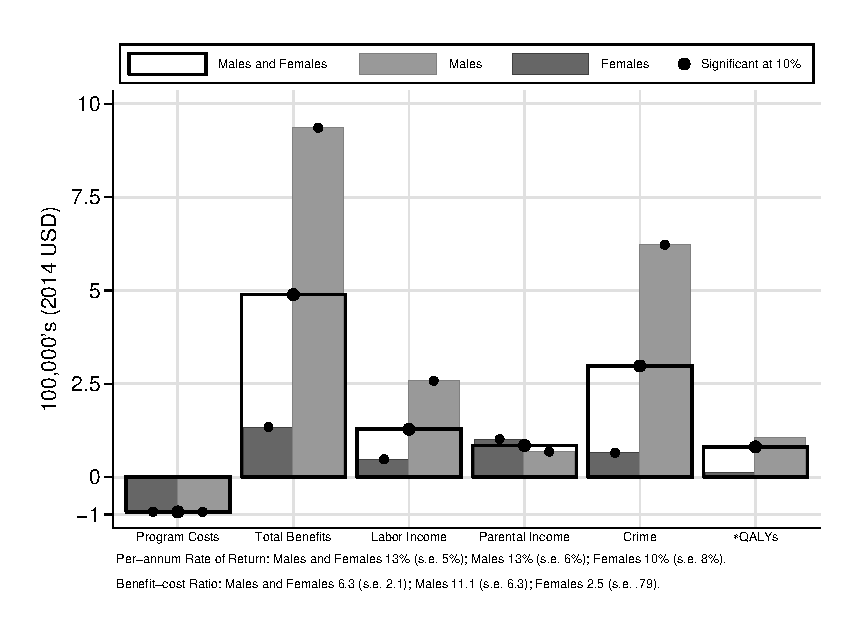
\includegraphics[width=.7\columnwidth]{output/abccare_npvssumm.eps}
\floatfoot{
\footnotesize
Note: This figure displays the life-cycle net present values of the main components of the cost/benefit analysis of ABC/CARE from birth to age 79, discounted to birth at a rate of 3\%.  By ``net" we mean that each component represents the total value for the treatment group minus the total value for the control group. Program costs: the total cost of implementing ABC/CARE. Total net benefits: the total net benefits of \textit{all} the components we consider. Labor income: total individual labor income from ages 20 to the retirement of program participants (assumed to be age 67). Parental income: total parental labor income of the parents pf the participants from when the participants were ages 1.5 to 21. Crime: the total cost of crime (judicial and victimization costs). For display simplicity, the following components are omitted from the figure: (i) cost of alternative preschool paid by the control group children parents; (ii) transfer income from the government; (iii) disability benefits and social security claims; (iv) costs of increased individual and maternal education; (v) total medical public and private costs. Inference is based on non-parametric, one-sided $p$-values from the empirical bootstrap distribution. We highlight point estimates significant at the $10\%$ level.\\
*Labor Income results by gender indicate a statistically significant net present value of $\$308,825$ (2014 USD) for males; this value is $\$50,580$ (2014 USD) for females and it is not statistically significant.\\
**QALYs refers to the quality-adjusted life years. Any gain corresponds to better health conditions through age 79.\\}
\end{sidewaysfigure}

The rest of the paper justifies and interprets these estimates. We proceed in the following way. Section~\ref{section:background} discusses main features of ABC/CARE. Section~\ref{section:methodsquestions} defines the parameters of interest. Section~\ref{section:methodology} discusses our approaches to inference for vectors of treatment effects. We report step-down $p$-values for each vector. We summarize standard treatment effects for ABC/CARE. We account for multiple hypothesis testing by adjusting $p$-values for the multiplicity of reported outcomes to avoid cherry-picking ``significant'' results.\footnote{\citet{Lehman_Romano_2005_AnnStat,Romano_Shaikh_2006_AnnStat}. For an application, see, e.g., \cite{Heckman_Moon_etal_2010_QE}.} We also use combining functions that summarize the \emph{number} of beneficial outcomes, as well as the number of statistically significant beneficial outcomes. Section~\ref{section:c-functions} presents inference for combining functions.

Our main approach for summarizing the multiple program treatment effects uses benefit/cost and rate of return analyses. These parameters provide economically interpretable summaries of the program and its components. Section~\ref{section:cbamethodology} discusses our approaches to predicting life-cycle outcomes to conduct the benefit/cost analyses and evidence supporting the assumptions underlying it. Section~\ref{section:cbaresults} presents and analyzes estimates of benefit/cost ratios and rates of return.

Section~\ref{section:conclusion} summarizes the paper. There are substantial benefits that differ by gender. In terms of treatment effects, females benefit across more domains. However, the monetized value of the treatment effects is substantially greater for males. This discrepancy is largely driven by labor income and health benefits, as well as reduced crime for males. Males seem to be more sensitive than females to being taken away from their mothers and placed in lower quality alternative early childcare programs.

\section[Background and Data Sources]{Background and Data Sources} \label{section:background}

\subsection{Overview}

ABC/CARE targeted disadvantaged children in Chapel Hill/Durham, North Carolina.\footnote{Both ABC and CARE were designed and implemented by researchers at the Frank Porter Graham Center of the University of North Carolina in Chapel Hill.} Table~\ref{tab:programcomparison} presents an overview and compares the two virtually congruent programs. Appendix~\ref{appendix:background} describes these programs in detail. Here, we summarize their main features.

The goals of these programs were to enhance the early-life skills of a disadvantaged population. The program supported language, motor, and cognitive development and developed socio-emotional competencies considered crucial for school success including task-orientation, ability to communicate, independence, and pro-social behavior.\footnote{\citet{Ramey_Collier_etal_1976_CarolinaAbecedarianProject, Ramey_etal_1985_Project-CARE_TiECSE, Sparling_1974_Synth_Edu_Infant_SPEECH, Wasik_Ramey_etal_1990_CD, Ramey-etal_2012-ABC}.}

The program provided individualized treatment. Each child's progress was recorded and learning activities were appropriately adjusted every 2 to 3 weeks. Environments were organized to promote pre-literacy and access to a rich set of learning tools.\footnote{The ``LearningGames'' approach was implemented by infant and toddler caregivers in 1:1 child-adult interactions. Each ``LearningGames'' activity state a developmentally-appropriate objective, the necessary materials, directions for teacher behavior, and expected child outcome.} The curriculum emphasized active learning experiences, dramatic play, and basic ideas of order and category (``pre-academic skills''), as well as discipline and the ability to interact with and respect others.  At later ages (3 through 5), the program became increasingly structured, focusing on the development of ``socio-linguistic and communicative competence.''\footnote{\citet{Ramey-et-al_1977_Intro-to-ABC, Haskins_1985_CD, Ramey_1981_Modification, Ramey_Campbell_1979_SR, Ramey_Smith_1977_AJMD, Ramey_McGinness_etal_1982_Abecedarianapproach, Sparling_Lewis_1979_BOOKLearninggamesFirstThree,Sparling_Lewis_1984_BOOKLearningGamesThreesFours}.}

ABC recruited four cohorts of predominately African American children born between 1972 and 1976. CARE recruited two cohorts of children, born between 1978 and 1980. The recruitment processes for each study were identical. Potential participant families were referred to researchers by local social service agencies and hospitals at the beginning of the mother's last trimester of pregnancy. Eligibility was determined by a score of 11 or above on a High-risk Index (HRI).\footnote{See Appendix~\ref{appendix:background} for details on the construction of the HRI. Maternal education, parental IQ, presence of the father, family income, and father's job stability are its major components.}

As shown in Table~\ref{tab:programcomparison}, the design and implementation of both ABC and CARE were very similar. ABC had two phases, the first of which lasted from birth until age 5. In this phase, children were randomly assigned to either a treatment group that received center-based childcare or a control group. The second phase of treatment consisted of child academic support through home visits from ages 5 through 8. CARE consisted of two treatment phases as well. They were very similar to those of ABC. The first phase of CARE, also lasting from birth until age 5, contained an additional treatment arm, home visits, designed to study the effects of improving home environments on child development.\footnote{\citet{Wasik_Ramey_etal_1990_CD}.} The second phase was only randomized in ABC.

Our analysis focuses on the first phase and pools the treatment group in CARE that received the center-based ABC curriculum with the ABC treatment group. We do not use the data on the CARE treatment group that only received family education.\footnote{\citet{Campbell_Conti_etal_2014_EarlyChildhoodInvestments} and \citet{ABCCARE_Dataset} show that there is no effect of the CARE family education component alone.} We analyze the first stage of both programs (through age 5).\footnote{The second-phase treatment of ABC/CARE had very weak, if any, effects (for evidence, see \citealp{Campbell_Conti_etal_2014_EarlyChildhoodInvestments} and \citealp{ABCCARE_Dataset}). \citet{Campbell_Conti_etal_2014_EarlyChildhoodInvestments} establish the validity of pooling the data across the second arms of the experiments.}

\begin{table}[!htbp]
\centering
\caption{ABC and CARE, Program Comparison} \label{tab:programcomparison}
\begin{adjustbox}{max width=\textwidth}
\begin{threeparttable}
	\small
	\begin{table}[H]
\begin{center}
\begin{threeparttable}
\caption{ABC and CARE, Programs Comparison} \label{tab:programcomparison}
\scriptsize
\scalebox{.9}{\begin{tabular}{L{4cm} L{7cm} L{5cm}}
\hline \hline
& \multicolumn{1}{c}{ABC}& \multicolumn{1}{c}{CARE}\\
\hline 
Program Overview &&\\
\hspace{.5cm} Years Implemented &1972--1982&1978--1985\\
\hspace{.5cm} Age of Entry/Exit & birth to 5 years old &\checkmark\\
\hspace{.5cm} Initial Sample &122&64\\
\hspace{.5cm} \# of Cohorts &4&2\\
\midrule
Eligibility & socio-economic disadvantage according to a multi-factor index (see Section \ref{section:eligibility})&\checkmark\\
 \midrule
Control &&\\
\hspace{.5cm} N &54&23\\
\hspace{.5cm} Compensation & Diapers from birth to age 3, unlimited formula from birth to 15 months & \checkmark \\
\hspace{.5cm} Treatment Substitution & 70\% & $\sim$ 70\%\\
\midrule
Treatment & Center-based childcare & Center-based childcare and family education\\
\hspace{.5cm} \textbf{Center-base} &&\\
\hspace{.5cm} \textbf{Childcare} &&\\
\hspace{.5cm} N &57&17\\
\hspace{.5cm} Intensity &6.5--9.75 hours a day for 50 weeks per year&\checkmark\\
\hspace{.5cm} Components & Instruction, medical care, nutrition, social services &\checkmark\\
\hspace{.5cm} Staff-to-child Ratio &1:3 during ages 0--1 &\checkmark\\
&1:4--5 during age 1--4 &\checkmark\\&1:5--6 during ages 4--5 &\checkmark\\
\hspace{.5cm} Staff Qualifications &Mixed diplomas; experienced&\checkmark\\
\hspace{.5cm} \textbf{Family Education} & Not part of the program &24\\
\hspace{.5cm} Intensity && One hour-long home visits. 2--3 per month during ages 0--3. 1--2 per month during ages 4--5\\
\hspace{.5cm} Curriculum & & Social and mental stimulation; parent-child interaction\\
\hspace{.5cm} Staff-to-child Ratio &&1:1\\
\hspace{.5cm} Staff Qualifications &&Home visitor training\\
\midrule
 School-age Treatment \\
 \hspace{.5cm} N&46&39\\
\hspace{.5cm} Intensity &Every other week& \checkmark\\
\hspace{.5cm} Components &Parent-teacher meetings& \checkmark\\
\hspace{.5cm} Curriculum & Reading and math &\checkmark\\
\hspace{.5cm} Staff-to-child Ratio &1:1&\checkmark\\
\hspace{.5cm} Staff Qualifications &Graduate degree and training in special education & \checkmark\\
\midrule
Data Availability \\
Questionnaires & Ages 0--5, 8, 12, 15, 21, 30--34 & Ages 0--5, 8, 12, 21, 30--34 \\
Parent Interview & Ages 0--5, 8, 12, 15, 21& Ages 0--5, 9, 12 \\  
Health Follow-up & Ages 30--34&\checkmark\\
\hline \hline
\end{tabular}}
\footnotesize
\begin{tablenotes}
\item Note: This table compares the main elements of ABC and CARE, summarized within this section.
\end{tablenotes}
\end{threeparttable}
\end{center}
\end{table}
\begin{tablenotes}
\small
\item Note: This table compares the main elements of ABC and CARE, summarized in this section. A \checkmark\ indicates that ABC and CARE had the same characteristic. A blank space indicates that the specific component was not part of the program.
\end{tablenotes}
\end{threeparttable}
\end{adjustbox}
\end{table}

For both programs, from birth until the age of 8, data were collected annually on cognitive and socio-emotional skills, home environments, family structure, and family economic characteristics. After age 8, data on cognitive and socio-emotional skills, education, and family economic characteristics were collected at ages 12, 15, 21, and 30.\footnote{At age 30, measures of cognitive skills are unavailable for both ABC and CARE.} In addition, we have access to unique administrative criminal records and a full medical survey at age 34. This allows us to study the long-term effects of the programs along multiple dimensions of human development.\footnote{See Appendix~\ref{appendix:data} for a more comprehensive description of the data. In Appendix~\ref{appendix:randomization}, we document the balance in observed baseline characteristics across the treatment and control groups, once we drop the individuals for whom we have crime or health information, for which there is substantial attrition. Further, the methodology we propose addresses missing information in either of these two outcome categories.}

\subsection{Randomization Protocol and Compromises} \label{section:randomization}

Randomization for ABC/CARE was conducted at the family level. Pairs of siblings and twins were jointly randomized into either treatment or control groups.\footnote{Sibling pairs occurred when the two siblings were close enough in age such that both of them were eligible for the program.} Although we know that pairing was based on the HRI, maternal education, maternal age, and gender of the subject, we do not know the original pairs. ABC collected an initial sample of 122 subjects. 22 subjects did not complete the first-phase of treatment as initially assigned by the randomization. We characterize each of the cases in Appendix~\ref{appendix:background} and document that our estimates are robust when we adjust for missing data using standard methods. We conduct a comparable analysis for the CARE sample.

\subsection{Control Group Substitution}

In ABC/CARE, many control group members attended alternative preschools.\footnote{See \cite{Heckman_Hohmann_etal_2000_QJE} on the issue of substitution bias in social experiments.} In ABC, \treatsubsabc\ of controls were enrolled in one of 11 local center-based childcare centers. In CARE, \treatsubscarec\ of the controls were enrolled in alternative preschools. Figure~\ref{fig:salmonella} shows the enrollment of the control families into alternative preschools by age of child for the full sample, and for those who enrolled in any alternative preschool, however long. Enrollment increases with the age of children.

Figure~\ref{fig:treatsubcare_2} shows the proportion of the sample enrolled in an alternative school at a given age who persist in alternative care at the next age. Once enrolled, they stay enrolled, and children generally go for a full year.  Figure~\ref{fig:treatsubcare} shows (for each program) the cumulative distribution of the proportion of the first five years that control subjects were enrolled in alternative preschools. Figure~\ref{fig:proportion-alt-pre} shows the distribution of time spent in the alternative program for all control group participants.

Although not statistically significant in many cases, children in the control group who attend alternative preschools are less economically disadvantaged at baseline when compared to children who stay at home. Disadvantage is measured by: maternal education, maternal IQ, Apgar scores at minutes 1 and 5, and the high-risk index defining ABC/CARE eligibility. Children who attend alternative preschools have fewer siblings. On average, they are children of mothers who are more likely to be working at baseline.\footnote{Statistically significant at 10\%.} \emph{It is the mothers of female children who are much more likely to use alternative preschools if assigned to the control group.} See Table~\ref{table:controlsubscharacteristics} in Appendix~\ref{appendix:background} for tests of differences between these variables across children in the control group who attend and who do not attend alternative preschools. There are no differences in use of alternative preschools by gender.

Most of the alternative preschools received federal subsidies and were subject to the federal regulations of the era.\footnote{Appendix~\ref{appendix:tetanus} discusses the federal standards of that day. See \citet{Department-of-Health_1968_DayCareRequirements,NCGA_1971_House-Bill-100,Ramey-et-al_1977_Intro-to-ABC,Ramey_Campbell_1979_SR,Ramey_McGinness_etal_1982_Abecedarianapproach, Burchinal_Campbell_etal_1997_CD}.} The access of control-group children to alternative programs affects the interpretation of estimated treatment effects. We discuss this issue next.

\begin{sidewaysfigure}[!htbp]
\centering
\caption{Control Substitution Characteristics, ABC/CARE Control Group}\label{fig:control-sub}
\begin{subfigure}[h]{0.4\textwidth}
	\centering
	\caption{Enrollment by Age} \label{fig:salmonella}
		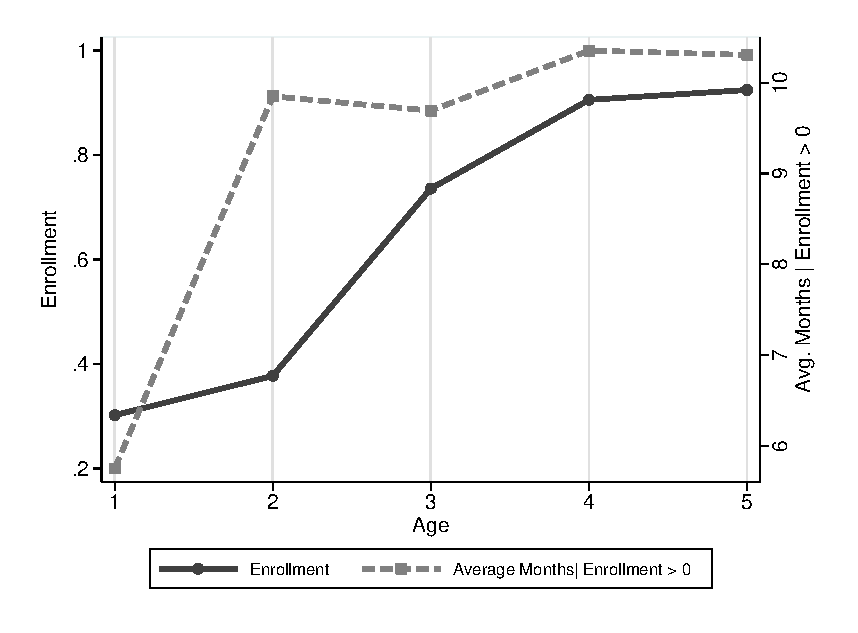
\includegraphics[width=\textwidth]{output/abccare_Valtenrollment.eps}
\end{subfigure}
\begin{subfigure}[h]{0.4\textwidth}
		\centering
		\caption{Enrollment Dynamics} \label{fig:treatsubcare_2}
		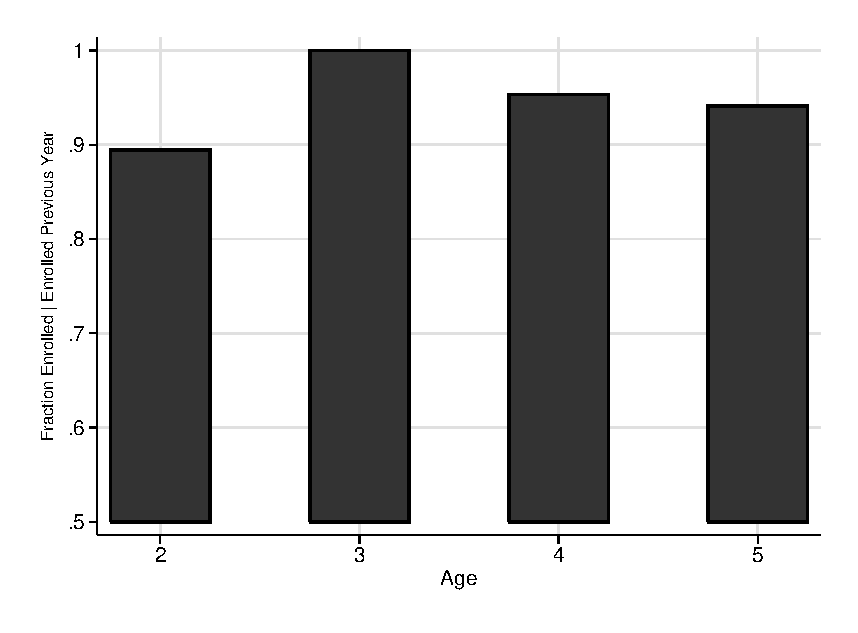
\includegraphics[width=\textwidth]{output/abccare_Vprobs.eps}
\end{subfigure}\\
\begin{subfigure}[h]{0.4\textwidth}
		\centering
		\caption{Cumulative Enrollment} \label{fig:treatsubcare}
		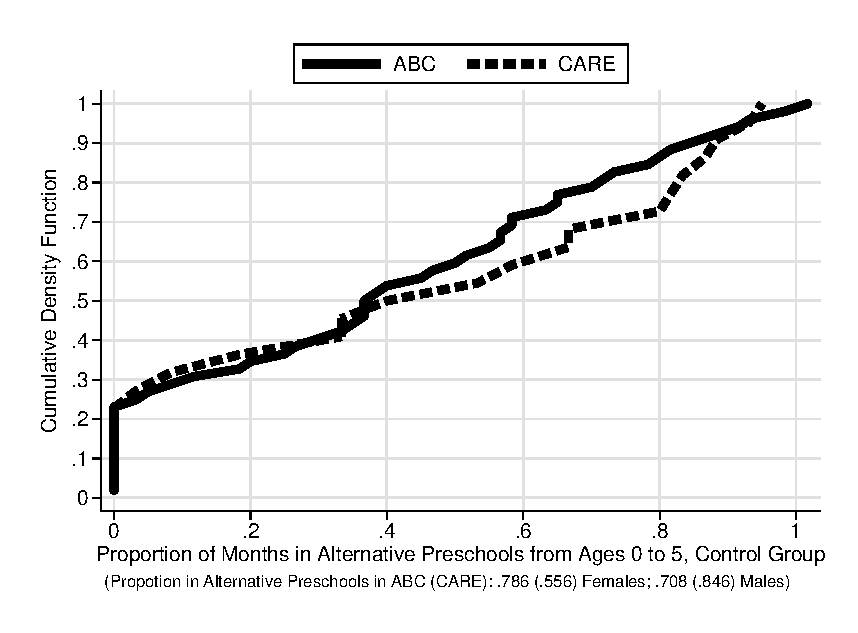
\includegraphics[width=\textwidth]{output/abccare_controlcontamination.eps}
\end{subfigure}
\begin{subfigure}[h]{0.4\textwidth}
	\centering
	\caption{Enrollment Intensity} \label{fig:proportion-alt-pre}
		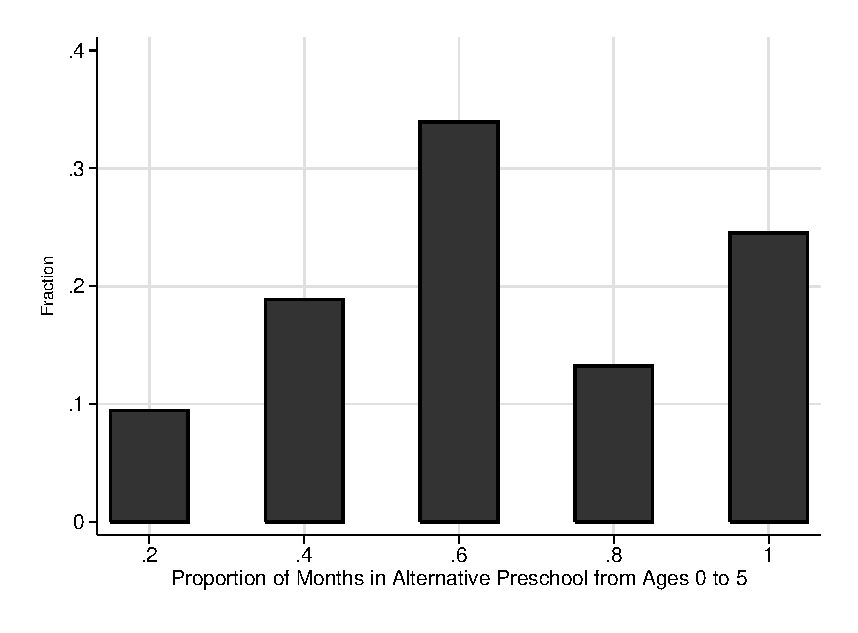
\includegraphics[width=\textwidth]{output/abccare_Vfractimes.eps}
\end{subfigure}%

\footnotesize \justify
Note: Panel (a) displays the fraction enrolled in alternative preschools of ABC/CARE control group by age in the left axis and average number of months in alternative preschool by age in the right axis. Both plots in Panel (a) are conditional on enrollment. Panel (b) displays the fraction of ABC/CARE control-group children enrolled in preschool, conditional on being enrolled in the previous age (at least one month). Panel (c) displays the cumulative distribution function of enrollment in alternative preschools of the ABC/CARE control group. Panel (d) displays the fraction of children in the ABC/CARE control group enrolled in alternative preschools (fraction of children who were enrolled in alternative preschools 20\%, 40\%, 60\%, 80\%, and 100\% of the time, from ages 0 to 5). \\
\end{sidewaysfigure}

\section{Notation and Parameters of Interest} \label{section:methodsquestions}

Random assignment to treatment does not guarantee that conventional treatment effects answer policy-relevant questions. In this paper, we define and estimate three parameters that address different policy questions.

We assume that life cycles consist of $T+1$ discrete periods. The treatment phase is the first $\bar{t}$ periods of life $\left[0,\dots,\bar{t}\right]$. We have data up through age $t^{*}>\bar{t}$. We lack follow-up data on the remainder of life $(t^*,\dots,T]$. $W=1$ indicate that parents wish to participate in the program.\footnote{Individual subscripts are omitted to improve clarity.} $R \in \{0,1\}$ where $R=1$ indicates that a child is randomized into eligibility to participate in the program. Let $D$ indicate participation in the program.

Individuals are eligible to participate in the program if baseline background variables $\bm{B}\in\mathcal{B}_0$. In this paper, $\mathcal{B}_0$ is the set of scores on the high risk index (HRI) previously discussed.

As it turns out, in the ABC/CARE study, the eligible persons ($\bm{B}\in\mathcal{B}_0$) given the option to participate choose to do so $(W=1\text{, and } D=R)$ generally.\footnote{There are minimal cases of non-compliance and attrition. See Appendix~\ref{appendix:background} for details and Appendix~\ref{appendix:assessingcc} for evidence indicating that these cases minimally bias our results.} Thus, we can safely interpret the treatment effects generated by the experiment as average treatment effects for the population for which $\bm{B}\in\mathcal{B}_0$ and not just treatment effects for the treated (\textbf{TOT}). There are few dropouts from the program. \emph{Ex ante}, parents perceived that ABC/CARE was superior to other childcare alternatives.

Let $\bm{Y}^1_t$ be the outcome vector for the treated. $\bm{Y}^0_t$ is the outcome vector for those denied treatment in the program. In principle, life-cycle treatment effects for the controls can depend on the exposures to treatment or to the various alternatives at each age. It would be desirable to estimate treatment effects for each possible exposure but our samples are too small to make credible estimates for such detailed exposures.

We simplify the analysis by creating two categories of control status. ``$H$'' indicates that the child is in home care throughout the entire length of the program. ``$C$'' indicates that the child was in an alternative preschool for any amount of time. We test different categorizations in our empirical analysis reported below.

We thus compress a complex reality into two counterfactual outcome states at age $t$ for control group members:
\begin{align*}
\bm{Y}_{t,H}^0 \quad &: \quad \textbf{ Subject received home care exclusively} \\
\bm{Y}_{t,C}^0 \quad &: \quad \textbf{ Subject received some alternative childcare}.
\end{align*}

We define $V$ as a dummy variable indicating participation by control-group children in an alternative preschool. $V=0$ denotes staying at home. The outcome when a child is in control status is $\bm{Y}^0_t$:
\begin{equation}
\bm{Y}^0_t : = \left( 1 - V \right) \bm{Y}^0_{t,H} + \left( V \right) \bm{Y}^0_{t,C}.
\end{equation}

One parameter of interest addresses the question: what is the effect of the program as implemented? This is the effect of the program compared to the next best alternative as perceived by the parents and is defined by
\begin{equation}\label{eq:effect}
\bm{\Delta}_t := \mathbb{E} \left[ \bm{Y}^1_t -  \bm{Y}^0_t | W =1 \right] = \mathbb{E} \left[\bm{Y}^1_t - \bm{Y}^0_t | \bm{B} \in \mathcal{B}_0 \right],
\end{equation}
where the second equality follows because everyone eligible wants to participate in the program. For the sample of eligible persons, this parameter addresses the effectiveness of the program relative to the quality of all alternatives available when the program was implemented.

It is also fruitful to ask: what is the effectiveness of the program with respect to a counterfactual world in which the child stays at home full time? The associated causal parameter for those who would choose to keep the child at home is:
\begin{equation}\label{eq:influenza}
\bm{\Delta}_t \left(V = 0 \right) : =   \mathbb{E} \left[ \bm{Y}^1_t - \bm{Y}^0_t | V = 0, W = 1 \right] := \mathbb{E} \left[\bm{Y}^1_{t} - \bm{Y}^0_{t,H} | V = 0, \bm{B} \in \mathcal{B}_0 \right].
\end{equation}
It is also useful to assess the average effectiveness of a program relative to attendance in an alternative preschool for those who would choose an alternative is:
\begin{equation}\label{eq:smallpox}
\bm{\Delta}_t \left( V =1 \right) : =   \mathbb{E} \left[ \bm{Y}^1_t - \bm{Y}^0_t | V = 1, W = 1 \right] := \mathbb{E} \left[\bm{Y}^1_t - \bm{Y}^0_{t,C} | V = 1, \bm{B} \in \mathcal{B}_0 \right].
\end{equation}
Random assignment to treatment does not directly identify \eqref{eq:influenza} or \eqref{eq:smallpox}. Econometric methods are required to identify these parameters. We characterize the determinants of choices and our strategy for controlling for selection into \ref{appendix:results} and \ref{appendix:methodology} below.

\section{Summarizing Multiple Treatment Effects} \label{section:methodology}

ABC/CARE has rich longitudinal data on multiple outcomes over multiple periods of the life cycle. Summarizing these effects in an interpretable way is challenging.\footnote{Appendix~\ref{appendix:results} presents step-down $p$-values for the blocks of outcomes that are used in our benefit/cost analysis which we summarize in this section (\citealp{Lehman_Romano_2005_AnnStat} and \citealp{Romano_Shaikh_2006_AnnStat}).} Simpler, more digestible summary measures are useful for understanding the main empirical regularities in our data. This section discusses our approach to summarizing vectors of treatment effects using combining functions that count the proportion of treatment effects by category that show beneficial outcomes.

Consider a block of $N_l$ outcomes indexed by set $Q_l = \{1,\dots,N_l\}$. Let $j \in Q_l$ be a particular outcome within block $l$. Associated with it is a mean treatment effect
\begin{equation}
\Delta_{j,t} : = \mathbb{E} \left[ Y^1_{j,t} - Y^0_{j,t} | \bm{B} \in \mathcal{B}_0 \right].
\end{equation}

We assume that outcomes can be ordered so that $\Delta_{j,t} >0$ is beneficial.\footnote{All but 5\% of the outcomes we study can be ranked in this fashion. See Appendix~\ref{appendix:results} for our classification.} We summarize the estimated effects of the program on outcomes within the block by the number of positive counts within block $l$:
\begin{equation}
C_l = \sum^{N_l}_{j=1} 1 (\hat{\Delta}_{j,t} >0).
\end{equation}
The proportion of beneficial outcomes in block $l$ is $C_l / N_l$.\footnote{In our empirical application we consider all the outcomes as a block, and then different blocks grouped according to common categories---e.g., skills, health, crime.}

Let $\mathcal{L}$ be the set of blocks. Under the null hypothesis of no treatment effects for all $j \in Q_l, l \in \mathcal{L}$, and assuming the validity of asymptotic approximations, $C_l / N_l$ should be centered around $1/2$. We bootstrap to obtain $p$-values for the null for each block and over all blocks. We also count the individually beneficial treatment effects that are statistically significant in the sets of outcomes across each of the groups indexed by the set $Q_l$. Using a 10\% significance level, on average 10\% of all outcomes should be ``significant'' at the 10\% level even if there is no treatment effect of the program. We provide evidence against both null hypotheses.\footnote{We present $p$-values for these hypotheses and a number of combining functions by outcome categories in Appendix~\ref{appendix:results}.}

Combining counts across all blocks enables us to avoid (i) arbitrarily picking outcomes that have statistically significant effects---``cherry picking''; or (ii) arbitrarily selecting blocks of outcomes to correct the $p$-values when accounting for multiple hypothesis testing.

\section{Empirical Estimates of Treatment Effects and Combining Functions}\label{section:c-functions}

ABC/CARE has hundreds of treatment effects corresponding to all of the measures collected in the multiple waves of the longitudinal surveys.\footnote{For estimates of treatment effects for each outcome analyzed, see Appendix~\ref{appendix:results}.} Reporting these treatment effects in the text would overwhelm the reader. Here we report estimates of the main treatment effects that underlie our benefit/cost and rate of return analyses.\footnote{Appendix~\ref{appendix:results} reports treatment effects and step-down $p$-values for all the outcomes analyzed. These account for multiple hypothesis testing as in \citet{Lehman_Romano_2005_AnnStat,Romano_Shaikh_2006_AnnStat}.}

Evidence from ABC/CARE and other early childhood programs is often criticized because of their small sample sizes.\footnote{See, e.g., \cite{Murray_2013_GivingKids_JJHBOOK}.} An extensive analysis reported in \citet{Campbell_Conti_etal_2014_EarlyChildhoodInvestments} shows that asymptotic inference and small sample permutation-based inference closely agree when applied to ABC/CARE data. For this reason, we use large sample inference throughout this paper.\footnote{Unless otherwise specified, the inference we present throughout the paper is based on $1,000$ draws from the empirical bootstrap distribution. $p$-values are one-sided, non-parametric. We highlight values when estimates are significant at $10\%$. For estimations using combining different datasets, we bootstrap all datasets and combine them to form bootstrap draws. Inference based on permutation tests is available on request.} We adjust all estimates for sample attrition using Horvitz--Thompson \citeyearpar{Horvitz_Thompson_1952_JASA} inverse probability estimators (see Appendix~\ref{appendix:attrition} for details).

We account for control group substitution using a variety of econometric procedures: (a) matching, (b) instrumental variables, and (c) control functions (selection estimators). We rely on matching to generate the main inferences in this paper because the available instruments and exclusion restrictions are weak.\footnote{We present estimates based on kernel matching. A full set of results based on propensity score matching generates similar results and is available under request.} Estimates from all of these procedures are in rough agreement, although the standard errors associated with IV and control function estimators are large. For further discussion, see Appendix~\ref{appendix:amethodology}.

\subsection{Estimated Treatment Effects}

The results for females show that the program increases the employment and incomes of participants as adults, their high school graduation, college graduation, and parental income. It reduces participant arrests (see Table~\ref{table:tescombined}). These results strengthen when we compare treatment with the alternative of staying exclusively at home.

The results for males are different. Treated subjects reported lower drug use and blood pressure. There are also effects on labor income and education. The results for employment, hypertension, blood pressure, and graduation from a 4-year college are strengthened when comparing the treatment group to those subjects who attend alternative preschools.

\newgeometry{top=.6in, bottom=.8in, left=.8in, right=.8in}
\begin{table}[!htbp]
\centering
\begin{threeparttable}
\caption{Treatment Effects on Selected Outcomes}\label{table:tescombined}
\begin{scriptsize}
  \begin{tabular}{ccccccccccc}
  \toprule
   Category & Variable & Age & (1) & (2) & (3) & (4) & (5) & (6)\\

    \midrule
     \multicolumn{9}{c}{\textbf{\emph{Females}}} \\ \\
    %cat 3
  \mc{1}{l}{\scriptsize{Parental Income}} &  \mc{1}{l}{\scriptsize{Parental Labor Income}} & \mc{1}{c}{\scriptsize{3.5}} & \mc{1}{c}{\scriptsize{2,756}} & \mc{1}{c}{\scriptsize{3,277}} & \mc{1}{c}{\scriptsize{10,509}} & \mc{1}{c}{\scriptsize{8,601}} & \mc{1}{c}{\scriptsize{-2,519}}  & \mc{1}{c}{\scriptsize{3,762}} \\  

  &   &  & \mc{1}{c}{\scriptsize{(0.206)}} & \mc{1}{c}{\scriptsize{(0.181)}} & \mc{1}{c}{\scriptsize{\textbf{(0.051)}}} & \mc{1}{c}{\scriptsize{\textbf{(0.058)}}} & \mc{1}{c}{\scriptsize{(0.614)}} & \mc{1}{c}{\scriptsize{(0.182)}} \\  

   &  & \mc{1}{c}{\scriptsize{12}} & \mc{1}{c}{\scriptsize{13,633}} & \mc{1}{c}{\scriptsize{19,386}} & \mc{1}{c}{\scriptsize{33,624}} & \mc{1}{c}{\scriptsize{26,474}} & \mc{1}{c}{\scriptsize{11,176}} & \mc{1}{c}{\scriptsize{18,629}} \\  

  &   &  & \mc{1}{c}{\scriptsize{\textbf{(0.061)}}} & \mc{1}{c}{\scriptsize{\textbf{(0.036)}}} & \mc{1}{c}{\scriptsize{(0.133)}} & \mc{1}{c}{\scriptsize{\textbf{(0.010)}}} & \mc{1}{c}{\scriptsize{(0.138)}} & \mc{1}{c}{\scriptsize{\textbf{(0.015)}}} \\  

 &    & \mc{1}{c}{\scriptsize{15}} & \mc{1}{c}{\scriptsize{8,565}} & \mc{1}{c}{\scriptsize{9,322}} & \mc{1}{c}{\scriptsize{5,533}} & \mc{1}{c}{\scriptsize{8,435}} & \mc{1}{c}{\scriptsize{8,817}} & \mc{1}{c}{\scriptsize{10,480}} \\  

  &   &  & \mc{1}{c}{\scriptsize{\textbf{(0.052)}}} & \mc{1}{c}{\scriptsize{\textbf{(0.090)}}} & \mc{1}{c}{\scriptsize{(0.354)}} & \mc{1}{c}{\scriptsize{(0.361)}} & \mc{1}{c}{\scriptsize{(0.114)}} & \mc{1}{c}{\scriptsize{\textbf{(0.058)}}} \\  

  &   & \mc{1}{c}{\scriptsize{21}} & \mc{1}{c}{\scriptsize{5,708}} & \mc{1}{c}{\scriptsize{6,944}} & \mc{1}{c}{\scriptsize{41,245}} & \mc{1}{c}{\scriptsize{25,135}} & \mc{1}{c}{\scriptsize{4,608}} & \mc{1}{c}{\scriptsize{3,926}} \\  

  &   &  & \mc{1}{c}{\scriptsize{(0.130)}} & \mc{1}{c}{\scriptsize{(0.214)}} & \mc{1}{c}{\scriptsize{\textbf{(0.023)}}} & \mc{1}{c}{\scriptsize{\textbf{(0.001)}}} & \mc{1}{c}{\scriptsize{(0.255)}} & \mc{1}{c}{\scriptsize{(0.265)}} \\  

 \mc{1}{l}{\scriptsize{Education}} &   \mc{1}{l}{\scriptsize{Graduated High School}} & \mc{1}{c}{\scriptsize{30}} & \mc{1}{c}{\scriptsize{0.253}} & \mc{1}{c}{\scriptsize{0.110}} & \mc{1}{c}{\scriptsize{0.561}} & \mc{1}{c}{\scriptsize{0.596}} & \mc{1}{c}{\scriptsize{-0.027}} & \mc{1}{c}{\scriptsize{0.066}} \\  

  &   &  & \mc{1}{c}{\scriptsize{\textbf{(0.012)}}} & \mc{1}{c}{\scriptsize{(0.208)}} & \mc{1}{c}{\scriptsize{\textbf{(0.001)}}} & \mc{1}{c}{\scriptsize{\textbf{(0.000)}}} & \mc{1}{c}{\scriptsize{(0.431)}} & \mc{1}{c}{\scriptsize{(0.310)}} \\  

  &  \mc{1}{l}{\scriptsize{Graduated 4-year College}} & \mc{1}{c}{\scriptsize{30}} & \mc{1}{c}{\scriptsize{0.134}} &  \mc{1}{c}{\scriptsize{0.119}}  & \mc{1}{c}{\scriptsize{0.112}} & \mc{1}{c}{\scriptsize{0.219}} & \mc{1}{c}{\scriptsize{0.095}} & \mc{1}{c}{\scriptsize{0.094}} \\  

  &   &  & \mc{1}{c}{\scriptsize{\textbf{(0.078)}}} &  \mc{1}{c}{\scriptsize{\textbf{(0.099)}}} & \mc{1}{c}{\scriptsize{(0.140)}} & \mc{1}{c}{\scriptsize{\textbf{(0.012)}}} & \mc{1}{c}{\scriptsize{(0.242)}} & \mc{1}{c}{\scriptsize{(0.210)}} \\  

  &  \mc{1}{l}{\scriptsize{Years of Education}} & \mc{1}{c}{\scriptsize{30}} & \mc{1}{c}{\scriptsize{2.143}} & \mc{1}{c}{\scriptsize{1.715}} & \mc{1}{c}{\scriptsize{3.370}} & \mc{1}{c}{\scriptsize{3.925}} & \mc{1}{c}{\scriptsize{1.238}} & \mc{1}{c}{\scriptsize{1.412}} \\  

  &   &  & \mc{1}{c}{\scriptsize{\textbf{(0.000)}}} & \mc{1}{c}{\scriptsize{\textbf{(0.007)}}} & \mc{1}{c}{\scriptsize{\textbf{(0.001)}}} & \mc{1}{c}{\scriptsize{\textbf{(0.000)}}} & \mc{1}{c}{\scriptsize{\textbf{(0.055)}}} & \mc{1}{c}{\scriptsize{\textbf{(0.023)}}} \\  

  \mc{1}{l}{\scriptsize{Labor Income}} &  \mc{1}{l}{\scriptsize{Employed}} & \mc{1}{c}{\scriptsize{30}} & \mc{1}{c}{\scriptsize{0.131}} & \mc{1}{c}{\scriptsize{0.079}} & \mc{1}{c}{\scriptsize{0.395}} & \mc{1}{c}{\scriptsize{0.340}} & \mc{1}{c}{\scriptsize{-0.004}} & \mc{1}{c}{\scriptsize{0.070}} \\  

 &    &  & \mc{1}{c}{\scriptsize{\textbf{(0.084)}}} & \mc{1}{c}{\scriptsize{(0.222)}} & \mc{1}{c}{\scriptsize{\textbf{(0.001)}}} & \mc{1}{c}{\scriptsize{\textbf{(0.037)}}} & \mc{1}{c}{\scriptsize{(0.483)}} & \mc{1}{c}{\scriptsize{(0.249)}} \\  

 &   \mc{1}{l}{\scriptsize{Labor Income}} & \mc{1}{c}{\scriptsize{30}} & \mc{1}{c}{\scriptsize{2,548}} & \mc{1}{c}{\scriptsize{2,412}} & \mc{1}{c}{\scriptsize{10,256}} & \mc{1}{c}{\scriptsize{14,862}} & \mc{1}{c}{\scriptsize{-1,078}} & \mc{1}{c}{\scriptsize{-822}} \\  

 &    &  & \mc{1}{c}{\scriptsize{(0.337)}} & \mc{1}{c}{\scriptsize{(0.363)}} & \mc{1}{c}{\scriptsize{(0.154)}} & \mc{1}{c}{\scriptsize{\textbf{(0.020)}}} & \mc{1}{c}{\scriptsize{(0.413)}} & \mc{1}{c}{\scriptsize{(0.457)}} \\  

  \mc{1}{l}{\scriptsize{Crime}} &  \mc{1}{l}{\scriptsize{Total Felony Arrests}} & \mc{1}{c}{\scriptsize{Mid-30s}} & \mc{1}{c}{\scriptsize{-0.328}} & \mc{1}{c}{\scriptsize{-0.394}} & \mc{1}{c}{\scriptsize{-1.006}} & \mc{1}{c}{\scriptsize{-0.965}} & \mc{1}{c}{\scriptsize{-0.083}} & \mc{1}{c}{\scriptsize{0.005}} \\  

   &  &  & \mc{1}{c}{\scriptsize{\textbf{(0.085)}}} & \mc{1}{c}{\scriptsize{\textbf{(0.078)}}} & \mc{1}{c}{\scriptsize{(0.119)}} & \mc{1}{c}{\scriptsize{\textbf{(0.096)}}} & \mc{1}{c}{\scriptsize{(0.237)}} & \mc{1}{c}{\scriptsize{(0.469)}} \\  

   & \mc{1}{l}{\scriptsize{Total Misdemeanor Arrests}} & \mc{1}{c}{\scriptsize{Mid-30s}} & \mc{1}{c}{\scriptsize{-0.973}} & \mc{1}{c}{\scriptsize{-1.212}} & \mc{1}{c}{\scriptsize{-2.303}} & \mc{1}{c}{\scriptsize{-2.448}} & \mc{1}{c}{\scriptsize{-0.466}} & \mc{1}{c}{\scriptsize{-0.201}} \\  

   &  &  & \mc{1}{c}{\scriptsize{\textbf{(0.055)}}} & \mc{1}{c}{\scriptsize{\textbf{(0.100)}}} & \mc{1}{c}{\scriptsize{(0.163)}} & \mc{1}{c}{\scriptsize{(0.125)}} & \mc{1}{c}{\scriptsize{(0.184)}} & \mc{1}{c}{\scriptsize{(0.297)}} \\  

  \mc{1}{l}{\scriptsize{Health}} &  \mc{1}{l}{\scriptsize{Self-reported drug user}} & \mc{1}{c}{\scriptsize{Mid-30s}} & \mc{1}{c}{\scriptsize{-0.033}} & \mc{1}{c}{\scriptsize{-0.039}} & \mc{1}{c}{\scriptsize{-0.221}} & \mc{1}{c}{\scriptsize{-0.101}} & \mc{1}{c}{\scriptsize{0.031}} & \mc{1}{c}{\scriptsize{0.033}} \\  

   &  &  & \mc{1}{c}{\scriptsize{(0.394)}} & \mc{1}{c}{\scriptsize{(0.382)}} & \mc{1}{c}{\scriptsize{(0.164)}} & \mc{1}{c}{\scriptsize{(0.300)}} & \mc{1}{c}{\scriptsize{(0.419)}} & \mc{1}{c}{\scriptsize{(0.401)}} \\  

  &  \mc{1}{l}{\scriptsize{Systolic Blood Pressure (mm Hg)}} & \mc{1}{c}{\scriptsize{Mid-30s}} & \mc{1}{c}{\scriptsize{-2.899}} & \mc{1}{c}{\scriptsize{-4.316}} & \mc{1}{c}{\scriptsize{-2.825}} & \mc{1}{c}{\scriptsize{-0.827}} & \mc{1}{c}{\scriptsize{-3.915}} & \mc{1}{c}{\scriptsize{-6.805}} \\  

  &   &  & \mc{1}{c}{\scriptsize{(0.311)}} & \mc{1}{c}{\scriptsize{(0.275)}} & \mc{1}{c}{\scriptsize{(0.438)}} & \mc{1}{c}{\scriptsize{(0.455)}} & \mc{1}{c}{\scriptsize{(0.320)}} & \mc{1}{c}{\scriptsize{(0.184)}} \\  

  &  \mc{1}{l}{\scriptsize{Diastolic Blood Pressure (mm Hg)}} & \mc{1}{c}{\scriptsize{Mid-30s}} & \mc{1}{c}{\scriptsize{-0.002}} & \mc{1}{c}{\scriptsize{1.323}} & \mc{1}{c}{\scriptsize{5.667}} & \mc{1}{c}{\scriptsize{4.120}} & \mc{1}{c}{\scriptsize{0.834}} & \mc{1}{c}{\scriptsize{-2.186}} \\  

  &   &  & \mc{1}{c}{\scriptsize{(0.485)}} & \mc{1}{c}{\scriptsize{(0.421)}} & \mc{1}{c}{\scriptsize{(0.265)}} & \mc{1}{c}{\scriptsize{(0.241)}} & \mc{1}{c}{\scriptsize{(0.445)}} & \mc{1}{c}{\scriptsize{(0.337)}} \\  

  &  \mc{1}{l}{\scriptsize{Hypertension}} & \mc{1}{c}{\scriptsize{Mid-30s}} & \mc{1}{c}{\scriptsize{0.172}} & \mc{1}{c}{\scriptsize{0.151}} & \mc{1}{c}{\scriptsize{0.112}} & \mc{1}{c}{\scriptsize{0.162}} & \mc{1}{c}{\scriptsize{0.177}} & \mc{1}{c}{\scriptsize{0.107}} \\  

  &   &  & \mc{1}{c}{\scriptsize{(0.112)}} & \mc{1}{c}{\scriptsize{(0.193)}} & \mc{1}{c}{\scriptsize{(0.312)}} & \mc{1}{c}{\scriptsize{(0.266)}} & \mc{1}{c}{\scriptsize{(0.188)}} & \mc{1}{c}{\scriptsize{(0.254)}} \\  

     
     
     
     
     
     
     
     
     
     
     
     
     
     
\midrule
    \multicolumn{9}{c}{\textbf{\emph{Males}}} \\ \\
    % cat 3
      \mc{1}{l}{\scriptsize{Parental Income}} &    \mc{1}{l}{\scriptsize{Parental Labor Income}} & \mc{1}{c}{\scriptsize{3.5}} & \mc{1}{c}{\scriptsize{1,036}} & \mc{1}{c}{\scriptsize{-1,185}} & \mc{1}{c}{\scriptsize{-2,321}} & \mc{1}{c}{\scriptsize{1,452}} & \mc{1}{c}{\scriptsize{-1,171}} & \mc{1}{c}{\scriptsize{703}} \\  

   &  &  & \mc{1}{c}{\scriptsize{(0.395)}} & \mc{1}{c}{\scriptsize{(0.348)}} & \mc{1}{c}{\scriptsize{(0.402)}} & \mc{1}{c}{\scriptsize{(0.412)}} & \mc{1}{c}{\scriptsize{(0.357)}} & \mc{1}{c}{\scriptsize{(0.425)}} \\  

   &  & \mc{1}{c}{\scriptsize{12}} & \mc{1}{c}{\scriptsize{7,085}} & \mc{1}{c}{\scriptsize{10,384}} & \mc{1}{c}{\scriptsize{20,007}} & \mc{1}{c}{\scriptsize{12,682}} & \mc{1}{c}{\scriptsize{7,791}} & \mc{1}{c}{\scriptsize{5,411}} \\  

   &  &  & \mc{1}{c}{\scriptsize{\textbf{(0.084)}}} & \mc{1}{c}{\scriptsize{\textbf{(0.034)}}} & \mc{1}{c}{\scriptsize{\textbf{(0.043)}}} & \mc{1}{c}{\scriptsize{\textbf{(0.079)}}} & \mc{1}{c}{\scriptsize{\textbf{(0.095)}}} & \mc{1}{c}{\scriptsize{(0.134)}} \\  

  &   & \mc{1}{c}{\scriptsize{15}} & \mc{1}{c}{\scriptsize{8,488}} & \mc{1}{c}{\scriptsize{7,185}} & \mc{1}{c}{\scriptsize{10,024}} & \mc{1}{c}{\scriptsize{4,915}} & \mc{1}{c}{\scriptsize{5,020}} & \mc{1}{c}{\scriptsize{4,379}} \\  

  &   &  & \mc{1}{c}{\scriptsize{\textbf{(0.090)}}} & \mc{1}{c}{\scriptsize{(0.130)}} & \mc{1}{c}{\scriptsize{(0.181)}} & \mc{1}{c}{\scriptsize{(0.292)}} & \mc{1}{c}{\scriptsize{(0.247)}} & \mc{1}{c}{\scriptsize{(0.297)}} \\  

  &   & \mc{1}{c}{\scriptsize{21}} & \mc{1}{c}{\scriptsize{12,732}} & \mc{1}{c}{\scriptsize{12,650}} & \mc{1}{c}{\scriptsize{-2,880}} & \mc{1}{c}{\scriptsize{-1,000}} & \mc{1}{c}{\scriptsize{17,027}} & \mc{1}{c}{\scriptsize{10,323}} \\  

  &   &  & \mc{1}{c}{\scriptsize{\textbf{(0.016)}}} & \mc{1}{c}{\scriptsize{\textbf{(0.064)}}} & \mc{1}{c}{\scriptsize{(0.500)}} & \mc{1}{c}{\scriptsize{(0.448)}} & \mc{1}{c}{\scriptsize{\textbf{(0.018)}}} & \mc{1}{c}{\scriptsize{\textbf{(0.043)}}} \\  

   \mc{1}{l}{\scriptsize{Education}} &    \mc{1}{l}{\scriptsize{Graduated High School}} & \mc{1}{c}{\scriptsize{30}} & \mc{1}{c}{\scriptsize{0.073}} & \mc{1}{c}{\scriptsize{0.130}} & \mc{1}{c}{\scriptsize{0.186}} & \mc{1}{c}{\scriptsize{0.084}} & \mc{1}{c}{\scriptsize{0.136}} & \mc{1}{c}{\scriptsize{0.063}} \\  

  &   &  & \mc{1}{c}{\scriptsize{(0.264)}} & \mc{1}{c}{\scriptsize{(0.164)}} & \mc{1}{c}{\scriptsize{(0.999)}} & \mc{1}{c}{\scriptsize{(0.334)}} & \mc{1}{c}{\scriptsize{(0.176)}} & \mc{1}{c}{\scriptsize{(0.326)}} \\  

  &  \mc{1}{l}{\scriptsize{Graduated 4-year College}} & \mc{1}{c}{\scriptsize{30}} & \mc{1}{c}{\scriptsize{0.170}} & \mc{1}{c}{\scriptsize{0.178}} & \mc{1}{c}{\scriptsize{0.347}} & \mc{1}{c}{\scriptsize{0.100}} & \mc{1}{c}{\scriptsize{0.167}} & \mc{1}{c}{\scriptsize{0.142}} \\  

  &   &  & \mc{1}{c}{\scriptsize{\textbf{(0.047)}}} & \mc{1}{c}{\scriptsize{(0.102)}} & \mc{1}{c}{\scriptsize{\textbf{(0.068)}}} & \mc{1}{c}{\scriptsize{(0.340)}} & \mc{1}{c}{\scriptsize{(0.134)}} & \mc{1}{c}{\scriptsize{(0.109)}} \\  

  &  \mc{1}{l}{\scriptsize{Years of Education}} & \mc{1}{c}{\scriptsize{30}} & \mc{1}{c}{\scriptsize{0.525}} & \mc{1}{c}{\scriptsize{0.785}} & \mc{1}{c}{\scriptsize{1.619}} & \mc{1}{c}{\scriptsize{0.782}} & \mc{1}{c}{\scriptsize{0.649}} & \mc{1}{c}{\scriptsize{0.343}} \\  

  &   &  & \mc{1}{c}{\scriptsize{(0.152)}} & \mc{1}{c}{\scriptsize{\textbf{(0.078)}}} & \mc{1}{c}{\scriptsize{(0.999)}} & \mc{1}{c}{\scriptsize{(0.150)}} & \mc{1}{c}{\scriptsize{(0.134)}} & \mc{1}{c}{\scriptsize{(0.254)}} \\  

    \mc{1}{l}{\scriptsize{Labor Income}} &   \mc{1}{l}{\scriptsize{Employed}} & \mc{1}{c}{\scriptsize{30}} & \mc{1}{c}{\scriptsize{0.119}} & \mc{1}{c}{\scriptsize{0.182}} & \mc{1}{c}{\scriptsize{0.048}} & \mc{1}{c}{\scriptsize{0.039}} & \mc{1}{c}{\scriptsize{0.231}} & \mc{1}{c}{\scriptsize{0.261}} \\  

   &  &  & \mc{1}{c}{\scriptsize{(0.126)}} & \mc{1}{c}{\scriptsize{\textbf{(0.032)}}} & \mc{1}{c}{\scriptsize{(0.999)}} & \mc{1}{c}{\scriptsize{(0.362)}} & \mc{1}{c}{\scriptsize{\textbf{(0.021)}}} & \mc{1}{c}{\scriptsize{\textbf{(0.012)}}} \\  

  &  \mc{1}{l}{\scriptsize{Labor Income}} & \mc{1}{c}{\scriptsize{30}} & \mc{1}{c}{\scriptsize{19,810}} & \mc{1}{c}{\scriptsize{27,373}} & \mc{1}{c}{\scriptsize{42,616}} & \mc{1}{c}{\scriptsize{23,950}} & \mc{1}{c}{\scriptsize{26,715}} & \mc{1}{c}{\scriptsize{21,068}} \\  

  &   &  & \mc{1}{c}{\scriptsize{\textbf{(0.093)}}} & \mc{1}{c}{\scriptsize{(0.151)}} & \mc{1}{c}{\scriptsize{(0.165)}} & \mc{1}{c}{\scriptsize{(0.111)}} & \mc{1}{c}{\scriptsize{(0.156)}} & \mc{1}{c}{\scriptsize{(0.139)}} \\  

   \mc{1}{l}{\scriptsize{Crime}} &    \mc{1}{l}{\scriptsize{Total Felony Arrests}} & \mc{1}{c}{\scriptsize{Mid-30s}} & \mc{1}{c}{\scriptsize{0.196}} & \mc{1}{c}{\scriptsize{0.392}} & \mc{1}{c}{\scriptsize{1.481}} & \mc{1}{c}{\scriptsize{1.338}} & \mc{1}{c}{\scriptsize{0.096}} & \mc{1}{c}{\scriptsize{0.184}} \\  

 &    &  & \mc{1}{c}{\scriptsize{(0.364)}} & \mc{1}{c}{\scriptsize{(0.319)}} & \mc{1}{c}{\scriptsize{(0.133)}} & \mc{1}{c}{\scriptsize{\textbf{(0.029)}}} & \mc{1}{c}{\scriptsize{(0.435)}} & \mc{1}{c}{\scriptsize{(0.409)}} \\  

 &   \mc{1}{l}{\scriptsize{Total Misdemeanor Arrests}} & \mc{1}{c}{\scriptsize{Mid-30s}} & \mc{1}{c}{\scriptsize{-0.501}} & \mc{1}{c}{\scriptsize{-0.243}} & \mc{1}{c}{\scriptsize{-0.193}} & \mc{1}{c}{\scriptsize{-0.033}} & \mc{1}{c}{\scriptsize{-0.276}} & \mc{1}{c}{\scriptsize{-0.508}} \\  

  &   &  & \mc{1}{c}{\scriptsize{(0.175)}} & \mc{1}{c}{\scriptsize{(0.349)}} & \mc{1}{c}{\scriptsize{(0.361)}} & \mc{1}{c}{\scriptsize{(0.439)}} & \mc{1}{c}{\scriptsize{(0.344)}} & \mc{1}{c}{\scriptsize{(0.178)}} \\  

     \mc{1}{l}{\scriptsize{Health}} &  \mc{1}{l}{\scriptsize{Self-reported drug user}} & \mc{1}{c}{\scriptsize{Mid-30s}} & \mc{1}{c}{\scriptsize{-0.333}} & \mc{1}{c}{\scriptsize{-0.398}} & \mc{1}{c}{\scriptsize{-0.693}} & \mc{1}{c}{\scriptsize{-0.557}} & \mc{1}{c}{\scriptsize{-0.309}} & \mc{1}{c}{\scriptsize{-0.330}} \\  

 &    &  & \mc{1}{c}{\scriptsize{\textbf{(0.024)}}} & \mc{1}{c}{\scriptsize{\textbf{(0.014)}}} & \mc{1}{c}{\scriptsize{\textbf{(0.001)}}} & \mc{1}{c}{\scriptsize{\textbf{(0.000)}}} & \mc{1}{c}{\scriptsize{\textbf{(0.058)}}} & \mc{1}{c}{\scriptsize{\textbf{(0.031)}}} \\  

  &  \mc{1}{l}{\scriptsize{Systolic Blood Pressure (mm Hg)}} & \mc{1}{c}{\scriptsize{Mid-30s}} & \mc{1}{c}{\scriptsize{-9.791}} & \mc{1}{c}{\scriptsize{-13.511}} & \mc{1}{c}{\scriptsize{19.304}} & \mc{1}{c}{\scriptsize{14.979}} & \mc{1}{c}{\scriptsize{-23.674}} & \mc{1}{c}{\scriptsize{-18.537}} \\  

  &   &  & \mc{1}{c}{\scriptsize{(0.112)}} & \mc{1}{c}{\scriptsize{\textbf{(0.074)}}} & \mc{1}{c}{\scriptsize{\textbf{(0.034)}}} & \mc{1}{c}{\scriptsize{\textbf{(0.000)}}} & \mc{1}{c}{\scriptsize{\textbf{(0.003)}}} & \mc{1}{c}{\scriptsize{\textbf{(0.019)}}} \\  

  &  \mc{1}{l}{\scriptsize{Diastolic Blood Pressure (mm Hg)}} & \mc{1}{c}{\scriptsize{Mid-30s}} & \mc{1}{c}{\scriptsize{-10.854}} & \mc{1}{c}{\scriptsize{-16.689}} & \mc{1}{c}{\scriptsize{-11.320}} & \mc{1}{c}{\scriptsize{-8.741}} & \mc{1}{c}{\scriptsize{-19.311}} & \mc{1}{c}{\scriptsize{-13.988}} \\  

  &   &  & \mc{1}{c}{\scriptsize{\textbf{(0.046)}}} & \mc{1}{c}{\scriptsize{\textbf{(0.000)}}} & \mc{1}{c}{\scriptsize{\textbf{(0.084)}}} & \mc{1}{c}{\scriptsize{\textbf{(0.020)}}} & \mc{1}{c}{\scriptsize{\textbf{(0.000)}}} & \mc{1}{c}{\scriptsize{\textbf{(0.018)}}} \\  

  &  \mc{1}{l}{\scriptsize{Hypertension}} & \mc{1}{c}{\scriptsize{Mid-30s}} & \mc{1}{c}{\scriptsize{-0.291}} & \mc{1}{c}{\scriptsize{-0.352}} & \mc{1}{c}{\scriptsize{0.020}} & \mc{1}{c}{\scriptsize{-0.075}} & \mc{1}{c}{\scriptsize{-0.470}} & \mc{1}{c}{\scriptsize{-0.435}} \\  

  &   &  & \mc{1}{c}{\scriptsize{\textbf{(0.039)}}} & \mc{1}{c}{\scriptsize{\textbf{(0.050)}}} & \mc{1}{c}{\scriptsize{(0.412)}} & \mc{1}{c}{\scriptsize{(0.371)}} & \mc{1}{c}{\scriptsize{\textbf{(0.012)}}} & \mc{1}{c}{\scriptsize{\textbf{(0.004)}}} \\  


     
     \bottomrule
    \end{tabular} 
\end{scriptsize}
\begin{tablenotes}
\tiny
Note: This table shows the treatment effects for categories outcomes that are important for our benefit/cost analysis. Systolic and diastolic blood pressure are measured in terms of mm Hg. Each column present estimates for the following parameters: \textbf{(1)} $\mathbb{E} \big[ \bm{Y}^1 - \bm{Y}^0 | W = 1]$; {\textbf{(2)} $\mathbb{E} \big[ \bm{Y}^1 - \bm{Y}^0 | \bm{B}, W=1 \big]$}; {\textbf{(3)} $\mathbb{E} \big[ \bm{Y}^1 | \bm{B}, D=1 \big] - \mathbb{E} \big[ \bm{Y}^0 | \bm{B}, V=0, D=0 \big]$}; {\textbf{(4)} $\mathbb{E} \big[ \bm{Y}^1 - \bm{Y}^0 | \bm{B}, V=0, W = 1 \big] $}; {\textbf{(5)} $\mathbb{E} \big[ \bm{Y}^1 | \bm{B}, D=1 \big] - \mathbb{E} \big[ \bm{Y}^0 | \bm{B}, V=1, D = 0 \big]$}; {\textbf{(6)} $\mathbb{E} \big[ \bm{Y}^1 - \bm{Y}^0 | \bm{B}, V=1 , W = 1\big]$}. We account for the following background variables ($\bm{B}$): Apgar scores at minutes 1 and 5 and the high-risk index. We define the high-risk index in Appendix~\ref{appendix:background} and explain how we choose the control variables in Appendix~\ref{appendix:bvariables}. Inference is based on non-parametric, one-sided $p$-values from the empirical bootstrap distribution. We highlight point estimates significant at the $10\%$ level.
\end{tablenotes}
\end{threeparttable}
\end{table}
\restoregeometry
\doublespacing

\subsection{Estimated Combining Functions}

We next report estimates of the proportion of beneficial effects by block and overall.\footnote{We consider a total of 95 outcomes that we classify in Appendix~\ref{appendix:results}. These are the outcomes that most clearly relate to the treatment offered by the program.} The analysis is based on treatment effect \eqref{eq:effect}. Figure~\ref{fig:ppositive} displays the results from this analysis: ABC/CARE positively impacted a large percentage of the outcomes. We show the counts for treatment compared to the next best alternative chosen by parents in Figure~\ref{fig:ppositivenb}. Proportionately more outcomes are beneficial for females, but the proportions are high for both groups and well above the benchmark of 1/2. In Tables~\ref{table:abccare_rslt_pooled_counts} to \ref{table:abccare_rslt_female_counts_n10a10} of Appendix~\ref{appendix:results}, we show that for categories of outcomes spanning the life cycle through age 34, including a wide variety of health categories, a large and precisely determined fraction of beneficial treatment effects are positive and well above one half for both genders.

Using an $\alpha$-level of significance, one would expect to find that $\alpha\%$ of the treatment effects are ``statistically significant,'' even if the null hypothesis of no effect of the program is true simply by chance. For a 10\% level of significance, $46\%$ are statistically significant for females and $28\%$ for males (see Figure~\ref{fig:ppositive10}).

Figures~\ref{fig:ppositivehome} and Figure~\ref{fig:ppositivealternative} adjust the count in Figure~\ref{fig:ppositivenb} to analyze more clearly defined counterfactuals: treatment compared to stay at home and treatment compared to alternative preschool. This comparison indicates that females and males benefit differently from treatment. As was the case for the treatment effects reported in Table~\ref{table:tescombined}, females benefit more from treatment compared to staying at home while males benefit more from treatment compared to attending an alternative preschool, but not compared to staying at home. Males benefit much less from alternative preschools than females.\footnote{These results are consistent with the analysis of \citet{Rutter_1972_Maternal-Deprivation} that shows that at early ages, males are more adversely affected than females by absence of the mother.}

\begin{sidewaysfigure}[!htbp]
\centering
\caption{Positively Impacted Outcomes, ABC/CARE Males and Females}\label{fig:ppositive}
\begin{subfigure}[h]{0.4\textwidth}
		\centering
		\caption{Treatment vs. Next Best} \label{fig:ppositivenb}
		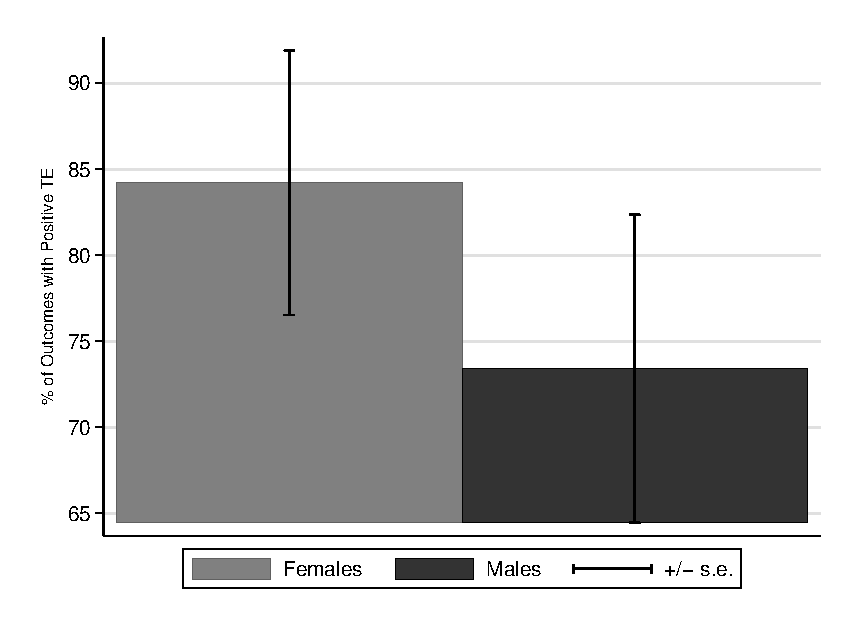
\includegraphics[width=\textwidth]{output/itt_noctrl_all.eps}
\end{subfigure}%
\begin{subfigure}[h]{0.4\textwidth}
	\centering
	\caption{Treatment vs. Next Best, Significant at 10\% Level} \label{fig:ppositive10}
		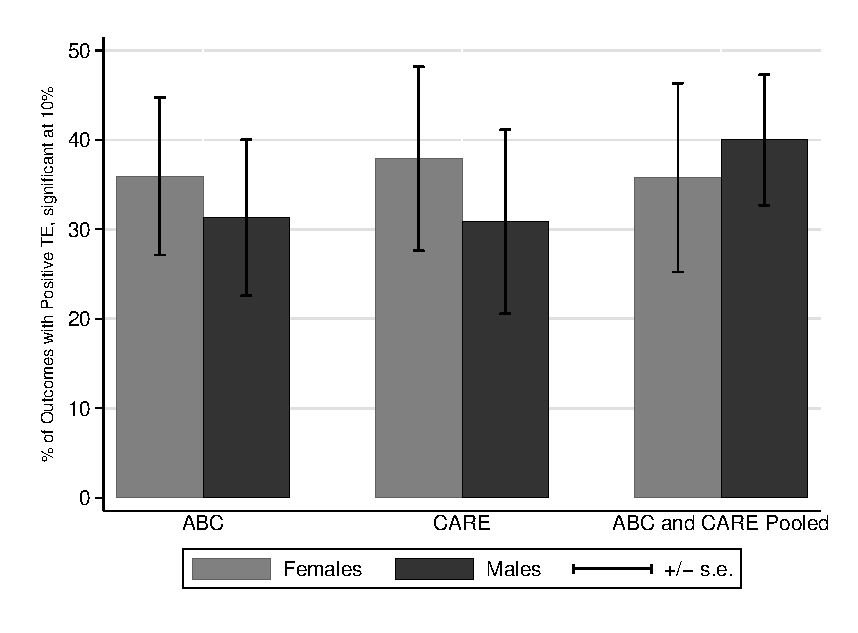
\includegraphics[width=\textwidth]{output/itt_noctrl_all_sig10.eps}
\end{subfigure}
\begin{subfigure}[h]{0.4\textwidth}
		\centering
		\caption{ Treatment vs. Stay at Home} \label{fig:ppositivehome}
		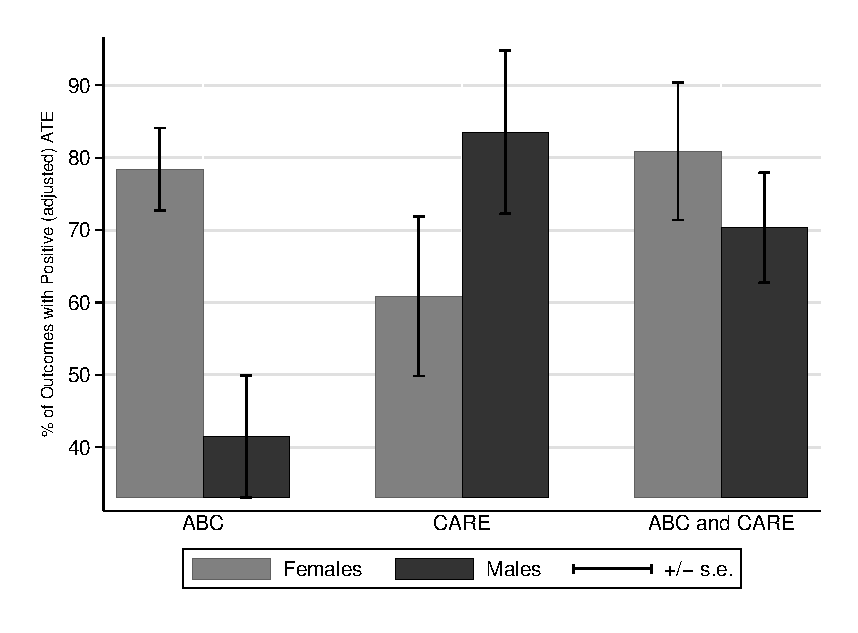
\includegraphics[width=\textwidth]{output/epan_ipw_p0_all.eps}
\end{subfigure}%
\begin{subfigure}[h]{0.4\textwidth}
	\centering
	\caption{Treatment vs. Alternative Preschool} \label{fig:ppositivealternative}
		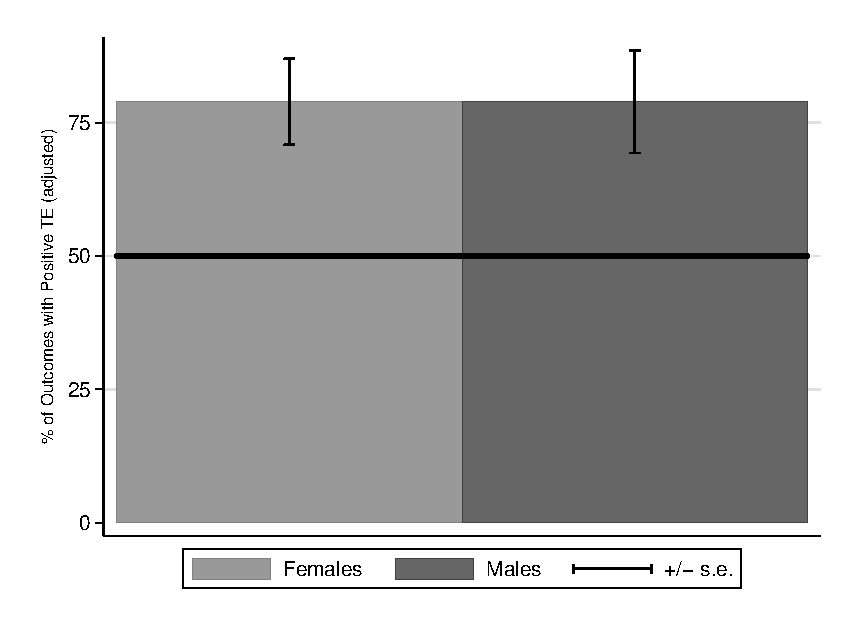
\includegraphics[width=\textwidth]{output/epan_ipw_p1_all.eps}
\end{subfigure}
\footnotesize \justify
Note: Panel (a) percentage of outcomes displaying a positive treatment effect, comparing treatment to next best. Panel (b) percentage of outcomes displaying a positive and significant treatment effect (10\% significance level). Panel (c) percentage of outcomes displaying a positive treatment effect, comparing treatment to staying at home. Panel (d) percentage of outcomes displaying a positive treatment effect, comparing treatment to alternative preschool. Standard errors are based on the empirical bootstrap distribution. For Panel (b) we perform a ``double bootstrap'' procedure to first determine significant treatment effects at $10\%$ level and then calculate the standard error of the count.\\
\end{sidewaysfigure}


\section{Predicting and Monetizing Life-cycle Costs and Benefits}\label{section:cbamethodology}

A central focus of this paper is on summarizing the multiple benefits of ABC/CARE using benefit/cost and rate of return analyses. This requires predicting the out-of-sample benefits of the program over the life cycle after the measurement phase of the study ends. This is a fundamental problem in empirical social science that has been addressed in the literature in multiple ways.\footnote{See, e.g., \cite{Heckman_Lochner_ea_2006_HEE}. \citet{Heckman_Moon_etal_2010_RateofReturn} use a variety of methods to project future labor income in the Perry study. The various methods are in general agreement. They fit a variety of panel data labor income dynamics models and project future labor income with them.} This section explains our strategy for using multiple data sources to extrapolate the life-cycle costs and benefits of education, labor income, transfer income, crime, and health. Our approach is motivated by the analysis of \citet{Heckman_Pinto_etal_2013_PerryFactor}, who show that the effect of treatment on outcomes operates through its effects of inputs in a stable production function rather than through shifts in the production function.

To construct cost-benefit estimates we (i) \textit{interpolate} components not observed due to intermittent data collection; and (ii) \textit{extrapolate} (predict) components not observed because the follow-ups stop when the subjects were in their mid-30s. We use multiple sources of non-experimental data representative on the national or state level to construct these interpolations and extrapolations. Table~\ref{table:sources} presents the components for which we conduct these exercises and the data sources we use. We use labor income as running example for illustration purposes, but our methodology is the same for predicting the rest of the outcomes unless otherwise noted.

\subsection{Using Auxiliary Samples to Predict Out of Sample}\label{sec:necrosis}

We have data on control- and treatment-group individuals through age $t^{\ast}$. We lack information on participant outcomes afterward. Yet, post-$t^{\ast}$ outcomes are required to construct counterfactual life-cycle profiles. The goal is to find counterparts to both treatment and control individuals in the auxiliary data on whom we have post-$t^{\ast}$ data.\footnote{An alternative approach to predict life-cycle income is to follow \citet{Mincer_1974_schooling}, who claims that labor income around $t^*$ is a good measure of lifetime income. We show that a discount rate of 2\% is necessary to equate a Mincer-type prediction to our life-cycle prediction in Appendix~\ref{app:mincer}.}

Because the participants of ABC/CARE are now in their mid-40s, there is no post-40s information on the same cohort  in any data. We use a synthetic cohort approach in which adjusted outcomes of older cohorts are used to estimate the future outcomes of the ABC/CARE participants. This approach is standard in the human capital literature. However, cohort effects may induce bias. We experiment with specifications that account for cohort effects when discussing our results in Section~\ref{section:cbaresults}.

\begin{table}[!htbp]
\begin{threeparttable}
\caption{Auxiliary Data Sources for Interpolation and Extrapolation of Life-cycle Benefits and Costs} \label{table:sources}
\footnotesize
%\input{../../AuxilliaryFiles/Preamble}
%\newgeometry{margin=.1in}

%\newcolumntype{L}[1]{>{\raggedright\let\newline\\\arraybackslash\hspace{0pt}}m{#1}}
%\newcolumntype{C}[1]{>{\centering\let\newline\\\arraybackslash\hspace{0pt}}m{#1}}
%\newcolumntype{R}[1]{>{\raggedleft\let\newline\\\arraybackslash\hspace{0pt}}m{#1}}

\begin{tabular}{L{3cm} C{1cm} C{1cm} C{1cm} C{1cm} C{1cm} C{2cm}} \toprule
 & \multicolumn{6}{c}{Subject's Age} \\
\textbf{Component}  & 16--21 & 21--30 & 31--34 & 34--50 & 61--67 & 68--Death \\ \midrule
\textbf{Transfer Income} & & \multicolumn{1}{c}{\cellcolor[gray]{.8} cNLSY} & \multicolumn{3}{c}{\cellcolor[gray]{.7} NLSY79; PSID}  &  \\ \midrule
\textbf{Subject Income} & &  \multicolumn{1}{c}{\cellcolor[gray]{.8} cNLSY} & \multicolumn{3}{c}{\cellcolor[gray]{.7} NLSY79; PSID} & \\ \midrule
\textbf{Health}  & \multicolumn{6}{c}{\cellcolor[gray]{.8} PSID; MEPS; MCBS; HRS}     \\ \midrule
\textbf{Crime} & \multicolumn{4}{c}{\cellcolor[gray]{.8} NCDPS; NJRP; NVS; UCRS} \\ \bottomrule
\end{tabular}
%\end{document}
\begin{tablenotes}
\footnotesize
Note: This table details the non-experimental data sources we use to interpolate and extrapolate the life-cycle benefits and costs of ABC/CARE. CNLSY: Children of the National Longitudinal Survey of the Youth 1979; NLSY79: National Longitudinal Survey of the Youth 1979; PSID: Panel Study of Income Dynamics; MEPS: Medical Expenditure Panel Survey; MCBS: Medicare Current Beneficiary Survey; HRS: Health and Retirement Study; NCDPS: North Carolina Department of Public Safety Data; NVS: National Crime Victimization Survey; NJRP: National Judicial Reporting Program; UCRS: Uniform Crime Reporting Statistics.
\end{tablenotes}
\end{threeparttable}
\end{table}

Following \citet{Heckman_Ichimura_etal_1998_REStud}, we use matching to find synthetic cohort counterparts in the auxiliary samples for both treatment and control group members. We match on baseline variables $\bm{B}$, as well as variables caused by treatment (for which there are treatment effects) that predict future outcomes---e.g., education, IQ, etc.---through age $t^{\ast}$. We then fit life-cycle relationships for outcomes beyond $t^{\ast}$ for the synthetic treatment and control groups using the initial conditions from the treatment and control groups at age $t^{\ast}$. From these predictions, we construct life-cycle profiles for the post-$t^*$ samples.

Specifically, let $\bm{Y}^{d}_{i,t}$ be an outcome at time $t$ for an individual in treatment status $d$. Measured predictors of the outcome are $\bm{X}^{d}_{i,t}$ and $\bm{B}_i$.\footnote{$\bm{B}$ is balanced across control- and treatment-group individuals by randomization.} We determine the predictors using within experimental sample analyses. We then find counterparts in the synthetic cohort samples. Let $S \in \{ 0,1\}$ denote membership in the experimental sample $(S=1)$ or the auxiliary sample $(S=0)$.

For individual $i$, find counterparts $j(i)$ for treatment and controls such that
\begin{equation}\label{eq:ingrownnail}
\sum_{j(i)\in F_0} \left( \bm{X}^{d}_{i,t} - \bm{X}_{j(i),t} \right)^{\prime} {\left( \bm{\Sigma}^d\right)}^{-1} \left(\bm{X}^{d}_{i,t} - \bm{X}_{j(i),t} \right) < \epsilon \text{ for } \qquad d \in \ \{0,1\}, t \in \{0,\dots,T\}
\end{equation}
where $\epsilon$ is arbitrarily small.\footnote{In practice, we set $\epsilon = 1$, but we try a range of values between .5 and 3 finding little sensitivity. The full set of the results we produce in the paper for multiple values in the interval [.5,3] is available under request.} $j(i) \in F_0$, for $t \leq t^{\ast}$, where $F_0$ is the index set in the auxiliary sample and $\bm{\Sigma}^d$ is the covariance matrix of the $\bm{X}$ in the experimental sample group $d$. We construct synthetic cohort samples using the same auxiliary samples and weight using the inverse value of~\eqref{eq:ingrownnail}. We fit dynamic relationships in the synthetic cohort sample over the whole sample period. Using the dynamic relationships in the synthetic cohort sample and the initial conditions from the experimental sample, we predict future outcomes. For this approach to produce unbiased forecasts, we require, among other things, that the support of the auxiliary sample includes the support of the experimental sample, an assumption formalized in the next subsection and tested in Appendix~\ref{app:containsupport}.\footnote{Evidence on this assumption is in Appendix~\ref{appendix:methodology}. In practice, we use indicators for black and male, year of birth, and years of education and labor income at age 30 as matching variables. We explain how we pick these variables and provide a sensitivity analysis to this choice in Appendix~\ref{appendix:methodology}.}

Figure~\ref{fig:labor-income-profiles} displays the life-cycle profiles for the synthetic control and treatment groups generated from this procedure.\footnote{We use labor income as an illustration in this section because the life-cycle patterns are well-known in the literature and straightforward to compare between the experimental and non-experimental samples. We predict transfer income using this same procedure. See Section~\ref{section:cbaresults} for results.} It also displays the profiles of the experimental control and treatment groups through $t^*$. The agreement through $t^*$ is close. The comparable profiles for females are in somewhat less agreement. Our pattern of life-cycle labor incomes is typical for low-skilled workers \citep{Blundell-etal_2015_J-Pub-E,Gladden_Taber_2000_WageProgression,Sanders-Taber_2012_AR,Lagakos_Moll_etal_2016_LifeCycle_NBER}.\footnote{The prediction is based on indicator variables of being male and being black, mother's education, average PIAT scores from ages 5 to 7, years of education at age 30, body-mass index at 34, labor income at ages 21 and 30, and one-period lagged labor income. We do not have all of the components of the High Risk Index in our auxiliary samples after age 45, so we only use a subset to make the life-cycle matches. A justification for the use of these variables, evidence on their predictive power, a sensitivity analysis to using different prediction variables are in Appendix~\ref{appendix:methodology}.}

\begin{sidewaysfigure}[!htbp]
\centering
\caption{Labor Income Profile Predictions}\label{fig:labor-income-profiles}
\begin{subfigure}[h]{0.5\textwidth}
		\centering
		\caption{Prediction for ABC/CARE Males} \label{fig:labor-income-profilesc}
		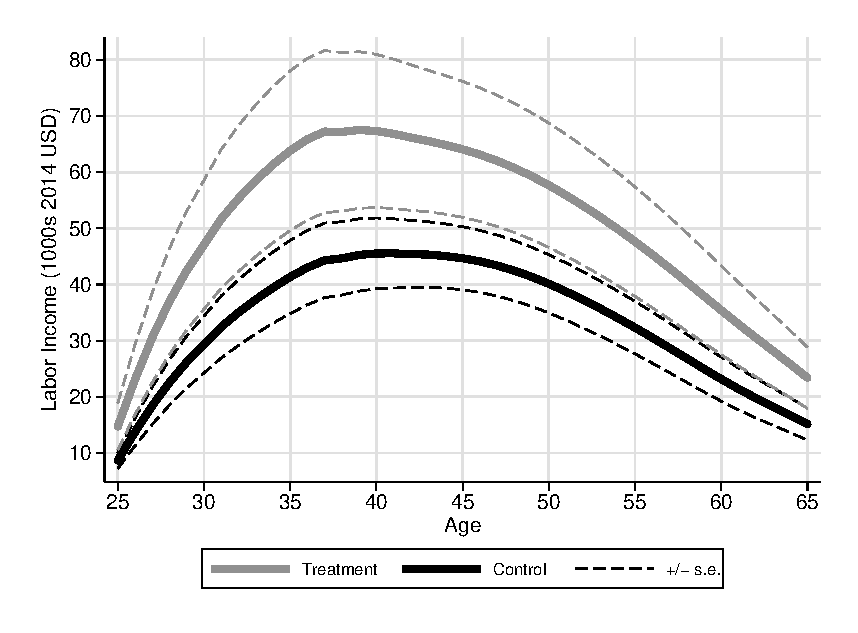
\includegraphics[width=\textwidth]{output/labor_25-65_pset1_mset3_male.eps}
\end{subfigure}%
\begin{subfigure}[h]{0.5\textwidth}
		\centering
		\caption{Prediction for ABC/CARE Females} \label{fig:labor-income-profilesa}
		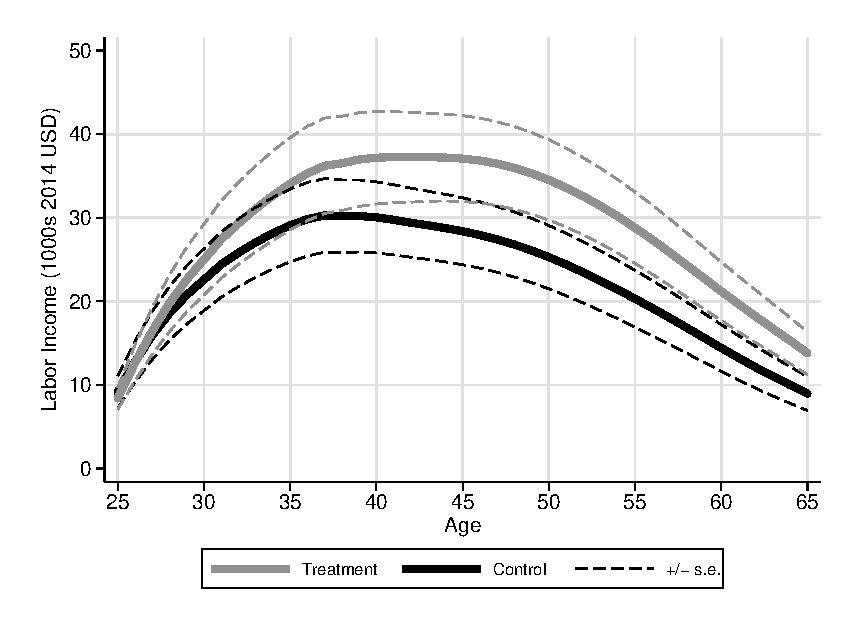
\includegraphics[width=\textwidth]{output/labor_25-65_pset1_mset3_female.eps}
\end{subfigure}
\footnotesize \justify
Note: Panels (a) displays the predicted labor income life-cycle profiles for ABC/CARE for males by treatment status, based on the method proposed in this section. We combine data from the Panel Study of Income Dynamics (PSID), the National Longitudinal Survey of Youth 1979 (NLSY79), and the Children of the National Longitudinal Survey of Youth 1979 (CNLSY79). We highlight the \textit{realized or observed} labor income at $t^*$ (age 30) for the ABC/CARE control- and treatment-group participants. Panel (b) displays the analogous figure for females. Standard errors are based on the empirical bootstrap distribution.  See Appendix~\ref{appendix:methodology} for a discussion of our choice of predictors and a sensitivity analysis to this choice.
\end{sidewaysfigure}

In the experimental sample, all of the parents of children with observed characteristics $\bm{B} \in \mathcal{B}_0$ agree to participate in the program. Since in the non-experimental sample there are no treatment group members, a test of the validity of our matching procedure is to compare the labor incomes of individuals in the non-experimental sample for whom $\bm{B} \in \mathcal{B}_0$ to the labor incomes of the synthetic control group members (i.e., the groups in the non-experimental samples that we use to extrapolate control group outcomes). We also compare labor income at $t^*$ of both groups to the observed labor income in the experimental control group (we observe labor income at $t^*$). Figure~\ref{figure:controltests} makes these comparisons. We plot the labor income of individuals in our non-experimental sample such that $\bm{B} \in \mathcal{B}_0$ and the synthetic control group from ages 20 to 45. We also display the labor income of the experimental control group at $t^*$ (age 30).\footnote{The graphs stop at age 45 because we do not observe all of the components of the High Risk Index after age 45 in the non-experimental samples. We use only a subset of it to make our life cycle projections. The subset variables are effective predictors over the range where the full set of $\bm{B}$ is available.}

\begin{sidewaysfigure}[!htbp]
\centering
\caption{Labor Income Profile, Disadvantaged Individuals Synthetic Control Group in the Non-experimental Samples}\label{figure:controltests}
\begin{subfigure}[h]{0.5\textwidth}
		\centering
		\caption{Males}
		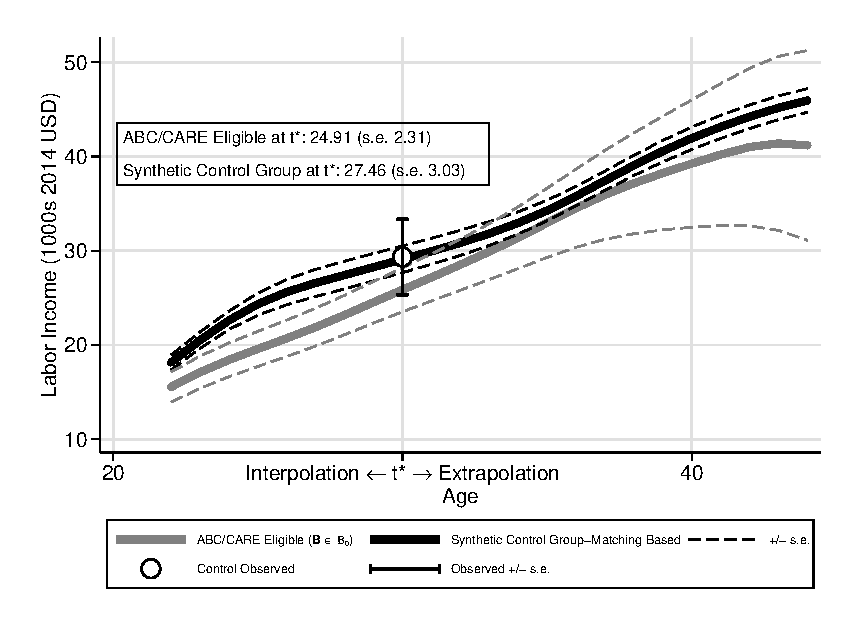
\includegraphics[width=\textwidth]{output/abccare_disad_1.eps}
\end{subfigure}%
\begin{subfigure}[h]{0.5\textwidth}
		\centering
		\caption{Females}
		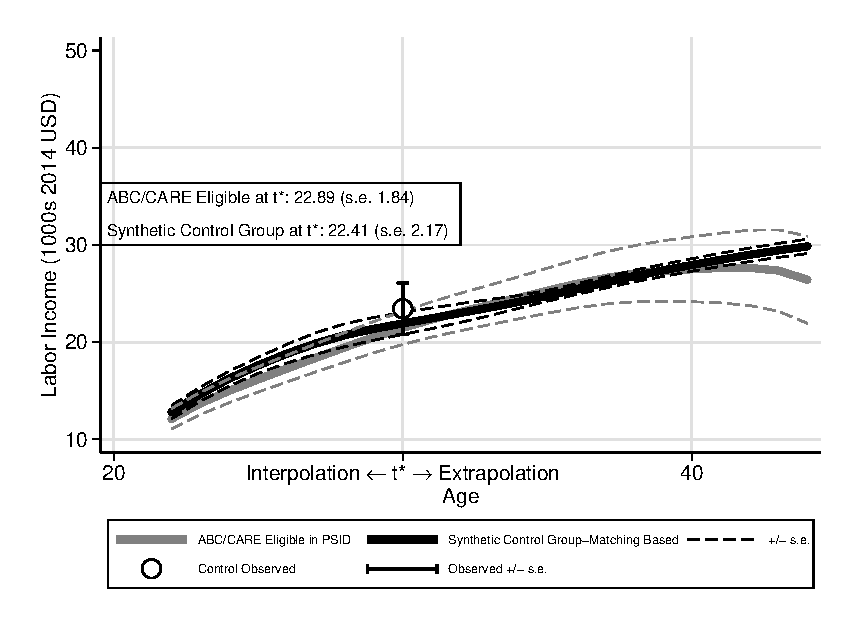
\includegraphics[width=\textwidth]{output/abccare_disad_0.eps}
\end{subfigure}
\footnotesize \justify
Note: Panels (a) displays the predicted labor income for males in the non-experimental samples such that $\bm{B} \in \mathcal{B}_0$, i.e. ABC/CARE eligible, and for the synthetic control group we construct based on the method proposed in this section. We combine data from the Panel Study of Income Dynamics (PSID), the National Longitudinal Survey of Youth 1979 (NLSY79), and the Children of the National Longitudinal Survey of Youth 1979 (CNLSY79). We highlight the \textit{realized or observed} labor income at $t^*$ (age 30) for the ABC/CARE control- and treatment-group participants. We stop at age 45 for want of data to compute the high-risk index defining $\bm{B} \in \mathcal{B}_0$ in ABC/CARE in the non-experimental samples. Panel (b) displays the analogous figure for females. Standard errors are based on the empirical bootstrap distribution.
\end{sidewaysfigure}

\subsection{Justifying the Matching Procedure} \label{section:just}

To examine the conditions for the validity of the matching approach, and to provide an analytical framework for the extrapolations used in this paper, it is helpful to introduce some general notation. Recall that $\bm{Y}^d_{j,t}$ is outcome $j$ at time $t$ for person fixed to $(d\in\{0,1\})$. To simplify the analysis, in this subsection we do not further partition the control group. We define determinants of outcomes---vector $\bm{X}^d_t$---that may themselves be the outcomes of treatment, and may also depend on lagged outcomes also affected by treatment. Outcome variables are generated by the following equation

\begin{equation}\label{eq:trenchfoot}
\bm{Y}^d_{j,t} = \phi^d_{j,t} (\bm{X}^d_t, \bm{B}, \varepsilon^d_{j,t}), \quad d \in \{0,1\}, \quad \  j \in \mathcal{J}_t, t \in \{0,\dots,T\}
\end{equation}

\noindent where $\mathcal{J}_t$ is the index set of possible outcomes and $\varepsilon^d_{j,t}$ is a scalar unobserved determinant of $\bm{Y}^d_{j,t}$. $\bm{Y}^d_{t-1}$ can be included among the $\bm{X}^d_{t}$. 

We estimate first order Markov relationships for labor income, parental income, transfer income, and health. The equation of motion for determinant $k \in \mathcal{K}_t$ (the set of determinants at time $t$) is given by

\begin{equation}\label{eq:frostbite}
\bm{X}^d_{k,t} = \gamma^d_{k,t} (\bm{X}^d_{t-1}, \bm{B}, \eta^d_{k,t}), \quad d \in \{0,1\}, \ k \in \mathcal{K}_t, t \in \{0,\dots,T\}
\end{equation}

\noindent where $\eta^d_{k,t}$ is an unobserved determinant of $\bm{X}^d_{k,t}$. The $\bm{X}^d_{k,t}$ can be caused by treatment, as can $\bm{X}^d_{t-1}$. Examples of $\bm{X}^d_t$ in our data are education, IQ, health, work experience, and participation in crime. All are potential determinants of labor income.

We assume \emph{structural invariance} of \eqref{eq:trenchfoot} and \eqref{eq:frostbite}.\footnote{See, e.g., \citet{Frisch_1938_autonomy}, \citet{Haavelmo_1943_Econometrica,Haavelmo_1944_Econometrica}, \citet{Hurwicz_1962_structural}, and \citet{Heckman_Pinto_2015_EconometTheory}.} This means that however the arguments of \eqref{eq:trenchfoot} and \eqref{eq:frostbite} are determined, for the same numerical values of $(\bm{X}^d_t, \bm{B}, \varepsilon^d_t)$ and $(\bm{X}^d_{t-1}, \bm{B}, \eta^d_{j,t})$, we obtain the same values of $\bm{Y}^d_{j,t}$.\footnote{Frisch called this notion ``autonomy.'' Much later work in statistics captures structural invariance as one aspect of ``SUTVA.'' See \citet{Holland_1986_JASA} and \citet{Heckman_2008_ISR}.} This is a fundamental property of invariant economic relationships used by economists since the time of \citet{Frisch_1938_autonomy}.

\onehalfspacing
\begin{assumption}\label{ass:butts}: \textbf{Structural Invariance} \\
\noindent Fixing $\bm{X}^d_t = (\bm{x}_t, b,\bar{\varepsilon}_t)$, $y^d_{j,t} = \phi^d_{j,t} (\bm{x}_t, b,  \bar{\varepsilon}^d_{j,t})$ for $j \in \mathcal{J}_t$ and $t \in \{0,\ldots,T\}$ takes the same value as $\bm{Y}^d_{j,t}$ when $\bm{X}^d_{t-1} = \bm{x}_t$, $\bm{B} = b$, and $\varepsilon^d_{j,t} = \bar{\varepsilon}_{j,t}$. Fixing $\bm{X}^d_{t-1} = (x_{t-1}, b, \bar{\eta}_t)$, $\bm{X}^d_{k,t} = \gamma^d_{k,t} (x_{t-1}, b, \bar{\eta}_t)$ for $k \in \mathcal{K}_t$ and and $t \in \{0,\ldots,T\}$ takes the same values as $\bm{X}^d_{k,t}$ when  $\bm{X}^d_{k,t-1} = x_{t-1}$, $\bm{B} = b$, and $\eta^d_t = \bar{\eta}_t, t \in \{0,\dots,T\}$.
\end{assumption}
\doublespacing

Equations~\eqref{eq:trenchfoot} and \eqref{eq:frostbite} can be estimated in the sample period $\left(0,\ldots,t^{*}\right]$. We do not observe data on the experimental sample after $t^{*}$. To predict outside the sample period, we access auxiliary data on older cohorts of individuals whose life-cycle equations of motion are governed by Equations~\eqref{eq:trenchfoot} and \eqref{eq:frostbite}. This presumes the absence of cohort effects. We discuss the validity of this assumption when we turn to our empirical estimates.

\onehalfspacing
\begin{assumption}\label{ass:crotchrot}
\textbf{Absence of Cohort Effects}
\end{assumption}
\doublespacing

Our auxiliary data do not have direct information on program participation. However, given the limited size of the experimental sample, and the fact that the auxiliary cohorts were not eligible to participate in the program, it is reasonable to assume that no one in the auxiliary sample is treated ($D=0$). This means that \eqref{eq:trenchfoot} and \eqref{eq:frostbite} for $d=0$ can be identified over the supports of the available samples in the post-sample period. This implies that we can identify the post-experimental outcomes for the ABC/CARE control groups if the supports of the auxiliary data includes the support of the experimental data.

Using somewhat imprecise, but self-evident notation, $\bm{Y}_j = (\bm{Y}^1_j, \bm{Y}^0_j)$, $\bm{X}_l = (\bm{X}^1_l, \bm{X}^0_l)$, $\bm{\varepsilon}_n = (\bm{\varepsilon}^1_n, \bm{\varepsilon}^0_n)$, and define $\bm{X}^s = (\bm{X}_0,\dots,\bm{X}_T)^s$, $\bm{B}^s$, $\bm{Y}^s = (\bm{Y}_0,\dots,\bm{Y}_T)^s$, $\bm{\varepsilon}^s = (\bm{\varepsilon}_0,\dots,\bm{\varepsilon}_{T})^s$ where $s$ denotes sample membership. We assume:

\onehalfspacing
\begin{assumption} \label{ass:contain} \textbf{The support of the auxiliary sample contains the support of the experimental sample:}
\begin{equation*}
\sup(\bm{X}, \bm{Y}, \bm{B}, \varepsilon)^{s=1} \subseteq \sup (\bm{X}, \bm{Y}, \bm{B}, \varepsilon)^{s=0}.
\end{equation*}
\end{assumption}
\doublespacing 

In particular, we assume that the support of $\mathcal{B}_0$ is included in the auxiliary sample.\footnote{Evidence in support~\eqref{ass:contain} is presented in Appendix~\ref{app:containsupport}.} Predicting treatment group outcomes is a more challenging task. We do so by invoking the assumption that outcome equations \eqref{eq:trenchfoot} and \eqref{eq:frostbite} are the same across treatment and control regimes. Formally, we assume

\onehalfspacing
\renewcommand\theassumption{A--\arabic{assumption}(a)}
\begin{assumption}\label{ass:eczema}
\textbf{For any} $\bm{X^d_t}, \bm{B}, \bm{\varepsilon^d_{j,t}}$ \textbf{in} $\bm{\sup}(\bm{X},\bm{Y},\bm{B})^{s=1}$,
\begin{equation*}
\phi^1_{j,t} (\bm{X}^d_t, \bm{B}, \varepsilon^d_{j,t}) = \phi^0_{j,t} (\bm{X}^d_t, \bm{B}, \varepsilon^d_{j,t}) \qquad j \in \mathcal J_t, \quad t \in \{0,\dots,T\},
\end{equation*}
\end{assumption}
\doublespacing

i.e., treatment effects operate through inputs and not shifts in the input-output functions. This allows us to use post-$t^*$ relationships fit on the auxiliary samples to forecast post-$t^*$ outcomes of treatment group members. Evidence for the validity of this assumption in the context of early childhood programs is presented in \citet{Heckman_Pinto_etal_2013_PerryFactor} and \citet{Attanasio-etal_2015_NBER_Estimating-Production}. In Appendix~\ref{app:invariance}, we test and do not reject this assumption for parental income, labor income, and transfer income using the factor structure control function approach developed in \citet{Heckman_Pinto_etal_2013_PerryFactor}.

We make a corresponding assumption for the equation governing the evolution of inputs:

\addtocounter{assumption}{-1}
\renewcommand\theassumption{A--\arabic{assumption}(b)}
\onehalfspacing
\begin{assumption}\label{ass:psoriasis}
\textbf{Given} $\bm{X^d_{t-1}}, \bm{B}, \bm{\eta^d_{l,t}}$,
\begin{equation*}
\gamma^1_{j,t} (\bm{X}^d_{t-1}, \bm{B}, \eta^d_{t-1}) = \gamma^0_{j,t} (\bm{X}^d_{t-1}, \bm{B}, \eta^d_{t-1}) \qquad k \in \mathcal{K}_t, \quad t \in \{0,\dots,T\}.
\end{equation*}
\end{assumption}
\doublespacing
We assume that the $\bm{X}^d_t$ are exogenous with respect to the errors:

\renewcommand\theassumption{A--\arabic{assumption}}
\onehalfspacing
\begin{assumption}\label{ass:corns} \textbf{Exogeneity}
\begin{equation*}
\bm{\varepsilon}^d_{j,t} \indep \bm{X}^{d^{\prime}}_{t^{''}} \quad \forall \; t,t^{''} \in \left[ 0,...,T \right], d,d^{\prime} \in \left\{ 0,1 \right\}, \; \forall \quad j \in \mathcal{J}_t, \quad t \in \left\{0,\dots,T\right\}
\end{equation*}
\end{assumption}
\doublespacing
\noindent in sample $S=1$ and the counterpart assumption in $S=0$.

\onehalfspacing
\begin{theorem}
Putting Assumptions~\ref{ass:butts} through \ref{ass:corns} together, under full observability of $\bm{X}^d_t$, estimation on the matched samples based on \eqref{eq:ingrownnail} generates unbiased out of sample treatment effects.\footnote{See the analysis of \citet{Heckman_Navarro_2004_REStat}, who discuss the central role of exogeneity assumptions in matching.} $\Box$ The proof is straightforward.
\end{theorem}
\doublespacing

Our predictions are based on matching individuals in the non-experimental sample to individuals in the experimental samples \textit{on the basis of observed characteristics}. In general, the dependence between $\bm{X}_{t}$ and $\bm{\varepsilon}_{t}$ is not the same across those two samples. Assumption~\eqref{ass:corns} may be violated in either sample. Such violations can arise in two ways: (i) the experiment does not necessarily identify the production function in \eqref{eq:trenchfoot} because there could be unmeasured inputs (generated by the experiment not fully captured by the measured variables and (ii) even if we can measure all inputs, the inputs may not be exogenous in the non-experimental sample.

A simple example is the following: in the treatment sample, the program causes more education. Suppose we match based on education to create a treatment synthetic cohort. But doing so, we may match individuals in the non-experimental sample who are highly educated because they come from better backgrounds and are more motivated compared to those in the experiment who are induced to be educated by the experiment. Omitted ability could bias predictions based on the matched samples.

We discuss these issue and present a comprehensive set of tests of Assumption~\ref{ass:eczema} and Assumption~\ref{ass:corns} in Appendix~\ref{appendix:methodology}. Here we present a brief discussion of the methodology for doing so and illustrate it presenting tests for Assumption~\ref{ass:eczema}. 

A potential problem is endogeneity (e.g., mean dependence between schooling years and unobserved skills). Unless the bias in the treatment and control groups are exactly the same, endogeneity would bias our predictions. If predictions are linear, a sufficient condition to obtain unbiased predictions is $\mathbb{E} \left[ \bm{\varepsilon}_{j,t}^0 | \bm{X}_{t}^d, \bm{B} \right] = \mathbb{E} \left[ \bm{\varepsilon}_{j,t}^1 | \bm{X}_{t}^d, \bm{B} \right]$. 

An alternative is to follow \citet{Heckman_Pinto_etal_2013_PerryFactor} and obtain an approximation for  $\bm{\varepsilon}_{j,t}^d$ based on a measurement system. Formally, let the system be

\begin{eqnarray}
\bm{M}_{t}^d     &=& \bm{\lambda}^d \bm{\theta}_{t}^d +  \bm{\upsilon}_t^d, \text{ where } \bm{\theta}^d  \independent \bm{\upsilon}_{t}^d \ \forall t \\ \nonumber
\bm{\varepsilon}_{t}^d &=& \bm{\beta}^d \bm{\theta}_{t}^d + \bm{\omega}_{t}^d \text{ where } \bm{\theta}^d  \independent \bm{\omega}_{t}^d \ \forall t \\ \nonumber
&\upsilon_{t}^d \independent \omega_{t}^d.
\label{eq:msystemmain}
\end{eqnarray}

With an auxiliary system of measures such that $\bm{M}_{t}^d $ has at least three elements, we are able to identify the vectors of coefficients characterizing these system: $\bm{\lambda}^d, \bm{\beta}^d$, as well as the respective covariance matrices $\Sigma_{\bm{\theta}_{t}^d}, \Sigma_{\bm{\upsilon}_{t}^d}$, and use the method in \citet{Bartlett_1938_Nature} to obtain an estimate of $\bm{\theta}_{t}^d$ \citep{Cunha_Heckman_ea_2005_oep,Cunha_Heckman_etal_2010_est_tech_cognoncog}. To put this in practice, we assume that $\bm{\theta}_{t}^d$ has two dimensions (one representing cognitive skill, $c$, and another representing non-cognitive skill, $n$). We assume dedicated measures for these skills at one time period. Put simply, we have two independent systems, one to measure $\bm{\theta}_{c}^d$ and one to measure $\bm{\theta}_{n}^d$, where $\bm{\theta}_{t}^d: = \left[ \bm{\theta}_{c}^d, \bm{\theta}_{n}^d \right]$. Further, we assume a common measurement system for the treatment and control groups (this is a sensible assumption given the small size of our sample). This assumption implies that $\bm{\lambda}^d, \bm{\beta}^d$, as well as $\bm{\Sigma}_{\bm{\theta}_{t}^d}, \bm{\Sigma}_{\bm{\upsilon}_{t}^d}$ are the same either when $d = 0$ or when $d = 1$.

We use a set of measures from ages 2 to 8 to to obtain an estimate of $\bm{\theta}_{c}^d$ and a set of measures of somatization, hostility, depression, and global index of mental health to measure (all at age 21) to estimate $\bm{\theta}_{n}^d$.\footnote{For definitions and treatment effects on these variables see Appendix~\ref{appendix:results}.} Figure~\ref{figure:factorsm} shows our estimates by treatment status.

\begin{figure}[H]
\centering
\caption{Estimates of Cognitive ($\theta_{c}^d$) and Non-cognitive Skills ($\theta_{n}^d$)}\label{figure:factorsm}
\begin{subfigure}[h]{0.5\textwidth}
		\centering
		\caption{Cognitive} \label{fig:c}
		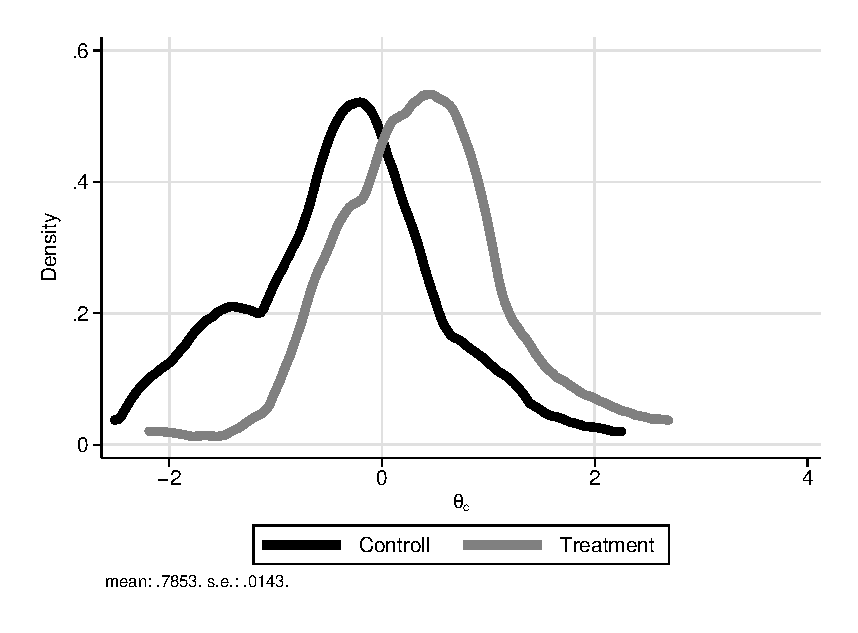
\includegraphics[width=\textwidth]{output/abccare_cfactor.eps}
\end{subfigure}%
\begin{subfigure}[h]{0.5\textwidth}
	\centering
	\caption{Non-cognitive} \label{fig:n}
		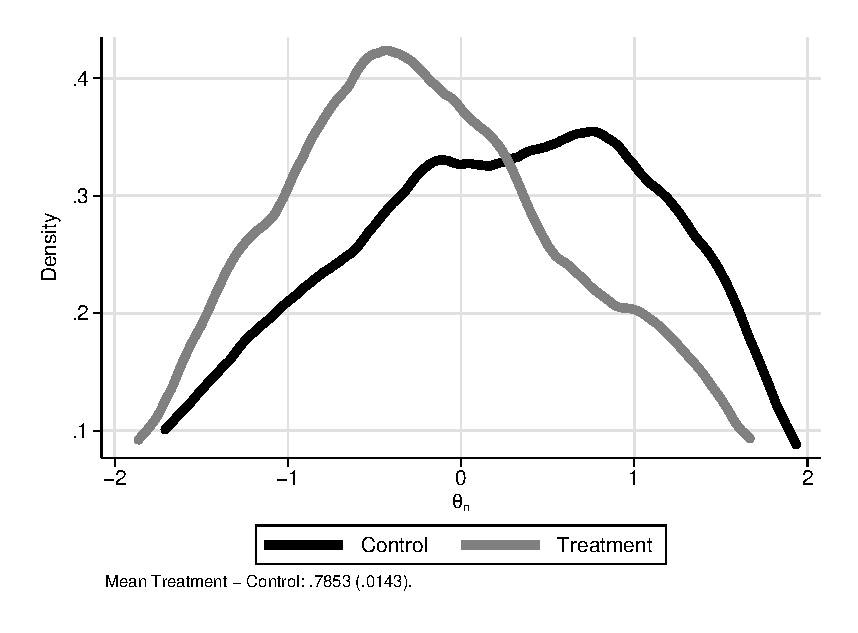
\includegraphics[width=\textwidth]{output/abccare_nfactor.eps}
\end{subfigure}
\footnotesize \justify
Note: Panels (a) displays a factor score estimated based on the measurement system in \eqref{eq:msystem} and measures of IQ at ages 2, 3, 4, 5, 7, and 8 (cognitive skill). Panel (b) displays an analogous exercise using measures measures of somatization, hostility, depression, and a global mental health index at age 21 (non-cognitive skill). Both measures of skills are standardized to a mean of $0$ and a standard deviation of $1$. The mean difference between treatment and control is displayed below each panel, with standard error in parentheses. Standard errors are based on the bootstrap empirical distribution.
\end{figure}

Given the conditions in \eqref{eq:msystemmain}, the estimated coefficients characterizing \eqref{eq:eqs} are unbiased, and therefore we can test Assumption~\ref{ass:eczema}. The tests consists of asking if the predictions variables we use are enough to summarize the treatment effects on the variables we predict, and therefore an indicator of treatment take-up becomes irrelevant when conditioning on these variables. We cannot reject the hypothesis that coefficient associated to random assignment to treatment is different from zero, once we condition on the variables we use to predict (see Table~\ref{table:testing}). Using this same structure, we propose tests for Assumption~\ref{ass:corns} in Appendix~\ref{appendix:methodology}. We do not find strong evidence against it.

\begin{table}[!htbp]
\begin{threeparttable}
\caption{Testing Assumption~\ref{ass:eczema}, ABC/CARE}\label{table:testing}
\scriptsize
\begin{tabular}{lcccccc}
\toprule
& \multicolumn{2}{c}{Parental Income} & \multicolumn{2}{c}{Labor Income} & \multicolumn{2}{c}{Transfer Income}\\
\midrule
$R$ & 4,804.658 & 7,577.495 & -5,730.742 & -7,247.364 & -2,135.622 & -2,647.890 \\
& (0.275) & (0.135) & (0.855) & (0.820) & (0.915) & (0.900) \\
Mother's Education & -305.154 & 1,121.884 & -3,318.864 & -3,832.640 & -62.241 & -60.393 \\
& (0.570) & (0.265) & (0.915) & (0.910) & (0.560) & (0.530) \\
PIAT (5--7) & 416.503 & -262.980 & 127.141 & 176.826 & -55.700 & -118.258 \\
& (0.155) & (0.645) & (0.370) & (0.410) & (0.850) & (0.845) \\
Education (30) & -171.016 & -1,413.658 & 10,252.614 & 12,651.459 & -455.730 & -431.236 \\
& (0.530) & (0.685) & (0.010) & (0.010) & (0.890) & (0.780) \\
Labor Income (21) & -0.002 & 0.085 & 0.238 & 0.237 & -0.111 & -0.142 \\
& (0.500) & (0.445) & (0.160) & (0.300) & (0.980) & (0.985) \\
BMI (34) & -93.408 & -39.170 & -289.772 & -320.442 & 4.293 & 3.892 \\
& (0.625) & (0.580) & (0.880) & (0.865) & (0.475) & (0.480) \\
$\hat{\bm{\theta}}_c$ &   & 4,879.198 &   & -2,587.188 &   & 468.628 \\
&  &  (0.140) &   & (0.665) &   & (0.360) \\
$\hat{\bm{\theta}}_n$ &   & 8,518.073 &   & 4,328.802 &   & -268.582 \\
&   & (0.025) &   & (0.205) &   & (0.620) \\
Constant & -8,751.849 & 52,407.562 & -69,100.00 & -95,900.00 & 16,758.146 & 23,489.504 \\
& (0.595) & (0.235) & (0.975) & (0.955) & (0.035) & (0.055) \\ \\
\midrule
$F$-stat & 2.728 & 6.048 & 4.208 & 3.796 & 2.879 & 2.930 \\
$R^2$ & 0.219 & 0.502 & 0.348 & 0.444 & 0.223 & 0.288 \\
Observations & 40 & 35 & 76 & 61 & 75 & 61 \\
\bottomrule
\end{tabular}
\begin{tablenotes}
\scriptsize
\item Note: This table presents results from regressing the different outcomes we predict on the predicted variable, proxies for the unobserved variables, and randomizes assignment to treatment in ABC/CARE ($R$). Empty cells indicate that the variable was not used in the prediction. $\hat{\bm{\theta}}_{c}$: factor score estimated based on the measurement system in \eqref{eq:msystemmain} and measures of IQ at ages 2, 3, 4, 5, 7, and 8 (cognitive skill). $\hat{\bm{\theta}}_{n}$: factor score estimated based on the measurement system in \eqref{eq:msystem} and measures of somatization, hostility, depression, and a global mental health index at age 21 (non-cognitive skill). Both measures of skills are standardized to a mean of $0$ and a standard deviation of $1$. Inference is based on the empirical bootstrap distribution and one-sided $p$-values are in parentheses. If the estimates for the constant terms are in the ten or hundred thousands, we report a figure that has been rounded to the thousands.
\end{tablenotes}
\end{threeparttable}
\end{table}


 \textbf{[JJH: Jorge, do we do this in comparison samples? Where?] [JLG: yes, noting the appendix after assertion now. And they effectively do not change in either the experimental or non-experimental samples.] [JJH: Give me updated figure.] [JLG: All tables with these tests in Appendix C.6.] [JJH: No shift in intercept actually? Seems too strong -- yet we need it.]  [JLG: Yes, we cannot reject differences once we account for all our prediction variables.] [JLG: I'm coordinating with Rodrigo for this on Perry. Not for him to do it, but for me to use the same measures that you use in the AER paper.]}

\subsection{Parental Income} \label{section:pincome}

In practice, ABC/CARE had a childcare component: child care of the mothers of parents of treated children was offered at the center for more than nine hours a day for five years. Recall that only $27\%$ of mothers of children reported to live with a partner at baseline and this status barely changed during the experiment (See Appendix~\ref{appendix:background}). Arguably, this is the component that generates the treatment effects in maternal education, labor force participation, and parental income that reported in Table~\ref{table:tescombined} and Appendix~\ref{appendix:results}.

We observe parental income at eight different years from when the experimental subjects were born until they were 21.\footnote{The ages at which parental income is absorbed is at ages 0, 1.5, 3.5, 4.5, 8, 12, 15, and 21. At age 21 the mothers in ABC/CARE are, on average, 41 years old.} Our baseline estimation considers the treatment effect on parental income without going beyond this age. We linearly interpolate the ages for which we do not have observations between 0 and 21.\footnote{Depending on the model of labor supply, labor income should or should not include the value of forgone leisure. We conduct a sensitivity analysis below by considering the case when markets are assumed to be clearing and the marginal value of leisure is the market wage.} As Table~\ref{table:tescombined} shows, treatment effects on parental income are sustained through child's age 21. This is presumably due to wage growth due to higher education and/or experience. An ideal approach considers the profile over the full life cycle of mothers. We propose two alternative approaches for doing this in Appendix~\ref{app:parentalincome}: (i) an approach based on parameterizing parental labor income using standard Mincer equations; (ii) an approach based on the model of Section~\ref{section:just}. We present estimates using the baseline approach and for these two alternatives in Section~\ref{section:cbaresults}. The benefits of he program increase when considering the full life cycle of mothers, in either approach.

Note that if it is true that ABC/CARE had a childcare component benefits parental labor market outcomes, it is likely the case that it benefits parents who, at baseline, did not have any other children. If they did, then they might have had to take care of other children anyway, weakening the childcare-driven effect (especially if there are younger siblings present). Figure~\ref{figure:pincome} shows that the net increase (treatment minus control) in discounted parental incomes is much higher in the absence of siblings (of the participant children) at baseline. The effect also weakens when comparing children who have children younger than 5 years old to children who have siblings 5 years old or younger.\footnote{These patterns persist when splitting the ABC/CARE sample by gender, but the estimates are not precise because the samples become to small when we split them.}

\begin{figure}[!htbp]
\centering
\caption{Discounted Parental Income by Participant's Number and Age of Siblings at Baseline}\label{figure:pincome}
\begin{subfigure}[h]{0.5\textwidth}
		\centering
		\caption{No Siblings vs. $>0$ Siblings}
		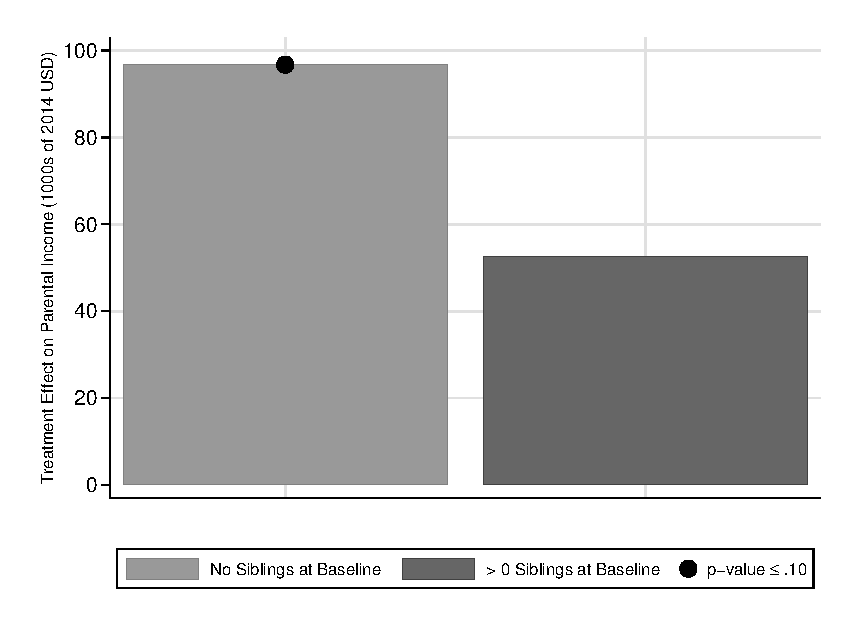
\includegraphics[width=\textwidth]{output/abccare_pincomesum_spooled.eps}
\end{subfigure}%
\begin{subfigure}[h]{0.5\textwidth}
		\centering
		\caption{Siblings Younger than 5 vs. Siblings 5 or Older}
		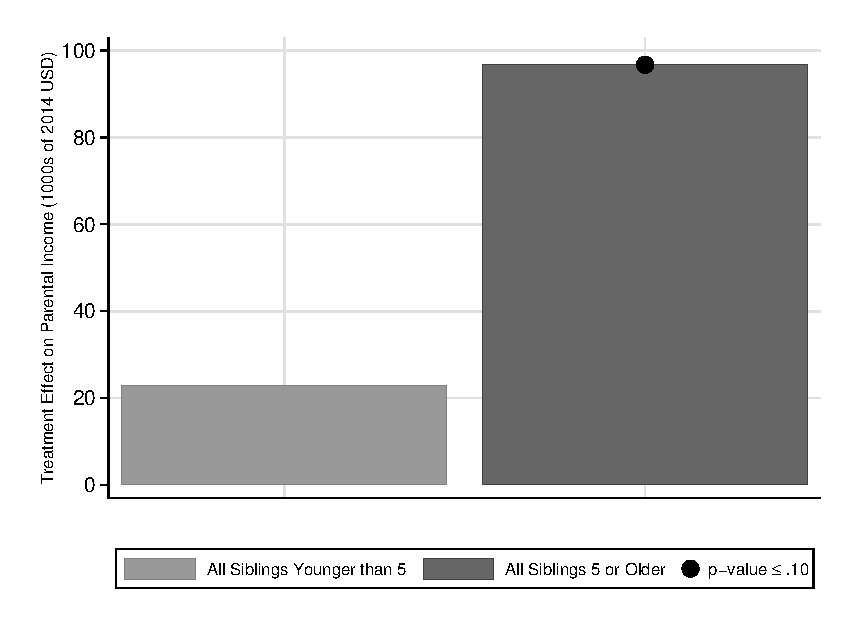
\includegraphics[width=\textwidth]{output/abccare_pincomesumsibage_spooled.eps}
\end{subfigure}
\footnotesize \justify
Note: Panel (a) displays the average parental income of parents of children with and without siblings at baseline. Panel (b) displays the average parental income of parents of children with young siblings (younger than 5 years old) and children with older siblings (5 years old or older) at baseline. Panel (b) drops children without siblings at baseline. Parental income is in 2014 USD discounted to child's participant age 0. We use the baseline measure of parental income in Section~\ref{section:pincome}. Results using our alternative parental income measures are similar (see Appendix~\ref{app:parentalincome}).
\end{figure}

\subsection{Health} \label{section:health}

 We predict and monetize health outcomes based on a version of Equation~\eqref{eq:trenchfoot} with a full vector of lagged dependent variables. This requires adapting the the models of Section~\ref{section:just}. Three additional issues arise: (i) health outcomes such as diabetes or heart disease are absorbing states; (ii) health outcomes are highly interdependent within and across time periods; and (iii) there is no obvious terminal time period for benefits and costs except death, which is endogenous.\footnote{For example, for income we extrapolate up to the retirement age of 67. However, for health, we need to predict an age of death for each individual.} Our auxiliary model for health is an adaptation of the Future America Model (FAM). This model predicts health outcomes from the subjects' mid-30s up to their projected death \citep{Goldman_etal_2015_Future-Elderly-Model-Report}.\footnote{The simulation starts at the age in which we observe the subject's age-34 health follow-up. On average this happened at age 34 for both males and females, but there is variation ranging from age 30 to age 37.} Appendix~\ref{appendix:health} discusses the FAM methodology in detail. We initialize the health prediction using the same variables that we use when predicting labor and transfer income, along with the initial health conditions as listed in Table~\ref{table:transition}.

The methodology has five steps: (i) estimate age-by-age health state transition probabilities using the Panel Study of Income Dynamics (PSID); (ii) match these transition probabilities to the ABC/CARE subjects based on observed characteristics; (iii) estimate quality-adjusted life year (QALY) models using the Medical Expenditure Panel Survey (MEPS) and the PSID; (iv) estimate medical cost models using the MEPS and the Medicare Current Beneficiary Survey (MCBS), allowing estimates to differ by health state and observed characteristics; and (v) predict the medical expenditure and QALYs that correspond to the simulated individual health trajectories.\footnote{As an intermediate step between (i) and (ii), we impute some of the variables used to initialize the FAM models (see Appendix~\ref{appendix:health}).}

Our microsimulation model starts the health predictions at age 30, with the information on observed characteristics available at this age. Restricting it to the individuals for whom we have information from the age-34 health follow-up allows us to account for components that are important for predicting health outcomes, such as the body mass index (BMI) and measures of diastolic and systolic blood pressure readings. The models predict the probability of being in any of the states in the horizontal axis of Table~\ref{table:transition} at age $a+1$ based on the state at age $a$, which is described by the vertical axis of the table.\footnote{In practice, the predictions are based on two-year lags, due to data limitations in the auxiliary sources we use to simulate the FAM. For example, if the individual is 30 (31) years old in the age-30 interview, we simulate the trajectory of her health status at ages 30 (31), 32 (33), 34 (35), and so on until her projected death.} Absorbing states are an exception. For example, heart disease at age $a$ does not enter in the estimation of transitions for heart disease at age $a+1$ because it is an absorbing state: once a person has heart disease, she carries it through the rest of her life.

\begin{sidewaystable}[!htbp]
\begin{threeparttable}
\caption{Health State Transitions, Age $a$ as Predictor of Age $a+1$}\label{table:transition}
\scriptsize
\begin{tabular}{l|cccccccccccccc} \toprule
\multicolumn{1}{c}{Age $a$} & \multicolumn{14}{c}{Age $a+1$} \\ \midrule
  & Heart & Hyper- & Stroke & Lung  & Diabetes & Cancer & Disability & Mortality & Smoking  & Obesity & Health  & DI  & SS  & SSI  \\
&  Disease & tension &  & Disease & & & & &  &  & Insurance & Claim & Claim & Claim \\
Heart Disease & & & $\times$& & & &$\times$ &$\times$ & $\times$           &       &  $\times$  & $\times$ & $\times$ & $\times$\\
Hypertension  &  $\times$& & $\times$ & & & &$\times$ &$\times$ &       &     & $\times$   & $\times$ & $\times$  & $\times$\\
Stroke           & & & & & & &$\times$ &$\times$ &             &      &   $\times$  & $\times$ & $\times$  & $\times$\\
Lung Disease & & & & & & &$\times$ &$\times$ & $\times$         &        &   $\times$  &$\times$  & $\times$  & $\times$\\
Diabetes       & $\times$ &$\times$  & $\times$   & & & &$\times$ &$\times$ & $\times$            &       &  $\times$    & $\times$& $\times$ & $\times$ \\
Cancer         & & & $\times$ &  & &   &$\times$ & $\times$&           &         &   $\times$  & $\times$ & $\times$  & $\times$\\
Disability     & & & & & & &$\times$ &$\times$ &         &      &     $\times$  & $\times$ & $\times$   & $\times$\\
\midrule
Smoking & $\times$& $\times$&$\times$ & $\times$& $\times$& $\times$&$\times$ &$\times$ & $\times$   &   &     $\times$  & $\times$ & $\times$   & $\times$\\
BMI & $\times$& $\times$&$\times$ & $\times$& $\times$& $\times$&$\times$ & & $\times$    &  $\times$ &     &  &   & \\
Physical Activ. & $\times$& $\times$&$\times$ & $\times$& $\times$& $\times$&$\times$ & & $\times$    &   &     &   &  & \\
Binge Drinking & & & & & & &  &$\times$ & $\times$    &      &      &   &     &  \\
\midrule
DI Claim      & & & & &  & & & &             &         & $\times$    & $\times$   & $\times$ & $\times$\\
SS Claim     & & & & & & & &           &         &     & $\times$ &  & & $\times$\\
SSI Claim   & & & & &&  & & &         &        &      & &   & $\times$\\ \bottomrule
\end{tabular}

\begin{tablenotes}
\footnotesize
\item Note: This table illustrates how health outcomes at age $a$ predict health outcomes at age $a+1$. The crosses indicate if we use the age $a$ outcome to predict the age $a+1$ outcome. DI Claim: disability insurance claim; SS Claim: social security claim; DB Claim: disability benefits claim; SSI Claim: supplemental security income claim. The age $a$ states that do not predict themselves at age $a+1$ are absorbing states by construction.
\end{tablenotes}
\end{threeparttable}
\end{sidewaystable}

At each age, once we obtain the transition probability for each health outcome, we make a Monte-Carlo draw for each subject. Thus, each simulation depends on each individual's health history and on their particular characteristics. For every simulated trajectory of health outcomes, we predict the lifetime medical expenditure using the models estimated from the MEPS and the MCBS. We then obtain an estimate of the expected lifetime medical expenditure by taking the mean of each individual's simulated lifetime medical expenditure.

The same procedure is applied to calculate quality-adjusted life years (QALYs).\footnote{A quality-adjusted life year (QALY) reweighs a year of life according to its quality given the burden of disease. Suppose we assign a value of $\$150,000$ (2014 USD) to each years of life. A QALY of $\$150,000$ denotes a year of life in the absence of disease (perfect health). The value of QALY for an individual in a given year is smaller than $\$150,000$ when there is positive burden of disease, as worse health conditions imply lower QALYs. When an individual dies, her QALY equals zero. It is worth noting that there are extreme combinations of disease and disability that may generate negative QALYs, although this case is unusual.} We compute a QALY model based on a widely-used Health-related Quality-of-life (HRQoL) measure, available in MEPS.\footnote{For a definition and explanation of this instrument see \citet{Shaw_etal_2005_EQ5D_MC} and \citet{Dolan_1997_Modeling_MC}.} We then estimate this model using the PSID.

We estimate three models of medical spending: (i) Medicare spending (annual medical spending paid by parts A, B, and D of Medicare); (ii) out-of-pocket spending (medical spending paid directly by the individual); and (ii) all public spending other than Medicare. Each medical spending model includes the variables we use to predict labor and transfer income, together with current health, risk factors, and functional status as explanatory variables.

We also calculate medical expenditure before age 30. We combine the MEPS and retrospective information in the ABC/CARE interviews at ages 21 and 30 related to hospitalizations at ages 12 and 15 and, and information of births given at age 15. In addition to this retrospective information, we use individual and family demographics to predict medical expenditure models for each age.

The first level of each model predicts the likelihood that the subject incurred any medical expenditure in the period. The second level predicts the medical expenditure for those with positive expenditures.

QALYs are crucial to our estimations because they monetize the health of an individual at each age. Figure~\ref{fig:qalys} shows our estimation of QALYs together with a PSID comparison, in an exercise analogous to that used to produce Figure~\ref{fig:labor-income-profiles}.\footnote{In our baseline estimation, we assume that each year of life is worth  $\$150,000$ (2014 USD). Our estimates are robust to substantial variation in this assumption, as we show in Appendix~\ref{appendix:sensitivity}.} Although there is not a clear age-by-age treatment effect on QALYs, there is a significant difference in the accumulated present value of the QALYs between the treatment and the control groups. The QALYs for individuals in the control group match the QALYs of disadvantaged individuals in the PSID.\footnote{In Appendix~\ref{appendix:health} we further discuss and justify the parameterizations required to obtain estimates of QALYs. \citet{Goldman_etal_2015_Future-America-Model} examine the sensitivity to this parameterizations and discuss alternative micro-simulations monetizing health condition.}

\begin{sidewaysfigure}[!htbp]
\centering
\caption{Quality Adjusted Life Years, Predictions and Comparison to PSID}\label{fig:qalys}
\begin{subfigure}[h]{0.5\textwidth}
		\centering
		\caption{Females} \label{fig:qabcare1}
		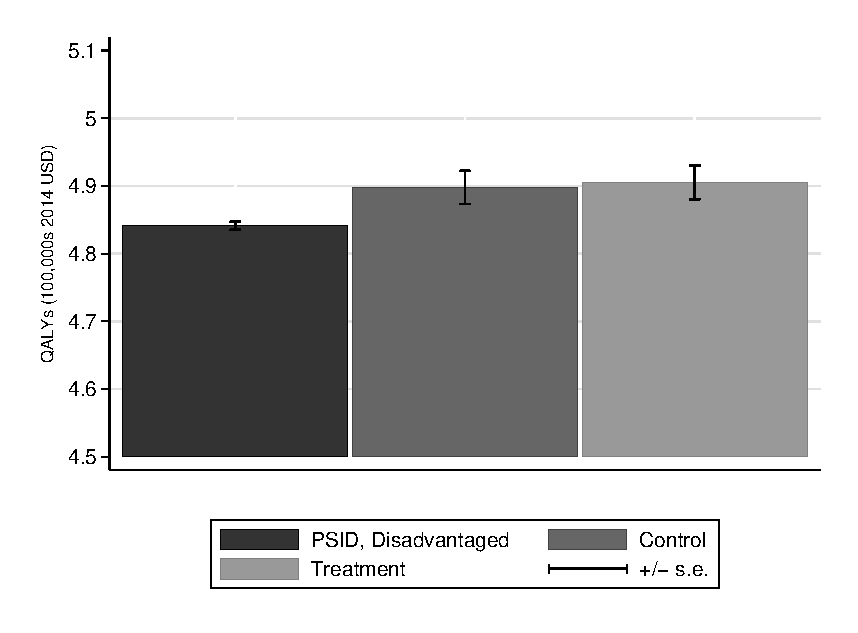
\includegraphics[width=\textwidth]{output/qalyexppsid_0.eps}
\end{subfigure}%
\begin{subfigure}[h]{0.5\textwidth}
	\centering
	\caption{Males} \label{fig:qpsid1}
		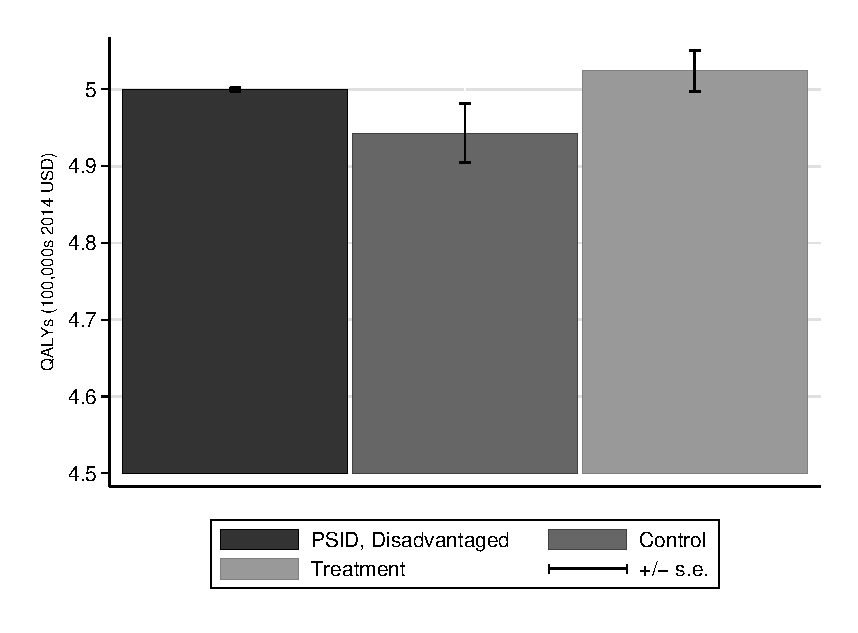
\includegraphics[width=\textwidth]{output/qalyexppsid_1.eps}
\end{subfigure}
\footnotesize \justify
Note: Panels (a) and (b) display the life-cycle net-present value of predicted quality-adjusted life years (QALYs) for ABC/CARE females and males, respectively, by treatment status. The predictions are based on combining data from the Panel Study of Income Dynamics (PSID), the Health Retirement Study, the Medical Expenditure Panel Survey (MEPS), and the Medicare Current Beneficiary Survey (MCBS). Each panel displays a comparison to to disadvantaged females and males in the Panel Study of Income Dynamics (PSID), where disadvantaged is defined as being black and having 12 years of education or less. QALYs are the quality-adjusted life years gain due to better health conditions. Standard errors are based on the empirical bootstrap distribution.\\
\end{sidewaysfigure}

\subsection{Crime}  \label{sec:crime}

To estimate the life-cycle benefits and costs of ABC/CARE related to criminal activity, we use rich data on crime outcomes obtained from public police records.\footnote{Two previous studies consider the impacts of ABC on crime: \citet{Clarke_Campbell_1998_ABC_Comparison_ECRQ} use administrative crime records up to age 21, and find no significant differences between the treatment and the control groups. \cite{Barnett_Masse_2002_benefitcost,Barnett_Masse_2007_EER} account for self-reported crime at age 21. They find little effects, but the lack longer term, administrative data.} See Appendix \ref{appendix:crime} for a more complete explanation of the following procedures. We consider the following types of crime: arson, assault, burglary, fraud, larceny, miscellaneous (which includes traffic and non-violent drug crimes), murder, vehicle theft, rape, robbery, and vandalism. We use administrative data that detail: (i) youth arrests, gathered at the age-21 follow-up; (ii) adult arrests, gathered at the age-34 follow-up; and (iii) sentences, gathered at the age-34 follow-up. We also use self-reported data on adult crimes, gathered in the age-21 and age-30 subject interviews. Because none of these sources capture all criminal activity, it is necessary to combine them to more completely approximate the crimes the subjects committed. We also use several auxiliary datasets to complete the life-cycle profile of criminal activity and compute the costs of the committed crimes

We follow four steps to estimate the costs of crime.

\begin{enumerate}
\item \textit{Count arrests and sentences.} We start by counting the total number of sentences for each individual and type of crime (arson, assault, etc.) up to age 34, matching crimes across data sources, to construct the total number of  arrests for each individual and type of crime up to age 34.\footnote{In practice, we count all offenses (an arrest might include multiple offenses). This gives the correct number of victims for our estimations. The youth data have coarser categories than the rest of the data: violent, property, drug, and other. To match these data with the adult data, we assume that all property crimes were larcenies and that all violent crimes are assaults. In the ABC/CARE sample, assault is the most common type of violent crime, and larceny/theft is the most common property crime.} For individuals missing arrest data,\footnote{About 10\% of the ABC/CARE sample has missing arrest data. We fail to reject differences in observed characteristics between the treatment- and control-group participants for whom we observe arrests data (see Appendix~\ref{appendix:data}).} we impute the number of arrests by multiplying the number of sentences for each type of crime by a national arrest-sentence ratio for the respective crime.\footnote{This arrest-sentence ratio is constructed using the National Crime Victimization Survey (NJRP) and the Uniform Crime Reporting Statistics (UCRS).}

\item \textit{Construct predictions.} Based on the sentences observed before age 34, we predict the sentences that the ABC/CARE subjects will have after age 34. Data from the North Carolina Department of Public Safety (NCDPS), which provide lifetime sentences of individuals in North Carolina, are used to estimate sentences incurred after age 34 from sentences incurred before age 34. Applying these models to the ABC/CARE data, we predict the number of future sentences for each subject up to age 50.\footnote{We assume that individuals with no criminal records before age 34 commit no crimes after age 34.} We then add these estimates to the original number of sentences, getting an estimate of the lifetime sentences. Adding these estimates increases the total count of crimes by 30\%--50\%.

\item \textit{Estimate number of victims from the crimes.} We only observe crimes that resulted in consequences in the justice system: crimes that resulted in arrests and/or sentences. To include unobserved crimes, we use victimization inflation (VI).\footnote{Previous papers using this method include \citet{Belfield_Nores_etal_2006_JHR} and \cite{Heckman_Moon_etal_2010_RateofReturn}.} We start by constructing a VI ratio, which is the national ratio of victims and arrests for each type of crime.\footnote{We assume that each crime with victims is counted separately in the national reports on arrests, even for arrests that might have been motivated by more than one crime. This victim-arrest ratio is constructed using the NJRP and the National Crime Victimization Survey (NCVS).} Then, we estimate the number of victims from the crimes committed by ABC/CARE subjects as their total arrests multiplied by the VI ratio.\footnote{Additionally, we can calculate an analogous estimate of the number of crime victims using sentences, based on the VI ratio and the national arrests-to-sentences ratio. Both estimates are very similar, as shown in Appendix \ref{appendix:crime}. To improve precision, the estimates in the rest of our paper are based on the average of the two calculations.}

\item \textit{Find total costs of crimes.} We use the estimates of the cost of crimes for victims from \cite{McCollister_etal_2010_DAD} to impute the total victimization costs. For crimes resulting in arrests and/or sentences, we consider justice system costs as well, such as police costs.\footnote{To be able to assign costs to each type of crime, we assume that the cost of the justice system depends on the number of offenses of each type, rather than on the number of arrests. While this could very slightly overestimate justice system costs, the costs only represent about 5\% of the total crime costs.} Finally, we construct the total costs of incarceration for each subject using the total prison time and the cost of a day in prison.\footnote{Appendix~\ref{appendix:sensitivity} examines the sensitivity of our crime costs quantification to different assumptions. Section~\ref{section:cbaresults} and Appendix~\ref{appendix:sensitivity} we examine the sensitivity of our overall assessment of ABC/CARE results to the quantification of crime that we explain in this section.}
\end{enumerate}

\subsection{Education}

Follow-up data on educational attainment were collected up to age 30. In Appendix \ref{appendix:education}, we show that using auxiliary data sources, education up to this age is an accurate predictor of lifetime educational attainment. Therefore, we do not predict beyond age 30. To monetize the costs of education, we consider the public costs of K-12 education and the private costs of post-secondary education, including vocational programs and community college. Other costs of education include grade retention and special education.

Previous analyses of ABC pay special attention to special education, arguing that savings due to a reduction in this category are substantial \citep{Barnett_Masse_2002_benefitcost,Barnett_Masse_2007_EER}.\footnote{This analyses does not include CARE.} This category is much less important in our calculation; pooling males and females the net gain due to a reduction in special education is $\$3,633.3$ (2014 USD) (s.e. $703.7)$.\footnote{This quantity is not discounted for comparability with other analyses. For males the gain is $\$13,417.9$ (2014 USD) (s.e. $1,061.0$) and for females there is actually a loss of $6,276.5$ (2014 USD) (s.e. $\$1,018.5$).}

\section{Benefit/Cost Analysis} \label{section:cbaresults}

This section reports cost/benefit and rate of return analyses underlying Figure~\ref{figure:main}. The results we discuss are the central focus of this paper. Appendix~\ref{appendix:sensitivity} displays an intensive sensitivity analysis of each of the components we consider in our main results. It includes scenarios in which all our assumptions hold and scenarios in which they are drastically violated, providing bounds for our estimates. It is an extension of the sensitivity analysis presented in Table~\ref{table:cba}.

\subsection{Program Costs} \label{section:programscosts}

The yearly cost of the program was \$18,514 per participant in 2014 USD. We improve on previous cost estimates using primary-source documents.\footnote{Our calculations are based on progress reports written by the principal investigators and related documentation recovered in the archives of the research center where the program was implemented. We display these sources in Appendix \ref{app:programcosts}. The main component is related to staff costs. Other costs arise from nutrition and services that the subjects received when they were sick, diapers during the first 15 months of their lives, and transportation to the center. The control-group children also received diapers during approximately 15 months, and iron-fortified formula. The costs are based on sources describing ABC treatment for $52$ children. We use the same costs estimates for CARE, for which information is less available. The costs exclude any expenses related to research or policy analysis. Our calculation of the costs per year in 1979 USD is $\$295,239$. A separate calculation of the program as implemented indicates that the yearly cost of the program was $\$275,475$ (1979 USD). See Appendix \ref{app:programcosts}.}

\subsection{Benefit/Cost Estimates}

\noindent \textbf{[JLG: I experimented with changing this section, but we can revert it back. The plots were too busy and are hard to read and grasp. The drastic sensitivity analysis seems also excessive as a first approach. I created tables that present the baseline estimates and depart from them in a more sensible way, I believe. We have all the previous material, so we can revert back.] [JJH: Typists, give me the old version as well as this so I can compare.] [Typist: This has been printed for you.]}

\begin{comment}
Figure~\ref{figure:npvs} presents the net present values for the main components of the cost/benefit analysis pooling males and females. The ``Treatment vs. Next Best'' bars represent the estimates based on the first parameter of interest, comparing the treatment- to the control-group subjects. The ``Treatment vs.  Stay at Home'' bars represent the comparison between the treatment-group and the control-group subjects who stayed at home. The ``Treatment vs. Alternative Preschool'' bars represent the comparison between the treatment-group and the control-group subjects who attended alternative preschools.

The first category, ``Program Costs," represents the cost of the programs' implementation. The second category, ``Total Net Benefits" quantifies the benefits for the treatment-group subjects net of the benefits of the control-group subjects. We consider labor income of both the participants and of their parents, ``Labor Income" and ``Parental Income." The program produces a positive net present value on labor income of the treated subjects. This considers income from age 21 all the way to retirement.

Crime is an important component of the benefit/cost ratios, which is consistent with previous analysis of early childhood education programs.\footnote{\citet{Heckman_Moon_etal_2010_RateofReturn}.} We then present two main categories for health, ``QALYs" and ``Medical Costs." As documented in \citet{Campbell_Conti_etal_2014_EarlyChildhoodInvestments}, ABC/CARE had substantial effects on several measures of long-term health, especially for males---e.g. body-mass index, systolic and diastolic pressure, Framigham risk index. This translates into a higher probability of survival at later ages. Thus, individuals in the treatment group incur higher medical costs. However, their health conditions enable them to have higher quality lives, which is reflected in the net gain the program generates in the QALYs. Finally, we present the net present value of education costs. It is negative because subjects in the treatment group acquired more education throughout their life cycles.

It is important to note that although the net present values from the three comparisons imply that ABC/CARE is socially beneficial regardless of control substitution, the magnitudes for some of the components vary substantially. We argue that this has to do with the differential treatment effects of ABC/CARE by gender. As Figure~\ref{figure:npvsf} and Figure~\ref{figure:npvsm} show, males benefit much more when the counterfactual scenario attending an alternative preschool, while females benefit much more from the program when the counterfactual scenario is to staying at home.

\begin{sidewaysfigure}[!htbp]
\caption{Life-cycle Net Present Value of Main Components of the CBA, Pooled Sample of Males and Females}
\label{figure:npvs}
\centering
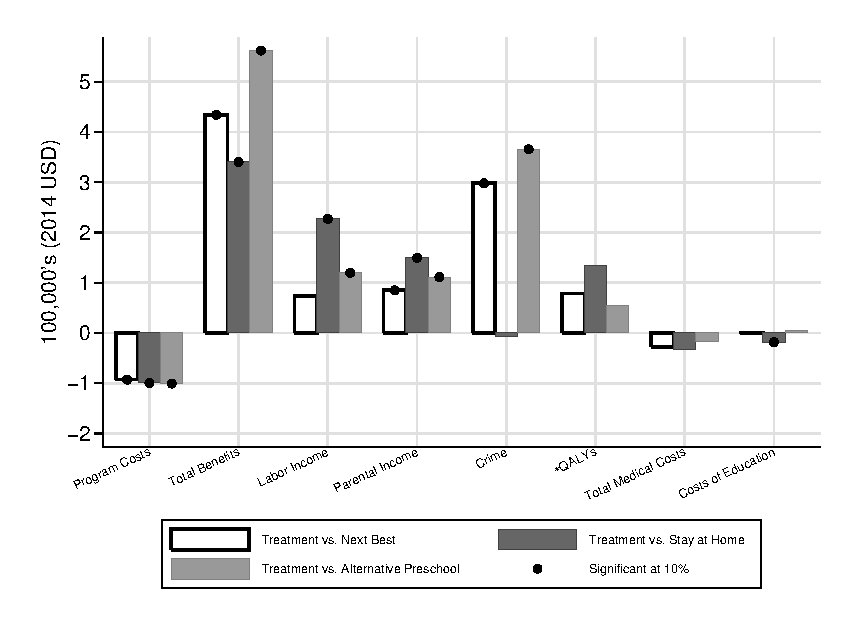
\includegraphics[width=.7\columnwidth]{output/abccare_npvs3.eps}
\floatfoot{
\footnotesize
Note: This figure displays the life-cycle net present values of the main components of the cost/benefit analysis of ABC/CARE from birth to age 79, discounted to birth at a rate of 3\%. ``Treatment vs. Control'': compares the treatment to the control group. ``Treatment vs. Stay at Home'': compares the treatment group to those subjects who stayed at home. ``Treatment vs. Alternative Preschool'': compares the treatment group to those subjects who attended alternative preschools. The latter two are based on matching estimators that account for selection on observable variables. By ``net" we mean that each component represents the total value for the treatment group minus the total value for the control group. Program costs: the total cost of implementing ABC/CARE. Total net benefits: the total net benefits of \textit{all} the components we consider. Labor income: total individual labor income from ages 20 to the retirement of program participants  (assumed to be age 67). Parental income: total parental labor income of the parents of the program participants from when the participants were ages 1.5 to 21. Crime: the total cost of crime (judicial and victimization costs). Total medical costs: both private and public medical costs from ages 15 to 79. Costs of education: the total costs of education of the individual from ages 6 to 26 and include any costs from special education and grade retention. For display simplicity, the following components are omitted from the figure: (i) cost of alternative preschool paid by the control group children parents; (ii) transfer income from the government; (iii) disability benefits and social security claims; and (iv) costs of increased maternal education. Inference is based on non-parametric, one-sided $p$-values from the empirical bootstrap distribution. We highlight point estimates significant at the $10\%$ level.\\
*QALYs refers to the quality-adjusted life years. Any gain corresponds to better health conditions through age 79.\\
}
\end{sidewaysfigure}

\begin{sidewaysfigure}[!htbp]
\caption{Life-cycle Net Present Value of Main Components of the CBA, Females}
\label{figure:npvsf}
\centering
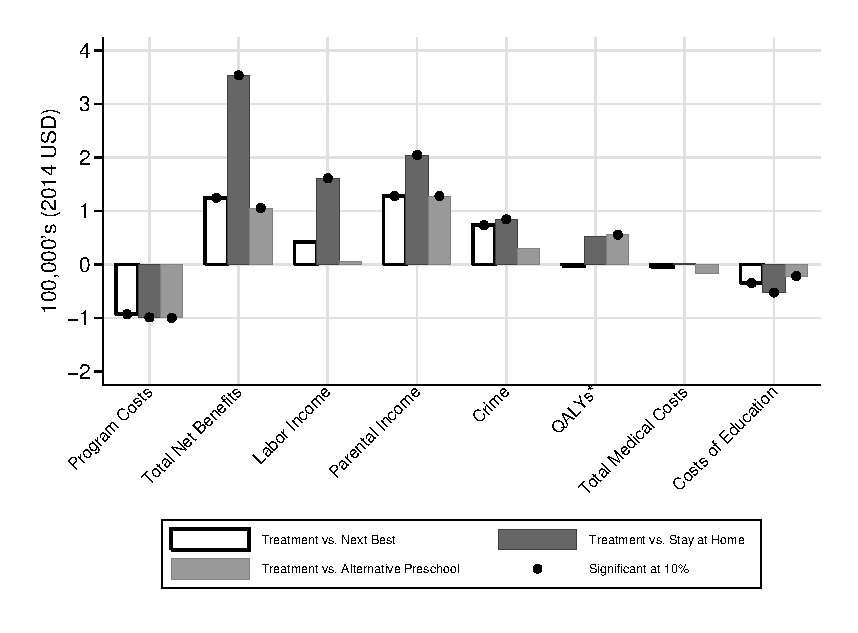
\includegraphics[width=.7\columnwidth]{output/abccare_npvs1.eps}
\floatfoot{
\footnotesize
Note: This figure displays the life-cycle net present values of the main components of the cost/benefit analysis of ABC/CARE from birth to age 79, discounted to birth at a rate of 3\%. ``Treatment vs. Control'': compares the treatment to the control group. ``Treatment vs. Stay at Home'': compares the treatment group to those subjects who stayed at home. ``Treatment vs. Alternative Preschool'': compares the treatment group to those subjects who attended alternative preschools. The latter two are based on matching estimators that account for selection on observable variables. By ``net" we mean that each component represents the total value for the treatment group minus the total value for the control group. Program costs: the total cost of implementing ABC/CARE. Total net benefits: the total net benefits of \textit{all} the components we consider. Labor income: total individual labor income from ages 20 to the retirement of program participants  (assumed to be age 67). Parental income: total parental labor income of the parents of the program participants from when the participants were ages 1.5 to 21. Crime: the total cost of crime (judicial and victimization costs). Total medical costs: both private and public medical costs from ages 15 to 79. Costs of education: the total costs of education of the individual from ages 6 to 26 and include any costs from special education and grade retention. For display simplicity, the following components are omitted from the figure: (i) cost of alternative preschool paid by the control group children parents; (ii) transfer income from the government; (iii) disability benefits and social security claims; and (iv) costs of increased maternal education. Inference is based on non-parametric, one-sided $p$-values from the empirical bootstrap distribution. We highlight point estimates significant at the $10\%$ level.\\
*QALYs refers to the quality-adjusted life years. Any gain corresponds to better health conditions through age 79.\\
}
\end{sidewaysfigure}

\begin{sidewaysfigure}[!htbp]
\caption{Life-cycle Net Present Value of Main Components of the CBA, Males}
\label{figure:npvsm}
\centering
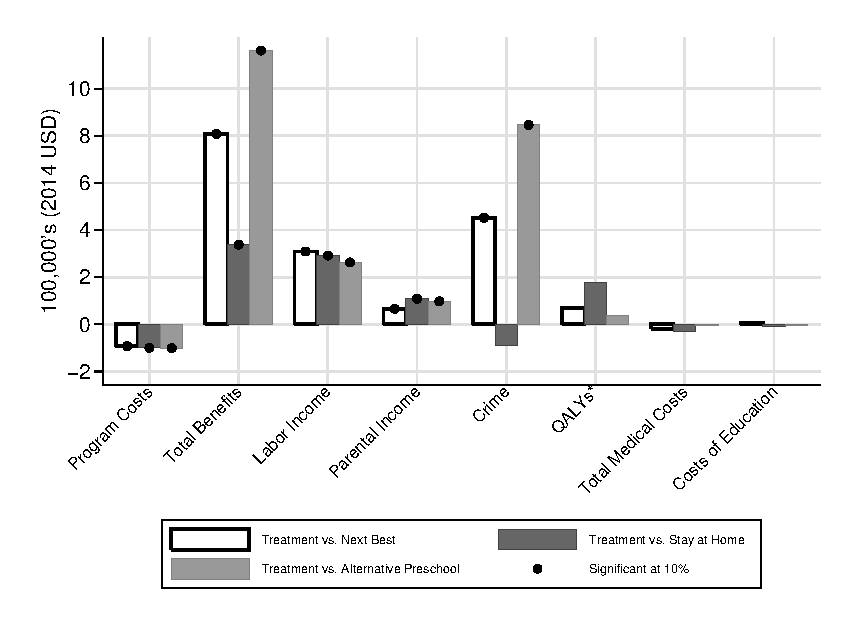
\includegraphics[width=.7\columnwidth]{output/abccare_npvs2.eps}
\floatfoot{
\footnotesize
Note: This figure displays the life-cycle net present values of the main components of the cost/benefit analysis of ABC/CARE from birth to age 79, discounted to birth at a rate of 3\%. ``Treatment vs. Control'': compares the treatment to the control group. ``Treatment vs. Stay at Home'': compares the treatment group to those subjects who stayed at home. ``Treatment vs. Alternative Preschool'': compares the treatment group to those subjects who attended alternative preschools. The latter two are based on matching estimators that account for selection on observable variables. By ``net" we mean that each component represents the total value for the treatment group minus the total value for the control group. Program costs: the total cost of implementing ABC/CARE. Total net benefits: the total net benefits of \textit{all} the components we consider. Labor income: total individual labor income from ages 20 to the retirement of program participants  (assumed to be age 67). Parental income: total parental labor income of the parents of the program participants from when the participants were ages 1.5 to 21. Crime: the total cost of crime (judicial and victimization costs). Total medical costs: both private and public medical costs from ages 15 to 79. Costs of education: the total costs of education of the individual from ages 6 to 26 and include any costs from special education and grade retention. For display simplicity, the following components are omitted from the figure: (i) cost of alternative preschool paid by the control group children parents; (ii) transfer income from the government; (iii) disability benefits and social security claims; and (iv) costs of increased maternal education. Inference is based on non-parametric, one-sided $p$-values from the empirical bootstrap distribution. We highlight point estimates significant at the $10\%$ level.\\
*The treatment vs. stay at home net present value is sizable and negative (-\$91,476.3); its standard error is 86,657.3.\\
**QALYs refers to the quality-adjusted life years. Any gain corresponds to better health conditions through age 79.\\
}
\end{sidewaysfigure}

We compute the internal rate of return and benefit/cost ratio implied by the net present values presented in Figure~\ref{figure:npvs} through Figure~\ref{figure:npvsm}. The results without accounting for control substitution are presented in Table~\ref{table:cba}. All the monetary figures are in 2014 USD and are discounted to each child's birth, at a $3\%$ discount rate.\footnote{We present sensitivity analysis to different discount rates in Table~\ref{table:cba} and in Appendix~\ref{appendix:sensitivity}.}

\end{comment}

Table~\ref{table:bcsens} presents our baseline estimates of benefit/cost ratios, Table~\ref{table:irrsens} presents the analogous internal rates of return. Pooling males and females, the results indicate that the program is socially efficient: the internal rate of return and the benefit/cost ratio are $12.6\%$ and $5.6$. \textit{The program generates a benefit of \bcp\ for every dollar spent on it}. They are statistically significant, even after accounting for sampling variation, serial correlation, and forecasting error in the experimental and non-experimental samples and the tax costs of financing the program. These results are important because ABC/CARE was much more expensive than other early childhood education programs---the treatment involved more services over a longer time period \citep{Elango_Hojman_etal_2016_Early-Edu}.

We accompany these estimates with a set of sensitivity checks of statistical and economic interest. Our estimates are not driven by our methods for accounting for attrition and item non-response or by the conditioing variables we used when computing the net-present values (specification columns).  Although the internal rate of return remains relatively high when using participant outcome measures up to ages 21 or 30, the benefit/cost ratios indicate that accounting for benefits that go beyond age 30 is relevant. The return to each dollar is at most $3/1$ when considering benefits up to age 30 only (prediction span columns). The counterfactuals considered also make a difference. Males benefit the most from ABC/CARE relative to alternative preschools, while females benefit the most from ABC/CARE relative to staying at home. We further explore this difference below.

Our baseline estimates account for the deadweight caused by the government by taxing individuals to budget its expenditure for all government-related activities.\footnote{When the transaction between the government and an individual is a direct transfer, we consider .5 as a cost per each transacted dollar as we do not weight the final recipient of the transaction (e.g., transfer income). When the transaction is indirect, we classify it as government spending as a whole and consider its cost as 1.5 per each dollar spend (e.g. public education).} Our baseline estimate assumes that the marginal tax rate is $50\%$. Our estimates are robust to dropping it to $0\%$ or doubling it to $100\%$ (deadweight loss columns). Our baseline estimation of benefit/cost ratios is based on a discount rate of $3\%$. Not discounting roughly doubles our benefit/cost ratios, while they remain significant under a higher discount rate of $7\%$ (discount rate columns).

Parental income is an important component of the benefit/cost ration. As explained in Section~\ref{section:pincome}, we take a conservative approach in our baseline estimates and do not account for the potential profile shift in parental income due to education and experience. This is based on observed parental income from when the ABC/CARE participants where ages 0 to 21. Alternative approaches considering the gain up to when the parent is 65 years old generate an increase in the gain due to parental income (parental income columns). As we mention in Section~\ref{section:cbamethodology}, our estimates ignore any cohort effects. Individuals in ABC/CARE could experience positive cohort effects that might (i) make them more productive and therefore experience wage growth \citep{Lagakos_Moll_etal_2016_LifeCycle_NBER}; (ii) experience a negative shock such as an economic crisis and therefore experience wage decline \citep{Jarosch_2016_JobSecurity_Econometrica}. Our estimates are robust when we vary annual growth and decay rates between $-.5\%$ to $.5\%$.

We do not perform sensitivity analysis to investigate cohort effects of health costs. Treatment individuals are healthier, which reduces medical costs, but also that they live longer, increasing medical costs. These opposing effects negate each other. We have little guidance for forecasting the future health costs and benefits of our cohort compared to the cohorts on which FAM is based.

\newgeometry{top=.6in, bottom=.6in, left=.6in, right=.6in}
\begin{sidewaystable}[!htpb]
\begin{threeparttable}
\caption{Sensitivity Analysis for Benefit/Cost Ratios}
\label{table:bcsens}
\centering
\footnotesize
\begin{tabular}{>{\bfseries}lcc|cc|cc} \toprule
	&	\multicolumn{2}{c}{\textbf{\textit{Pooled}}}	&	\multicolumn{2}{c}{\textbf{\textit{Males}}}	&	\multicolumn{2}{c}{\textbf{\textit{Females}}}	\\ 
Baseline	&	\multicolumn{2}{c}{5.69 (s.e. 2.32)}	&	\multicolumn{2}{c}{11.62 (s.e. 5.49)}	&	\multicolumn{2}{c}{2.60 (s.e. 0.98)}	\\ \\
\multicolumn{7}{l}{\textit{Baseline: IPW and Controls, Life-span up to Age 79, Treatment vs. Next Best, 50\% Marginal tax 50\% (deadweight loss), Discount rate 3\%, Parental}} \\	
\multicolumn{7}{l}{\textit{income 0 to 21 (child's age), Labor Income predicted from 21 to 65, All crimes (full costs), Value of life 150,000.}} \\ \\ \midrule	
Specification	&	\textit{No IPW}	&	\textit{and No Controls}	&	\textit{No IPW}	&	\textit{and No Controls}	&	\textit{No IPW}	&	\textit{and No Controls}	\\
	&	\textbf{6.17}	&	\textbf{5.35}	&	\textbf{11.94} 	&	\textbf{10.74}	&	\textbf{2.91}	&	\textbf{2.79}	\\
	&	(2.35)	&	(2.04)	&	(6.14)	&	(4.12)	&	(0.97)	&	(0.81)	\\ \midrule
Prediction	&	\textit{to Age 21}	&	\textit{to Age 30}	&	\textit{to Age 21}	&	\textit{to Age 30}	&	\textit{to Age 21}	&	\textit{to Age 30}	\\
Span	&	\textbf{1.55}	&	2.01	&	\textbf{2.17}	&	2.80	&	1.17	&	1.52	\\
	&	(0.39)	&	(0.88)	&	(0.74)	&	(1.96)	&	(0.43)	&	(0.48)	\\ \midrule
Counter-	&	\textit{vs. Stay at Home}	&	\textit{vs. Alt. Presch.}	&	\textit{vs. Stay at Home}	&	\textit{vs. Alt. Presch.}	&	\textit{vs. Stay at Home}	&	\textit{vs. Alt. Presch.}	\\
factuals	&	\textbf{4.44}	&	\textbf{6.58}	&	3.88	&	\textbf{10.85}	&	\textbf{4.89}	&	\textbf{2.40}	\\
	&	(1.68)	&	(2.22)	&	(2.78)	&	(4.14)	&	(1.50)	&	(0.94)	\\ \midrule
Deadweight-	&	\textit{0\%}	&	\textit{100\%\textit}	&	\textit{0\%}	&	\textit{100\%\textit}	&	\textit{0\%}	&	\textit{100\%\textit}	\\
loss	&	\textbf{8.50}	&	\textbf{4.29}	&	\textbf{17.43}	&	\textbf{8.71}	&	\textbf{3.69}	&	2.06	\\
	&	(3.47)	&	(1.75)	&	(8.19)	&	(4.14)	&	(1.43)	&	(0.79)	\\ \midrule
Discount 	&	\textit{0\%}	&	\textit{7\%}	&	\textit{0\%}	&	\textit{7\%}	&	\textit{0\%}	&	\textit{7\%}	\\
Rate	&	13.38	&	2.40	&	29.50	&	4.21	&	5.34	&	1.43	\\
	&	7.01	&	0.80	&	15.93	&	1.88	&	3.81	&	0.37	\\ \midrule
Parental	&	\textit{Mincer Life-cycle}	&	\textit{Life-cycle Prediction}	&	\textit{Mincer Life-cycle}	&	\textit{Life-cycle Prediction}	&	\textit{Mincer Life-cycle}	&	\textit{Life-cycle Prediction}	\\
Income	&	\textbf{5.92}	&	\textbf{5.60}	&	\textbf{11.80}	&	\textbf{12.36}	&	\textbf{2.88}	&	\textbf{3.27}	\\
	&	(2.32)	&	(2.39)	&	(5.49)	&	(5.68)	&	(1.02)	&	(1.21)	\\ \midrule
Labor	&	\textit{.5\% Annual Decay}	&	\textit{.5\% Annual Growth}	&	\textit{.5\% Annual Decay}	&	\textit{.5\% Annual Growth}	&	\textit{.5\% Annual Decay}	&	\textit{.5\% Annual Growth}	\\
Income	&	\textbf{5.48}	&	\textbf{5.90}	&	\textbf{10.76}	&	\textbf{12.49}	&	\textbf{2.47}	&	\textbf{2.74}	\\
	&	(2.25)	&	(2.41)	&	(5.33)	&	(5.71)	&	(0.87)	&	(1.10)	\\ \midrule
Crime	&	\textit{Drop Major Crimes}	&	\textit{Halve Costs}	&	\textit{Drop Major Crimes}	&	\textit{Halve Costs}	&	\textit{Drop Major Crimes}	&	\textit{Halve Costs}	\\
	&	\textbf{5.14} 	&	\textbf{4.07}	&	\textbf{11.82}	&	\textbf{8.33}	&	\textbf{2.72}	&	2.25	\\
	&	(2.30)	&	(1.50)	&	(5.59)	&	(3.64)	&	(1.04)	&	(0.95)	\\ \midrule
Health	&	\textit{Drop All}	&	\textit{Double Value of Life}	&	\textit{Drop All}	&	\textit{Double Value of Life}	&	\textit{Drop All}	&	\textit{Double Value of Life}	\\
(QALYs)	&	\textbf{4.85}	&	\textbf{6.56}	&	\textbf{10.61}	&	\textbf{12.63}	&	\textbf{2.48}	&	2.73	\\
	&	(2.32)	&	(2.54)	&	(5.37)	&	(5.90)	&	(0.97)	&	(1.26)	\\ \bottomrule
\end{tabular} 
\begin{tablenotes}
\footnotesize
\item Note: This table displays sensitivity analysis of our baseline benefit/cost ratio calculation to the perturbations indexed in the different rows. The characteristics of the \textit{baseline} calculation are in the table header. IPW: adjusts for attrition and item non-response (see Appendix~\ref{appendix:attrition} for details). Controls: Apgar scores at ages 1 and 5 and a high-risk index (see Appendix~\ref{appendix:results} for details on how we choose these controls). When predicting up to ages 21 and 30, we consider all benefits and costs up to these ages, respectively. Counterfactuals: we consider treatment vs. next best (baseline), treatment vs. stay at home, and treatment vs. alternative preschools (see Section~\ref{section:methodsquestions} for a discussion). Deadweight loss is the loss implied by any public expenditure (0\% is no loss and 100\% is one dollar loss per each dollar spent). Discount rate: rate to discount benefits to child's age 0 (in all calculations). Parental income: see Appendix~\ref{app:parentalincome} for details on the two alternative predictions (Mincer and Life-cycle). Labor Income: .5\ annual growth (decay) is an annual wage growth (decay) due to cohort effects. Crime: major crimes are rape and murder; half costs takes half of victimization and judiciary costs. Health (QALYs): drop all sets the value of life equal to zero. Standard errors obtained from the empirical bootstrap distribution are in parentheses. Bolded $p$-values are significant at 10\%. For details on the null hypothesis see Table~\ref{table:cba}.
\end{tablenotes}
\end{threeparttable}
\end{sidewaystable}

\begin{sidewaystable}[!htpb]
\begin{threeparttable}
\caption{Sensitivity Analysis for Internal Rate of Return, ABC/CARE}
\label{table:irrsens}
\centering
\footnotesize
% matrix: allirr file: allirr_sens.tex  25 Sep 2016 09:11:16
\begin{table}[htbp]
\begin{tabular}{lcccccc} \hline \hline
 & pooled  & pooled  & males  & males  & females  & females  \\  \hline 
baseline &     0.087 &     0.052 &     0.138 &     0.048 &     0.126 &     0.048 \\  
specification &     0.092 &     0.087 &     0.147 &     0.148 &     0.136 &     0.122 \\  
. &     0.059 &     0.032 &     0.060 &     0.037 &     0.044 &     0.039 \\  
predictiontime &     0.099 &     0.127 &     0.110 &     0.127 &     0.104 &     0.115 \\  
. &     0.056 &     0.051 &     0.047 &     0.051 &     0.045 &     0.043 \\  
counterfactual &     0.131 &     0.089 &     0.085 &     0.162 &     0.100 &     0.132 \\  
. &     0.046 &     0.057 &     0.038 &     0.044 &     0.034 &     0.039 \\  
dwl &     0.128 &     0.068 &     0.175 &     0.118 &     0.174 &     0.103 \\  
. &     0.089 &     0.037 &     0.063 &     0.042 &     0.064 &     0.037 \\  
parental &     0.104 &         . &     0.148 &         . &     0.142 &         . \\  
. &     0.069 &         . &     0.053 &         . &     0.053 &         . \\  
lincome &     0.080 &         . &     0.127 &         . &     0.122 &         . \\  
. &     0.053 &         . &     0.054 &         . &     0.047 &         . \\  
crime &     0.089 &     0.081 &     0.153 &     0.122 &     0.124 &     0.110 \\  
. &     0.052 &     0.051 &     0.043 &     0.046 &     0.044 &     0.044 \\  
health &     0.091 &     0.085 &     0.136 &     0.134 &     0.112 &     0.127 \\  
. &     0.053 &     0.052 &     0.049 &     0.053 &     0.058 &     0.045 \\  
\hline \hline \end{tabular}
\end{table}

\begin{tablenotes}
\footnotesize
\item Note: This table displays sensitivity analysis of our baseline internal rate of return calculation to the perturbations indexed in the different rows. The characteristics of the \textit{baseline} calculation are in the table header. IPW: adjusts for attrition and item non-response (see Appendix~\ref{appendix:attrition} for details). Controls: Apgar scores at ages 1 and 5 and a high-risk index (see Appendix~\ref{appendix:results} for details on how we choose these controls). When predicting up to ages 21 and 30, we consider all benefits and costs up to these ages, respectively. Counterfactuals: we consider treatment vs. next best (baseline), treatment vs. stay at home, and treatment vs. alternative preschools (see Section~\ref{section:methodsquestions} for a discussion). Deadweight loss is the loss implied by any public expenditure (0\% is no loss and 100\% is one dollar loss per each dollar spent). Parental income: see Appendix~\ref{app:parentalincome} for details on the two alternative predictions (Mincer and Life-cycle). Labor Income: .5\ annual growth is an annual wage growth due to cohort effects; only benefit assumes labor income is the only benefit of the program. Crime: major crimes are rape and murder; half costs takes half of victimization and judiciary costs. Health (QALYs): drop all sets the value of life equal to zero. N/A: Standard errors obtained from the empirical bootstrap distribution are in parentheses. Bolded $p$-values are significant at 10\%. For details on the null hypothesis see Table~\ref{table:cba}.
\end{tablenotes}
\end{threeparttable}
\end{sidewaystable}
\restoregeometry
\doublespacing

We also examine the sensitivity to (i) dropping the most costly crimes as murders and rapes;\footnote{Two individuals in the treatment group committed a rape and one individual in the control group committed a murder.} and (ii) halving the costs of victimization and judiciary costs related to crime.  The first is important because we would not want our calculation to be based on a few exceptional crimes. The second is important because victimization costs are somewhat subjective (see Appendix~\ref{appendix:crime}). Our benefit/cost analysis is robust to these adjustments, even when crime is a major component. Lastly, we examine the sensitivity with respect to our main health component: quality-adjusted life years. This is an important component because relatively healthier individuals survive longer and healthier, and treatment improves health conditions. However, it is important to note that this component largely accumulates later in life and therefore it is heavily discounted. Dropping the component or doubling the value of life does not have a major impact in our calculations.

The estimates are robust when we conduct a drastic sensitivity analysis by removing components of the benefit/cost analysis entirely (Table~\ref{table:cba}).\footnote{In Appendix~\ref{appendix:sensitivity}, we present exercises that are not as drastic as removing the whole component, but instead removing fractions of it.} Even when completely removing the gain associated with crime for males, the program is socially efficient. Both the internal rate of return and the benefit/cost ratio are substantial. Parental income and crime are the components for which the internal rate of return and the benefit/cost ratio are the most sensitive. The reason for the sensitivity to parental income is that the amount is substantial and it is not heavily discounted because it accumulates during the first $21$ years of the children's life. Crime occurs later in life and its benefits are discounted accordingly. The amount due to crime savings is large so removing it diminishes both the internal rate of return and the benefit/cost ratio (but they remain statistically significant).

\begin{table}[!htbp]
\centering
\caption{Cost/benefit Analysis of ABC/CARE, Summary}\label{table:cba}
\begin{adjustbox}{max width=\textwidth}
\begin{threeparttable}
\begin{tabular}{l r r r r r r r r r}																			
\toprule																			
&       \mc{3}{c}{Females}      &       \mc{3}{c}{Males}        &       \mc{3}{c}{Pooled}       \\																			
\cmidrule(lr){2-4}      \cmidrule(lr){5-7}      \cmidrule(lr){8-10}																			
Removed Component       &       NPV     &       IRR     &       B/C     &       NPV     &       IRR     &       B/C     &       NPV     &       IRR     &       B/C     \\																			
\midrule																			
None	&	161,759	&	\textbf{10.1\%}	&	\textbf{2.61}	&	919,049	&	\textbf{14.7\%}	&	\textbf{10.19}	&	636,674	&	\textbf{13.7\%}	&	\textbf{7.33}	\\
	&		&	(6\%)	&	(0.73)	&		&	(4\%)	&	(2.93)	&		&	(3\%)	&	(1.84)	\\ \\
Parental Income	&	148,854	&	4\%	&	1.12	&	107,907	&	\textbf{11\%}	&	\textbf{9.10}	&	116,953	&	\textbf{9\%}	&	\textbf{6.17}	\\
	&		&	(2\%)	&	(0.65)	&		&	(3\%)	&	(2.92)	&		&	(3\%)	&	(1.87)	\\
Subject Labor Income	&	41,908	&	9\%	&	\textbf{2.21}	&	238,105	&	\textbf{13\%}	&	\textbf{7.75}	&	133,032	&	\textbf{13\%}	&	\textbf{6.03}	\\
	&		&	(6\%)	&	(0.66)	&		&	(5\%)	&	(2.23)	&		&	(4\%)	&	(1.77)	\\
Subject Transfer Income	&	419	&	\textbf{10\%}	&	\textbf{2.61}	&	-7,265	&	\textbf{15\%}	&	\textbf{10.26}	&	-4,372	&	\textbf{14\%}	&	\textbf{7.38}	\\
	&		&	(6\%)	&	(0.73)	&		&	(4\%)	&	(2.93)	&		&	(3\%)	&	(1.84)	\\
Subject QALY	&	42,102	&	9\%	&	\textbf{2.20}	&	106,218	&	\textbf{14\%}	&	\textbf{9.14}	&	87,181	&	\textbf{13\%}	&	\textbf{6.48}	\\
	&		&	(6\%)	&	(0.69)	&		&	(6\%)	&	(2.73)	&		&	(5\%)	&	(1.79)	\\
Medical Expenditures	&	-16,037	&	9\%	&	\textbf{2.77}	&	-42,038	&	\textbf{15\%}	&	\textbf{10.61}	&	-31,221	&	\textbf{14\%}	&	\textbf{7.65}	\\
	&		&	(6\%)	&	(0.76)	&		&	(3\%)	&	(2.89)	&		&	(3\%)	&	(1.85)	\\
Alternative Preschools	&	16,691	&	8\%	&	\textbf{2.45}	&	13,434	&	\textbf{14\%}	&	\textbf{10.05}	&	14,659	&	\textbf{12\%}	&	\textbf{7.19}	\\
	&		&	(5\%)	&	(0.73)	&		&	(4\%)	&	(2.92)	&		&	(3\%)	&	(1.84)	\\
Education Costs	&	1,457	&	\textbf{10\%}	&	\textbf{2.59}	&	-7,852	&	\textbf{15\%}	&	\textbf{10.26}	&	-4,518	&	\textbf{14\%}	&	\textbf{7.37}	\\
	&		&	(6\%)	&	(0.72)	&		&	(4\%)	&	(2.93)	&		&	(3\%)	&	(1.86)	\\
Crime Costs	&	31,668	&	10\%	&	\textbf{2.34}	&	638,923	&	\textbf{9\%}	&	4.08	&	450,368	&	\textbf{8\%}	&	\textbf{3.06}	\\
	&		&	(6\%)	&	(0.62)	&		&	(5\%)	&	(2.18)	&	&	(4\%)	&	(1.01)	\\ \\
Deadweight Loss	&		&	\textbf{18\%}	&	\textbf{3.83}	&		&	\textbf{19\%}	&	\textbf{15.38}	&		&	\textbf{18\%}	&	\textbf{11.01}	\\
	&		&	(12\%)	&	(1.04)	&		&	(6\%)	&	(4.35)	&		&	(5\%)	&	(2.79)	\\
0\% Discount Rate	&		&		&	\textbf{5.06}	&		&		&	\textbf{25.45}	&		&		&	\textbf{17.40}	\\
	&		&		&	(2.82)	&		&		&	(10.42)	&		&		&	(5.90)	\\
7\% Discount Rate	&		&		&	\textbf{1.49}	&		&		&	\textbf{3.78}	&		&		&	\textbf{2.91}	\\
	&		&		&	(0.32)	&		&		&	(0.79)	&		&		&	(0.59)	\\
\bottomrule																			
\end{tabular}																			

\begin{tablenotes}
\footnotesize
\item Note: This table presents the estimates of the net present value (NPV) for each component, and the internal rate of return (IRR) and the benefit/cost ratio (B/C) of ABC/CARE for different scenarios based on comparing the groups randomly assigned to receive center-based childcare and the groups randomly assigned as control in ABC/CARE. The first row represents the baseline estimates. The rest of the rows present estimates for scenarios in which we remove the NPV estimates of the component listed in the first column. Alternative Preschools refer to money spent in alternatives to treatment from the control-group children parents. QALYs refers to the quality-adjusted life years. Any gain corresponds to better health conditions through age 79. The quantity listed in the NPV columns is the component we actually remove when computing the calculation in each row. All the money figures are in 2014 USD and are discounted to each child's birth, unless otherwise specified. For the B/C we use a discount rate of $3\%$, unless otherwise specified. We test the null hypotheses $\text{IRR} = 3\%$ and $\text{B/C} = 1$---we elect $3\%$ because that is the discount rate we use. Inference is based on non-parametric, one-sided $p$-values from the empirical bootstrap distribution. We highlight point estimates significant at the $10\%$ level.\\
\textit{Total cost of the program per child is $92,570$.}
\end{tablenotes}
\end{threeparttable}
\end{adjustbox}
\end{table}

\subsection{Possible Explanations for Gender Differences}

The benefit/cost ratio and internal rate of return calculations both indicate that males and females benefit \emph{differently} from the program. There are two complementary stories to reconcile this difference. First, we explore reasons why the differences could exists if we focus on the outcomes we are monetizing, and not on the counterfactual we are studying. Males have relatively high benefits from outcomes that we are able to monetize: labor income and crime are two examples of this. Historically, females are less likely to supply labor than males \citep{Jaumotte_2003_OECD}. While all males supply labor in our sample at age 30, not all females supply labor. We are not able to quantify household production benefits to the treated males and females. This is an important omission for females who decide to stay at home instead of working.\footnote{The issue of females labor supply being fundamentally different from males labor supply has been noted in the Economics literature for a long time and it has posed methodological challenges (see \citet{Killingsworth_Heckman_1986_FemaleLaborSupply} for a first survey of the issues in modern Econometrics). Not being able to monetize household production is a well-known and discussed issue as well \citep{Becker_1995_Housework_Bloomberg}.}

Evidence shows, also, that males are much more likely to commit crimes that are more costly to the victims and to the judiciary system \citep{Cohen-Bowles_2010_Estimating-Cost-Crime,Gregg_etal_2015_SocialRealities_BOOK}. It s not the case that ABC/CARE does not have treatment effects on crime for females. Actually, there are effects on a number of categories (see Appendix~\ref{appendix:results}). However, males commit crimes that are much more expensive. These two categories are examples of why the magnitudes of the gains are much higher for males than they are for females.

For health, the gender differences are substantial as well. But both males and females have substantial gains: males on more standard measures of physical health, while females on a set of mental health measures (see Appendix~\ref{appendix:results}). We quantify both of these components (see Section~\ref{section:health} and Appendix~\ref{appendix:health}).

When analyzing different counterfactuals, there is a substantial difference between males and females. The difference is driven by one of the counterfactuals: treatment vs. alternative preschools. The estimates for both males and females generate a similar assessment of ABC/CARE treatment if compared to stay at home. It is the case that males benefit much more than treatment relative to alternative preschools than what they benefit of treatment relative to staying at home. This result is consistent three sets of findings noted elsewhere: (i) stark gender differences resulting from attending childcare\citep{Kottelenberg-Lehrer_2014_Gender-Effects,Baker_Gruber_Milligan_2015_Noncog_Defects,Doyle-etal_2015_Econ-Hum-Bio,Doyle-etal_2016_PLoS-ONE}; (ii) females being less sensitive to uncertain environments \citep{Autor-etal_2015_Family-Disadvantage} and (iii) maternal absence being more deleterious for males \citep{Rutter_1972_Maternal-Deprivation}.

The evidence we show does not indicate that the program has no benefit for females; in fact it does. If compared to staying at home, the gain for females indicates that there is a gain of $4.81$ dollars per each dollar invested. In fact, when we decompose the net-present value for each of the components that we monetize, we see substantial benefits for females across various categories. Health and crime included. For males, the magnitudes are noticeably reinforce when comparing treatment to alternative preschool (see Figures ~\ref{figure:npvsf} and \ref{figure:npvsm}).

\begin{sidewaysfigure}[!htbp]
\caption{Life-cycle Net Present Value of Main Components of the CBA, Females}
\label{figure:npvsf}
\centering
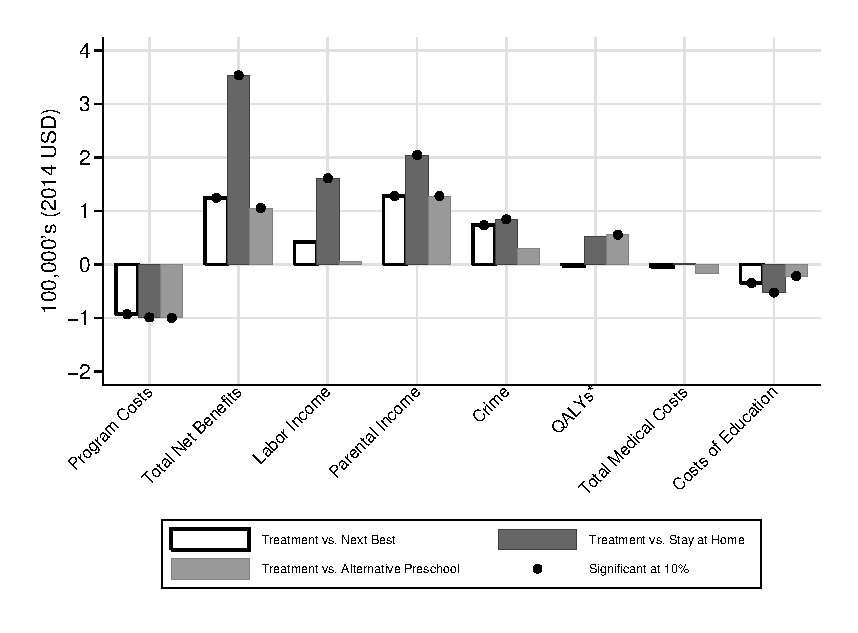
\includegraphics[width=.7\columnwidth]{output/abccare_npvs1.eps}
\floatfoot{
\footnotesize
Note: This figure displays the life-cycle net present values of the main components of the cost/benefit analysis of ABC/CARE from birth to age 79, discounted to birth at a rate of 3\%. ``Treatment vs. Control'': compares the treatment to the control group. ``Treatment vs. Stay at Home'': compares the treatment group to those subjects who stayed at home. ``Treatment vs. Alternative Preschool'': compares the treatment group to those subjects who attended alternative preschools. The latter two are based on matching estimators that account for selection on observable variables. By ``net" we mean that each component represents the total value for the treatment group minus the total value for the control group. Program costs: the total cost of implementing ABC/CARE. Total net benefits: the total net benefits of \textit{all} the components we consider. Labor income: total individual labor income from ages 20 to the retirement of program participants  (assumed to be age 67). Parental income: total parental labor income of the parents of the program participants from when the participants were ages 1.5 to 21. Crime: the total cost of crime (judicial and victimization costs). Total medical costs: both private and public medical costs from ages 15 to 79. Costs of education: the total costs of education of the individual from ages 6 to 26 and include any costs from special education and grade retention. For display simplicity, the following components are omitted from the figure: (i) cost of alternative preschool paid by the control group children parents; (ii) transfer income from the government; (iii) disability benefits and social security claims; and (iv) costs of increased maternal education. Inference is based on non-parametric, one-sided $p$-values from the empirical bootstrap distribution. We highlight point estimates significant at the $10\%$ level.\\
*QALYs refers to the quality-adjusted life years. Any gain corresponds to better health conditions through age 79.\\
}
\end{sidewaysfigure}

\begin{sidewaysfigure}[!htbp]
\caption{Life-cycle Net Present Value of Main Components of the CBA, Males}
\label{figure:npvsm}
\centering
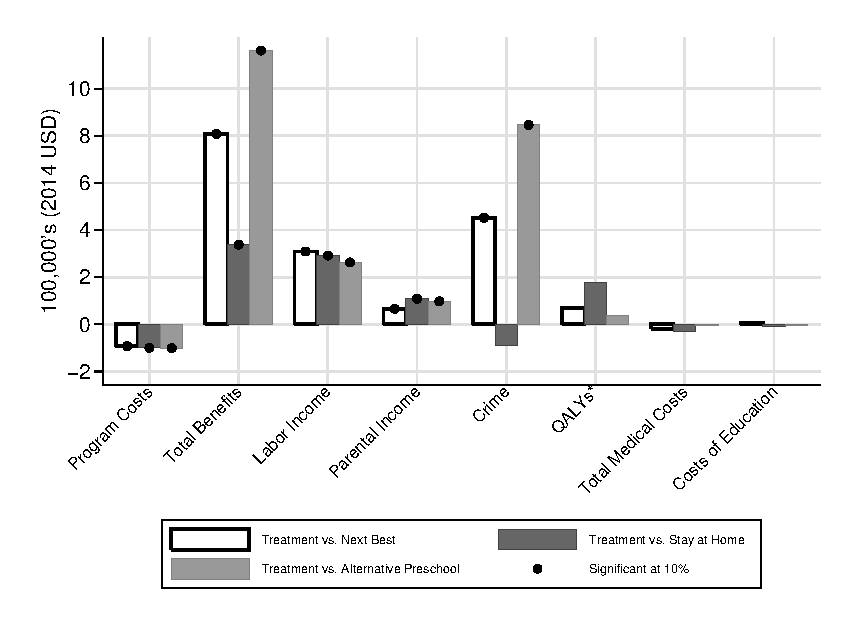
\includegraphics[width=.7\columnwidth]{output/abccare_npvs2.eps}
\floatfoot{
\footnotesize
Note: This figure displays the life-cycle net present values of the main components of the cost/benefit analysis of ABC/CARE from birth to age 79, discounted to birth at a rate of 3\%. ``Treatment vs. Control'': compares the treatment to the control group. ``Treatment vs. Stay at Home'': compares the treatment group to those subjects who stayed at home. ``Treatment vs. Alternative Preschool'': compares the treatment group to those subjects who attended alternative preschools. The latter two are based on matching estimators that account for selection on observable variables. By ``net" we mean that each component represents the total value for the treatment group minus the total value for the control group. Program costs: the total cost of implementing ABC/CARE. Total net benefits: the total net benefits of \textit{all} the components we consider. Labor income: total individual labor income from ages 20 to the retirement of program participants  (assumed to be age 67). Parental income: total parental labor income of the parents of the program participants from when the participants were ages 1.5 to 21. Crime: the total cost of crime (judicial and victimization costs). Total medical costs: both private and public medical costs from ages 15 to 79. Costs of education: the total costs of education of the individual from ages 6 to 26 and include any costs from special education and grade retention. For display simplicity, the following components are omitted from the figure: (i) cost of alternative preschool paid by the control group children parents; (ii) transfer income from the government; (iii) disability benefits and social security claims; and (iv) costs of increased maternal education. Inference is based on non-parametric, one-sided $p$-values from the empirical bootstrap distribution. We highlight point estimates significant at the $10\%$ level.\\
*The treatment vs. stay at home net present value is sizable and negative (-\$91,476.3); its standard error is 86,657.3.\\
**QALYs refers to the quality-adjusted life years. Any gain corresponds to better health conditions through age 79.\\
}
\end{sidewaysfigure}


\subsection{Using our Estimates to Understand Recent Benefit/Cost Analyses}

We use our analysis to examine the empirical foundations of the approach to benefit/cost analysis taken a prototypical study of \citet{Kline_Walters_2016_QJE}. They use data on the Head Start Impact Study (HSIS) and report a benefit/cost ratio between $1.50$ and $1.84$.\footnote{HSIS is a one-year-long randomized evaluation of Head Start.} Their analysis proceeds in three steps: (i) calculate the treatment effect on IQ around age 4.5\footnote{An index based on the Peabody Picture Vocabulary and Woodcock Johnson III Tests.} at age 5; (ii) monetize this gain using the return to the IQ measured between ages 5 and 7 in terms of net present value of labor income at age 27 \citep{Chetty_Friedman_etal_2011_QJoE}.\footnote{\citet{Chetty_Friedman_etal_2011_QJoE} return is based on Stanford Achievement Tests.}$^,$\footnote{For this comparison exercise, we interpret the earnings estimated in \citet{Chetty_Friedman_etal_2011_QJoE} to be equivalent to labor income.} Calculations from \citet{Chetty_Friedman_etal_2011_QJoE} indicate that a 1 standard deviation gain in IQ at age 5 implies a $13.1\%$ increase in the net present value of labor income through age 27;\footnote{This is based on combining information from Project Star and administrative data at age 27.} and (iii) calculate the benefit/cost ratio based on this gain and their own calculations of the program's cost.\footnote{Their calculation assigns the net present value of labor income through age 27 of $\$385,907.17$ to the control-group participants, as estimated by  \citet{Chetty_Friedman_etal_2011_QJoE}.}$^,$\footnote{All money values that we provide in this section are in 2014 USD. We discount the value provided by \citet{Chetty_Friedman_etal_2011_QJoE} to the age of birth of the children in our sample (first cohort).}


\begin{table}[!htbp]
\begin{threeparttable}
\caption{Alternative Cost-benefit Analyses Calculations}
\label{table:comparing}
\centering
\footnotesize

\begin{tabular}{cllcc}
\toprule
Age & \mc{1}{c}{NPV Source} & Component & \citet{Kline_Walters_2016_QJE} & Authors' Method \\
& & & Method & \\
\midrule
\multirow{2}{*}{27} & \cite{Chetty_Friedman_etal_2011_QJoE} & Labor income & 0.58 (s.e. 0.28) &  \\
& ABC/CARE-calculated & Labor income & 0.09 (s.e. 0.04) &  1.09 (s.e. 0.04)\\
\midrule
\multirow{2}{*}{34} & ABC/CARE-calculated & Labor income & 0.37 (s.e. 0.04) & 0.15 (s.e. 0.05) \\
& ABC/CARE-calculated & All & 1.21 (s.e. 0.05) &  3.20 (s.e. 1.04) \\
\midrule
\multirow{2}{*}{Life-cycle} &  ABC/CARE-calculated & Labor income & 1.56 (s.e. 0.08) & 1.55 (s.e. 0.76) \\
& ABC/CARE-calculated & All & 3.80 (s.e. 0.29) & 7.33 (s.e. 1.84) \\
\bottomrule
\end{tabular}

\begin{tablenotes}
\footnotesize
\item Note: This table displays benefit/cost ratios based on the methodology in \citet{Kline_Walters_2016_QJE} and based on our own methodology. Age: age at which we stop calculating the net-present value. NPV Source: source where we obtain the net present value. Component: item used to compute net present value (all refers to the net present value of all the components). \citet{Kline_Walters_2016_QJE} Method: estimate based on these authors methodology. Author's Method: estimates based on our methodology. Standard errors are based on the empirical bootstrap distribution.
\end{tablenotes}
\end{threeparttable}
\end{table}

To analyze how our estimates compare to those based on the method in \citet{Kline_Walters_2016_QJE}, we display a series of exercises in the fourth column of Table~\ref{table:comparing}. For purposes of comparison, the fifth column of Table~\ref{table:comparing} shows the analogous estimates based on our own method.

In the first exercise, we use both the ``return to IQ'' and the net-present value of labor income at age 27 reported in  \citet{Chetty_Friedman_etal_2011_QJoE}. In the second exercise, we perform a similar exercise but we use our own estimate of the net-present value of labor income at age 27.\footnote{This allows us to compute our own ``return to WPPSI'' and impute it to the treatment-group individuals.} The remaining exercises are similar, but (i) increase the age range over which we calculate the net-present value of labor income; or (ii) consider the value of all the lifetime components we analyze throughout the paper.

Our methodology: provides a more accurate estimate of the net-present value (and the return to IQ) of the components. We better quantify the effects of the analyzed experiment by considering the whole life-cycle; we also better approximate the statistical uncertainty of our estimates by considering both the sampling error in the experimental and non-experimental samples and the prediction error due to the interpolation and extrapolation. Proceeding in this fashion enables us to an extensive sensitivity analysis of each of the components we monetize.

\section{Summary} \label{section:conclusion}

This paper studies two influential early childhood interventions evaluated by the method of randomized control trials with long term follow up through age 34. These programs are being emulated in a variety of active interventions around the world. We document outcomes across multiple life domains. We find an aggregate benefit/cost ratio of 5.6 and a rate of return of 13\% per annum, even after adjusting for welfare costs of financing the program through public revenue.

To reach these conclusions, we face and address a number of empirical challenges: (a) control group substitution; (b) extrapolating lifetime benefits beyond the experimental period; and (c) multiple hypothesis testing. Our approach serves as a template for economic evaluations of programs with partial follow up over the life cycle.

We find that benefits differ substantially by gender. Females have more beneficial treatment effects than males, but the monetized value of the male treatment effects are greater. There are substantial effects on health and the quality of life and on crime for males. For females, the benefits are concentrated on education, employment, and minor crimes. The effects for females are stronger compared to staying at home. The effects for males are stronger compared to participation in alternative preschools. The program subsidizes causal effect on maternal labor income. We establish the benefits of analyzing long term multiple benefits of this intervention.

%References
\singlespace
\bibliographystyle{chicago}
\bibliography{heckman}

\end{document} 